
% AGUJournalTemplate.tex: this template file is for articles formatted with LaTeX
%
% This file includes commands and instructions
% given in the order necessary to produce a final output that will
% satisfy AGU requirements, including customized APA reference formatting.
%
% You may copy this file and give it your
% article name, and enter your text.
%
%
% Step 1: Set the \documentclass
%
%

%% To submit your paper:
\documentclass[draft]{agujournal2019}
\usepackage{url} %this package should fix any errors with URLs in refs.
\usepackage{lineno}
\usepackage[inline]{trackchanges} %for better track changes. finalnew option will compile document with changes incorporated.
\usepackage{soul}
\linenumbers

%%%%%%%
% As of 2018 we recommend use of the TrackChanges package to mark revisions.
% The trackchanges package adds five new LaTeX commands:
%
%  \note[editor]{The note}
%  \annote[editor]{Text to annotate}{The note}
%  \add[editor]{Text to add}
%  \remove[editor]{Text to remove}
%  \change[editor]{Text to remove}{Text to add}
%
% complete documentation is here: http://trackchanges.sourceforge.net/
%%%%%%%

\draftfalse

%% Enter journal name below.
%% Choose from this list of Journals:
%
% JGR: Atmospheres
% JGR: Biogeosciences
% JGR: Earth Surface
% JGR: Oceans
% JGR: Planets
% JGR: Solid Earth
% JGR: Space Physics
% Global Biogeochemical Cycles
% Geophysical Research Letters
% Paleoceanography and Paleoclimatology
% Radio Science
% Reviews of Geophysics
% Tectonics
% Space Weather
% Water Resources Research
% Geochemistry, Geophysics, Geosystems
% Journal of Advances in Modeling Earth Systems (JAMES)
% Earth's Future
% Earth and Space Science
% Geohealth
%
% ie, \journalname{Water Resources Research}

\journalname{Journal of Advances in Modeling Earth Systems (JAMES)}


\begin{document}

%% ------------------------------------------------------------------------ %%
%  Title
%
% (A title should be specific, informative, and brief. Use
% abbreviations only if they are defined in the abstract. Titles that
% start with general keywords then specific terms are optimized in
% searches)
%
%% ------------------------------------------------------------------------ %%

% Example: \title{This is a test title}

\title{Impact of grids and dynamical cores in CESM2.2 on the surface mass balance of the Greenland Ice Sheet}

%% ------------------------------------------------------------------------ %%
%
%  AUTHORS AND AFFILIATIONS
%
%% ------------------------------------------------------------------------ %%

% Authors are individuals who have significantly contributed to the
% research and preparation of the article. Group authors are allowed, if
% each author in the group is separately identified in an appendix.)

% List authors by first name or initial followed by last name and
% separated by commas. Use \affil{} to number affiliations, and
% \thanks{} for author notes.
% Additional author notes should be indicated with \thanks{} (for
% example, for current addresses).

% Example: \authors{A. B. Author\affil{1}\thanks{Current address, Antartica}, B. C. Author\affil{2,3}, and D. E.
% Author\affil{3,4}\thanks{Also funded by Monsanto.}}
\authors{Adam R. Herrington\affil{1}, Peter H. Lauritzen\affil{1}, William H. Lipscomb\affil{1}, Marcus Lofverstrom\affil{2} $\ $and Andrew Gettelman\affil{1}}

 \affiliation{1}{National Center for Atmospheric Research, 1850 Table Mesa Drive, Boulder, Colorado, USA}
\affiliation{2}{Department of Geosciences, University of Arizona, 1040 E. 4th Street, Tucson, AZ USA}

% \affiliation{1}{First Affiliation}
% \affiliation{2}{Second Affiliation}
% \affiliation{3}{Third Affiliation}
% \affiliation{4}{Fourth Affiliation}

%\affiliation{=number=}{=Affiliation Address=}
%(repeat as many times as is necessary)

%% Corresponding Author:
% Corresponding author mailing address and e-mail address:

% (include name and email addresses of the corresponding author.  More
% than one corresponding author is allowed in this LaTeX file and for
% publication; but only one corresponding author is allowed in our
% editorial system.)

% Example: \correspondingauthor{First and Last Name}{email@address.edu}

\correspondingauthor{=name=}{=email address=}

%% Keypoints, final entry on title page.

%  List up to three key points (at least one is required)
%  Key Points summarize the main points and conclusions of the article
%  Each must be 140 characters or fewer with no special characters or punctuation and must be complete sentences

% Example:
% \begin{keypoints}
% \item	List up to three key points (at least one is required)
% \item	Key Points summarize the main points and conclusions of the article
% \item	Each must be 140 characters or fewer with no special characters or punctuation and must be complete sentences
% \end{keypoints}

\begin{keypoints}
\item enter point 1 here
\item enter point 2 here
\item enter point 3 here
\end{keypoints}

%% ------------------------------------------------------------------------ %%
%
%  ABSTRACT and PLAIN LANGUAGE SUMMARY
%
% A good Abstract will begin with a short description of the problem
% being addressed, briefly describe the new data or analyses, then
% briefly states the main conclusion(s) and how they are supported and
% uncertainties.

% The Plain Language Summary should be written for a broad audience,
% including journalists and the science-interested public, that will not have 
% a background in your field.
%
% A Plain Language Summary is required in GRL, JGR: Planets, JGR: Biogeosciences,
% JGR: Oceans, G-Cubed, Reviews of Geophysics, and JAMES.
% see http://sharingscience.agu.org/creating-plain-language-summary/)
%
%% ------------------------------------------------------------------------ %%

%% \begin{abstract} starts the second page

\begin{abstract}
[ enter your Abstract here ]
\end{abstract}

\section*{Plain Language Summary}
[ enter your Plain Language Summary here or delete this section]


%% ------------------------------------------------------------------------ %%
%
%  TEXT
%
%% ------------------------------------------------------------------------ %%

%%% Suggested section heads:
\section{Introduction}

General Circulation Models (GCMs) are powerful tools for understanding the meteorology and climate of the high-latitudes, which are among the most sensitive regions on Earth to global and environmental change. Despite their importance, the numerical treatment of polar regions in GCMs is handled in vastly-different ways due to the so-called \textit{pole-problem} \cite{W2007JMSJ}. The pole problem refers to numerical instability arising from the convergence of meridian lines into polar singularities on latitude-longitude grids (e.g., Figure~\ref{fig:uni-grids}a). Depending on the numerics, methods exist to suppress this instability, and latitude-longitude grids may be advantageous for polar processes as structures can be represented with more degrees of freedom than elsewhere in the computational domain. With the recent trend towards globally uniform unstructured grids, any potential benefits of latitude-longitude grids on polar regions may become a relic of the past. In this study a number of grids and dynamical cores (hereafter referred to as \textit{dycores}) available in the Community Earth System Model, version 2.2 (CESM; \url{http://www.cesm.ucar.edu/models/cesm2/}), including brand new variable-resolution grids, are evaluated to understand their impacts on the simulated characteristics of the Arctic, with a special focus on the climate and surface mass balance of the Greenland Ice Sheet.

In the 1970's the pole problem was largely defeated through wide-spread adoption of efficient spectral transform methods in GCMs. These methods transform grid point fields into a global, isotropic representation in wave space, where linear operators (e.g. horizontal derivatives) in the equation set can be solved for exactly. While spectral transform methods are still used in the 21st century, local numerical methods have become desirable for their ability to run efficiently on massively parallel systems. The pole problem has thus re-emerged in contemporary climate models that use latitude-longitude grids, and some combination of reduced grids and polar filters are necessary to ameliorate this instability \cite{JW2010LNCSE}. Polar filters are akin to a band-aid; they subdue the growth of unstable modes by applying additional damping to the solution over polar regions. This additional damping reduces the effective resolution in polar regions, and the resolved scales are approximately the same everywhere on the grid.

An alternative approach is to use unstructured grids, which allow for more flexible grid structures that permit quasi-uniform grid spacing globally and eliminates the pole-problem entirely (e.g., Figure~\ref{fig:uni-grids}c). This grid flexibility also permits variable-resolution or regional grid refinement (e.g., Figure~\ref{fig:vr-grids}). Grids can be developed with refinement over polar regions that could in principle make up for any loss in polar resolution in transitioning away from latitude-longitude grids (e.g., Figure~\ref{fig:vr-grids}), although this comes at the cost of a smaller CFL-limiting time-step in the refined region (the CFL-condition --- short for Courant–Friedrichs–Lewy condition --- is a necessary condition for numerical stability when using discrete data in time and space). Unstructured grids also scale more efficiently on parallel systems than latitude-longitude grids, likely resulting in a greater prevalence of unstructured grids as computing power continued to increase over time.

The meteorology and climate of the Arctic is characterized by a range of processes and scales that are difficult to represent in GCMs \cite{BETAL2001MWR,SG2017MWR,VETAL2018TC}. For example, while synoptic scale storms are generally well represented at typical GCM resolutions of 1 to 2 degrees \cite{JW2006QJR,IPCCAR5}, mesoscale Polar Lows are not well resolved at these resolutions. These mesoscale systems are prevalent during the cold season and produce gale-force winds that can induce large heat and moisture fluxes through the underlying sea-ice/ocean interface. The Arctic also contains the Greenland Ice Sheet (hereafter denoted as \textit{GrIS}). While it blankets the largest island in the world (Greenland), many of the processes that control the GrIS annual surface mass balance (the integrated sum of precipitation and runoff) are only partially resolved at typical GCM resolutions. For example, GrIS precipitation is typically confined to the ice-sheet margins (predominately the southeastern margin) where orographic precipitation is generated by steep topographic slopes. GrIS ablation areas (marginal regions where seasonal melting exceeds the annual mass input from precipitation) are typically 10s to 100\,km wide and confined to low-level areas or regions with limited precipitation. GCMs struggle to resolve the magnitude and extent of these features \cite{VETAL2018TC}, which can lead to unrealistic ice sheet growth in models with an interactive ice sheet component \cite<e.g.,>{LETAL2020JAMES}. 

The goal of this study is to characterize the representation of high-latitude regions using the spectral-element and finite-volume dycores in CESM2.2, as these models treat the high-latitudes, e.g., the pole-problem, in different ways. The manuscript is laid out as follows: Section~\ref{sec:methods} consists of documentation of the grids, dycores and physical parameterizations used in this study. The Arctic refined grids were developed by the authors, and this section serves as their official documentation in CESM2.2. Section~\ref{sec:methods} also contains a description of the experiments along with reanalysis datasets and post-processing software used for evaluating the model simulations. Section~\ref{sec:results} contains the results of the experiments, followed by Section~\ref{sec:conclusions} that provides a general discussion and conclusions.

\begin{figure}[t]
\begin{center}
\begin{tabular}{cc}
         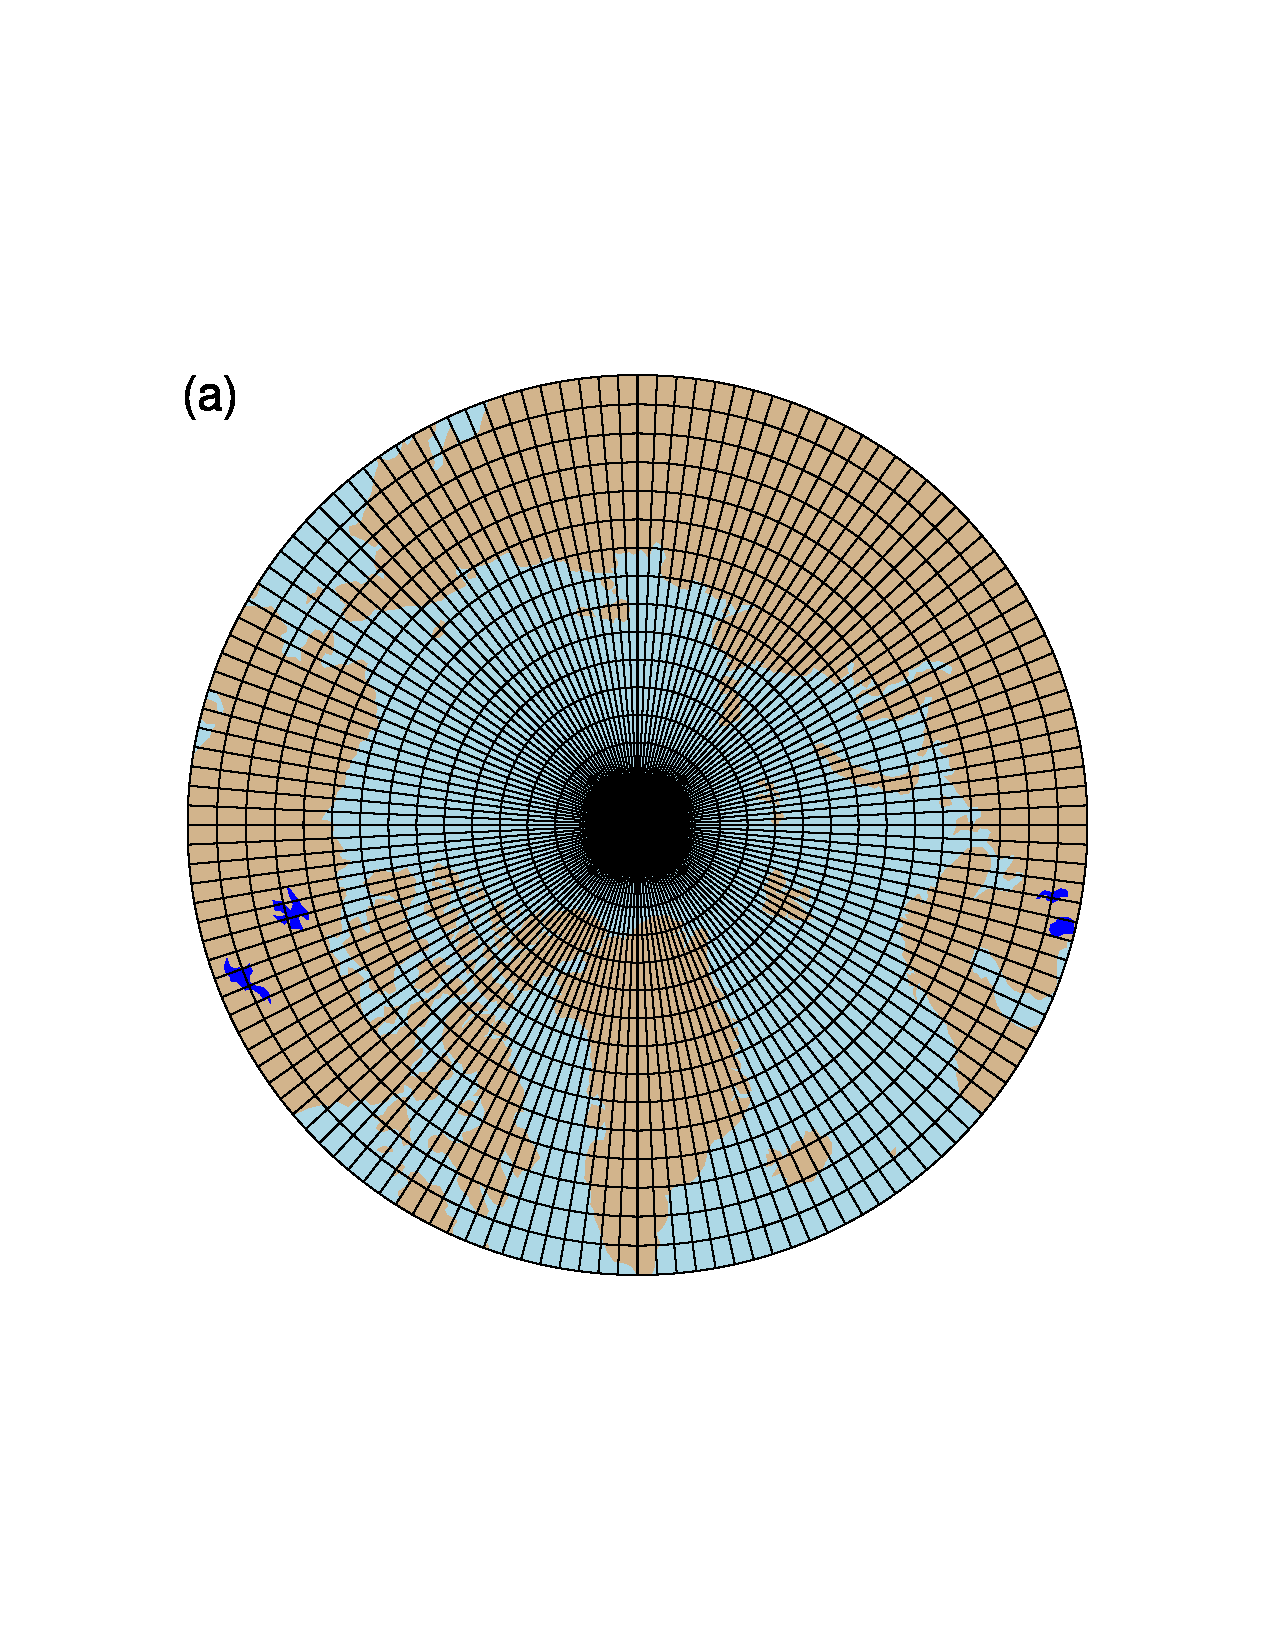
\includegraphics[width=60mm]{figs/grid-f19.pdf}&
         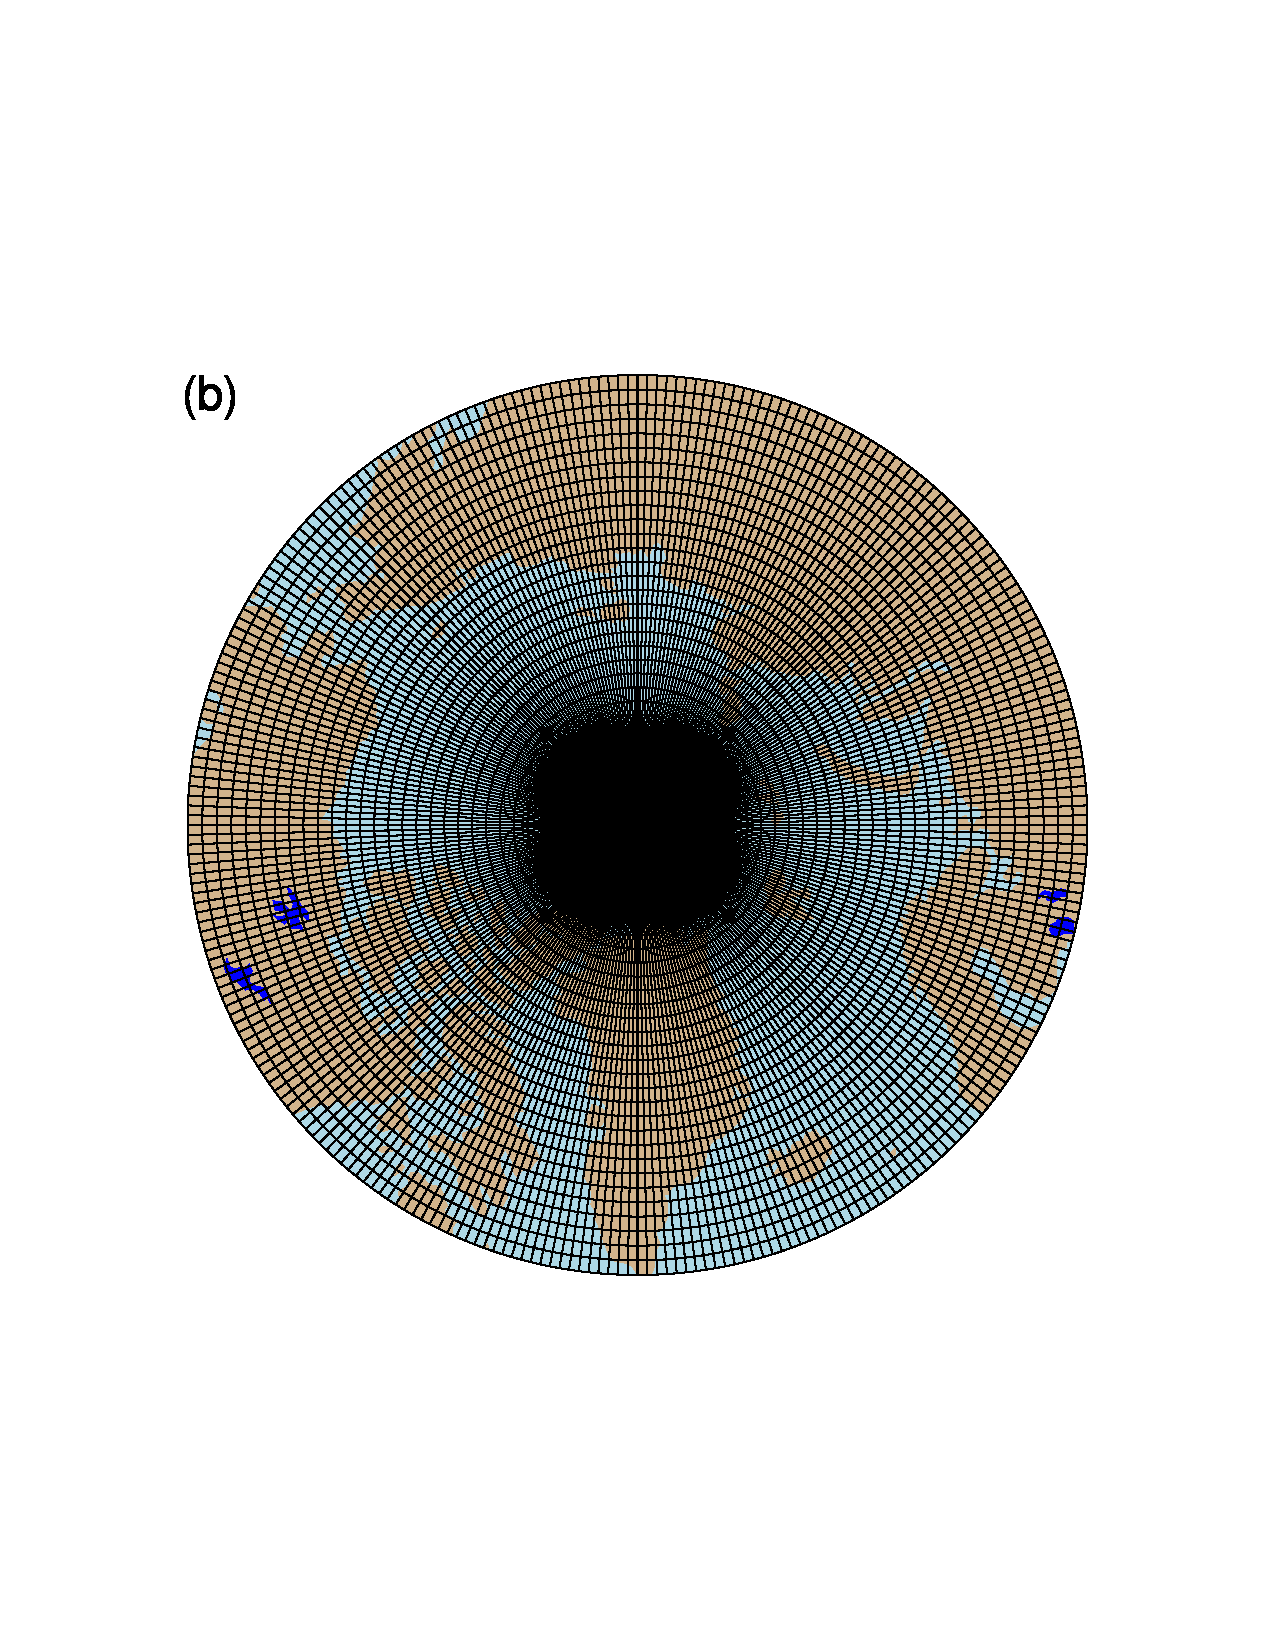
\includegraphics[width=60mm]{figs/grid-f09.pdf}\\
         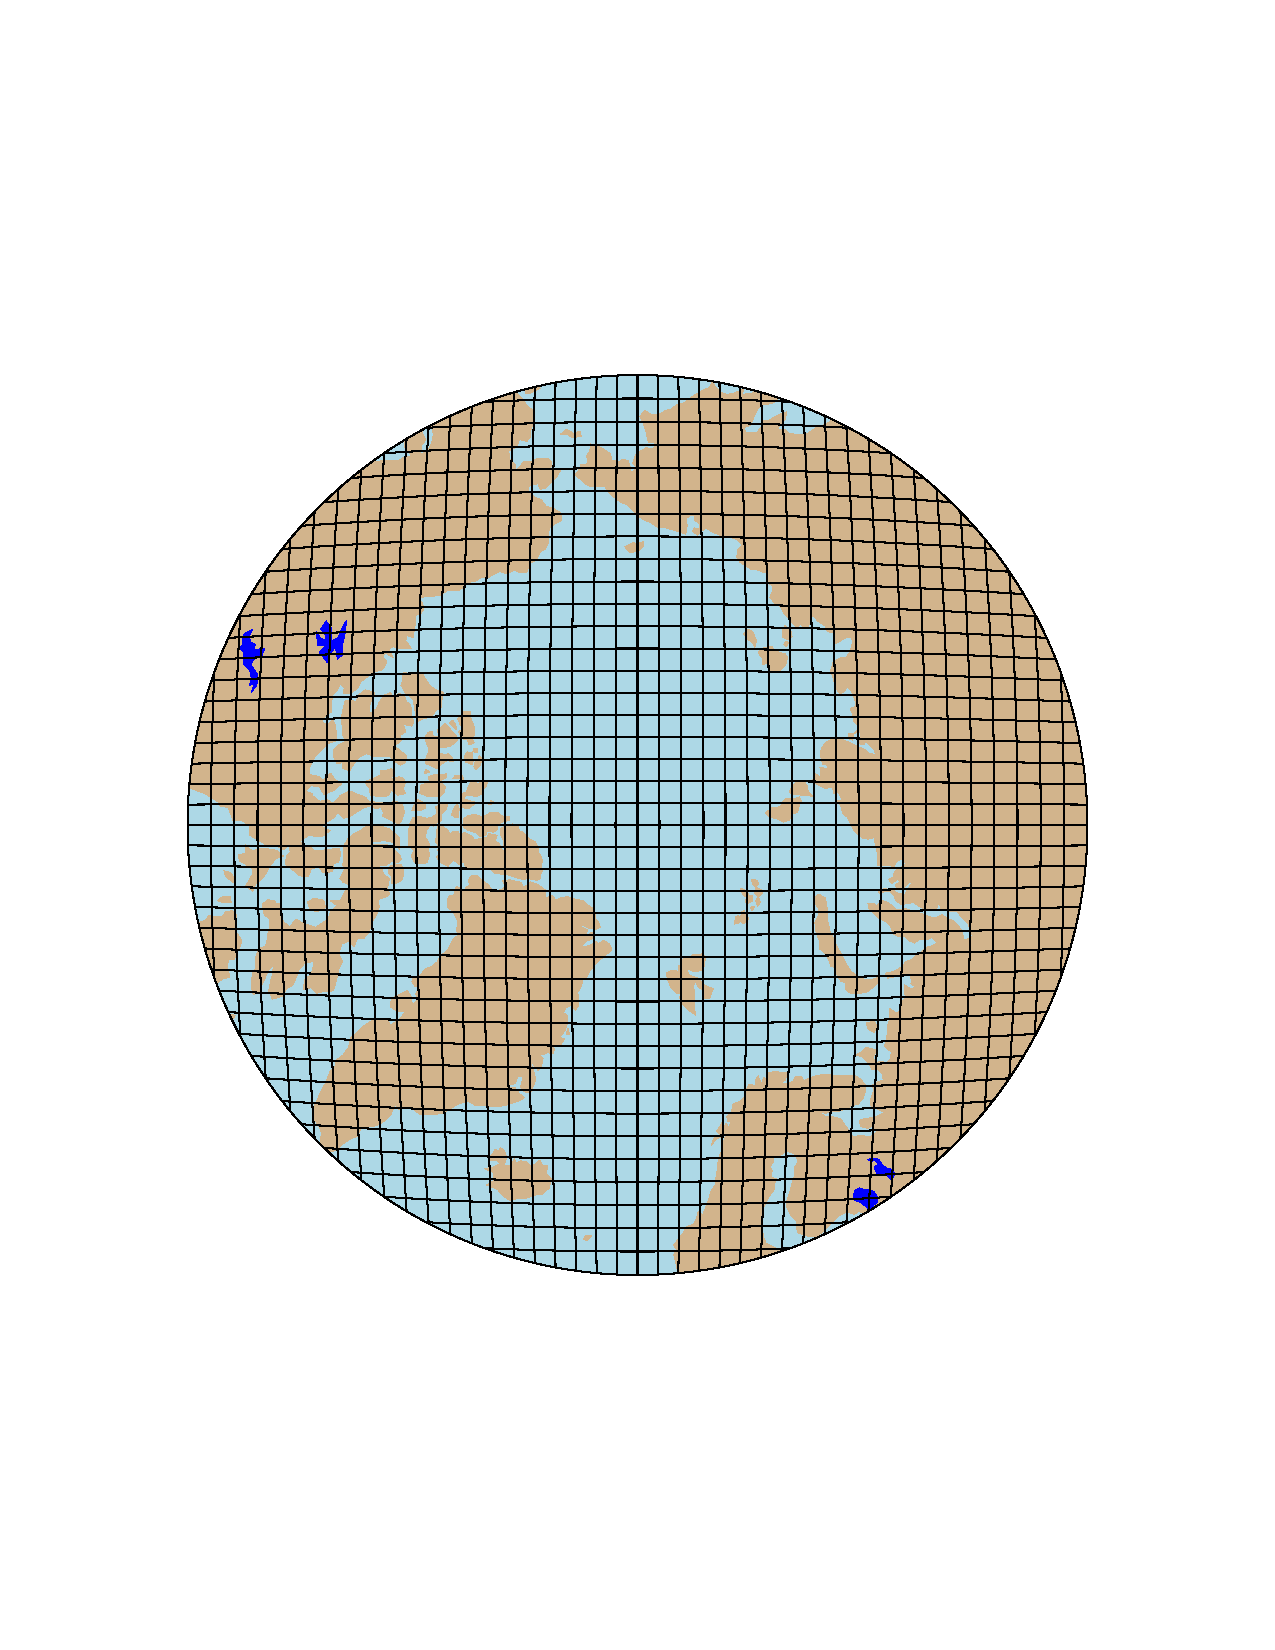
\includegraphics[width=60mm]{figs/grid-ne30pg2.pdf}&
         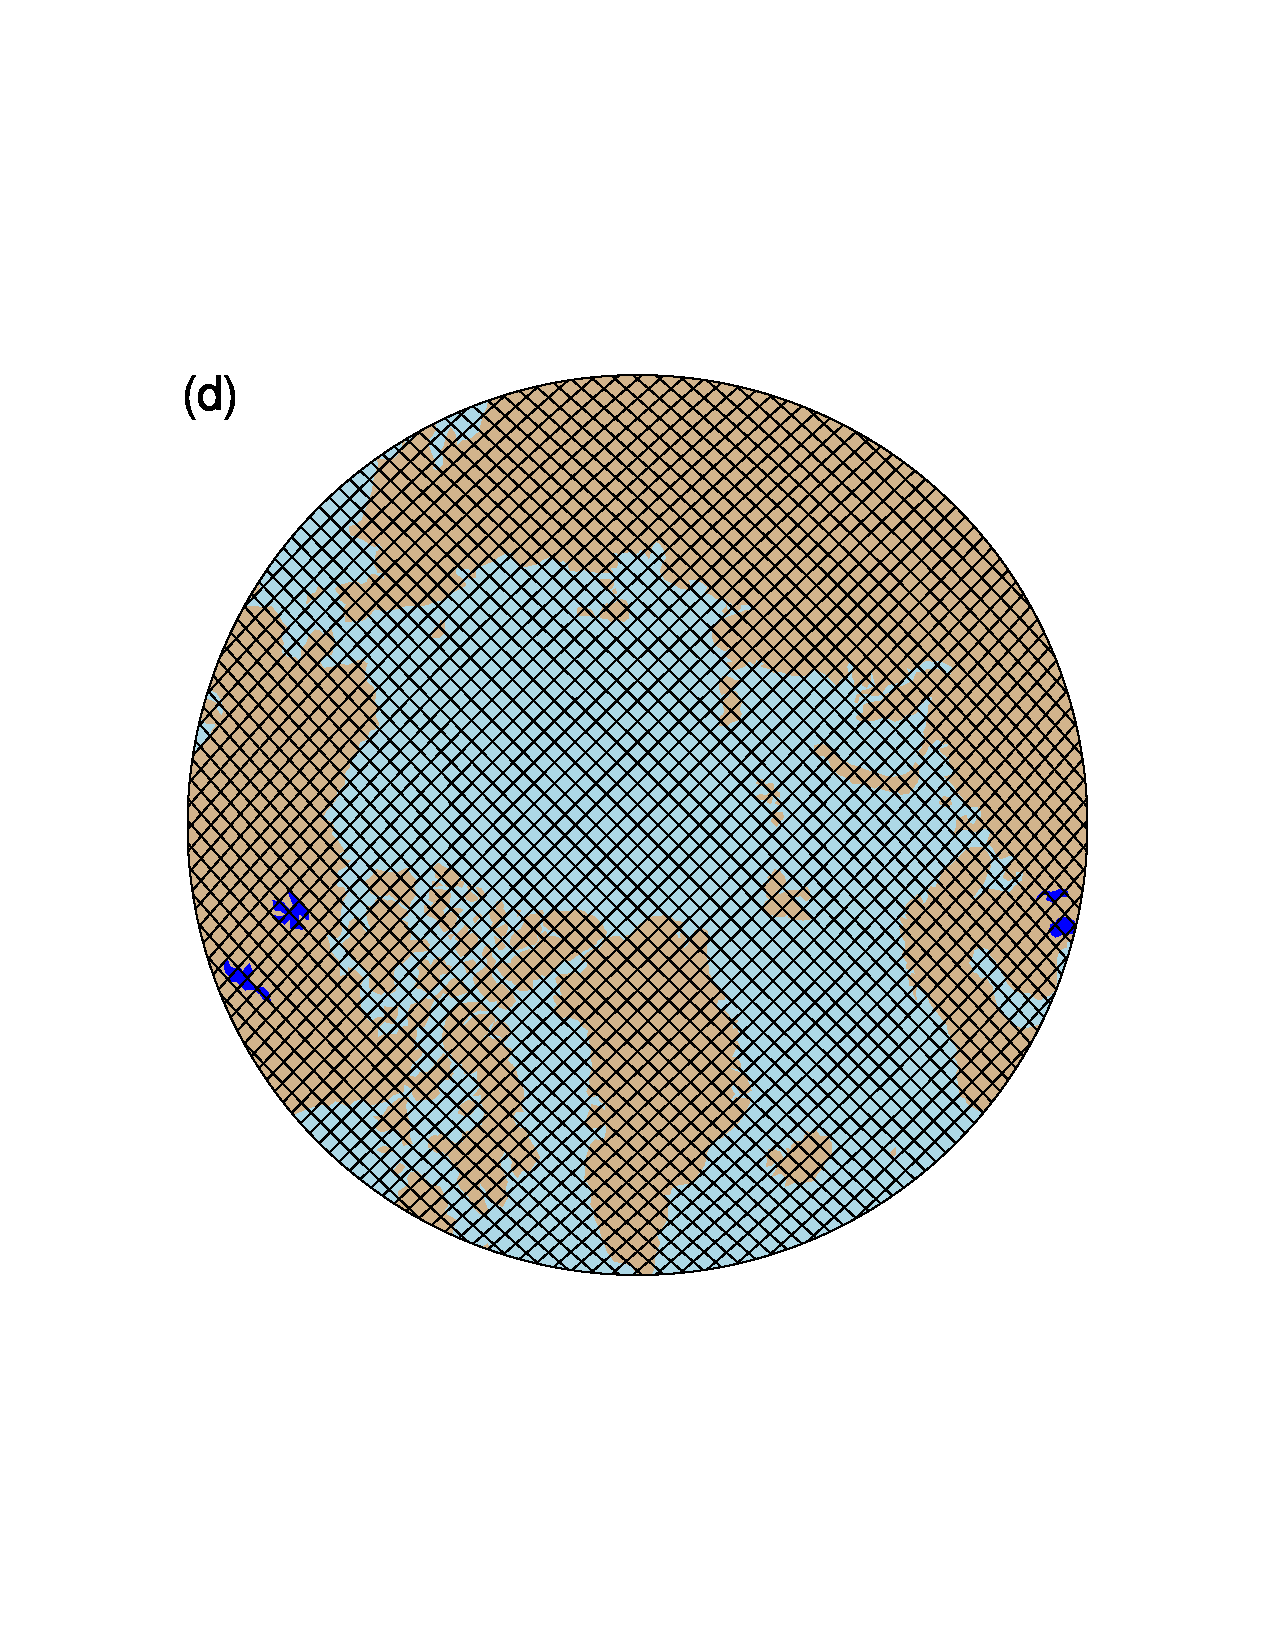
\includegraphics[width=60mm]{figs/grid-ne30pg3.pdf} \\
\end{tabular}
\end{center}
\caption{Computational grids for the uniform $1^{\circ}-2^{\circ}$ grids in this study.}
\label{fig:uni-grids}
\end{figure}

\begin{figure}[t]
\begin{center}
\begin{tabular}{cccc}
         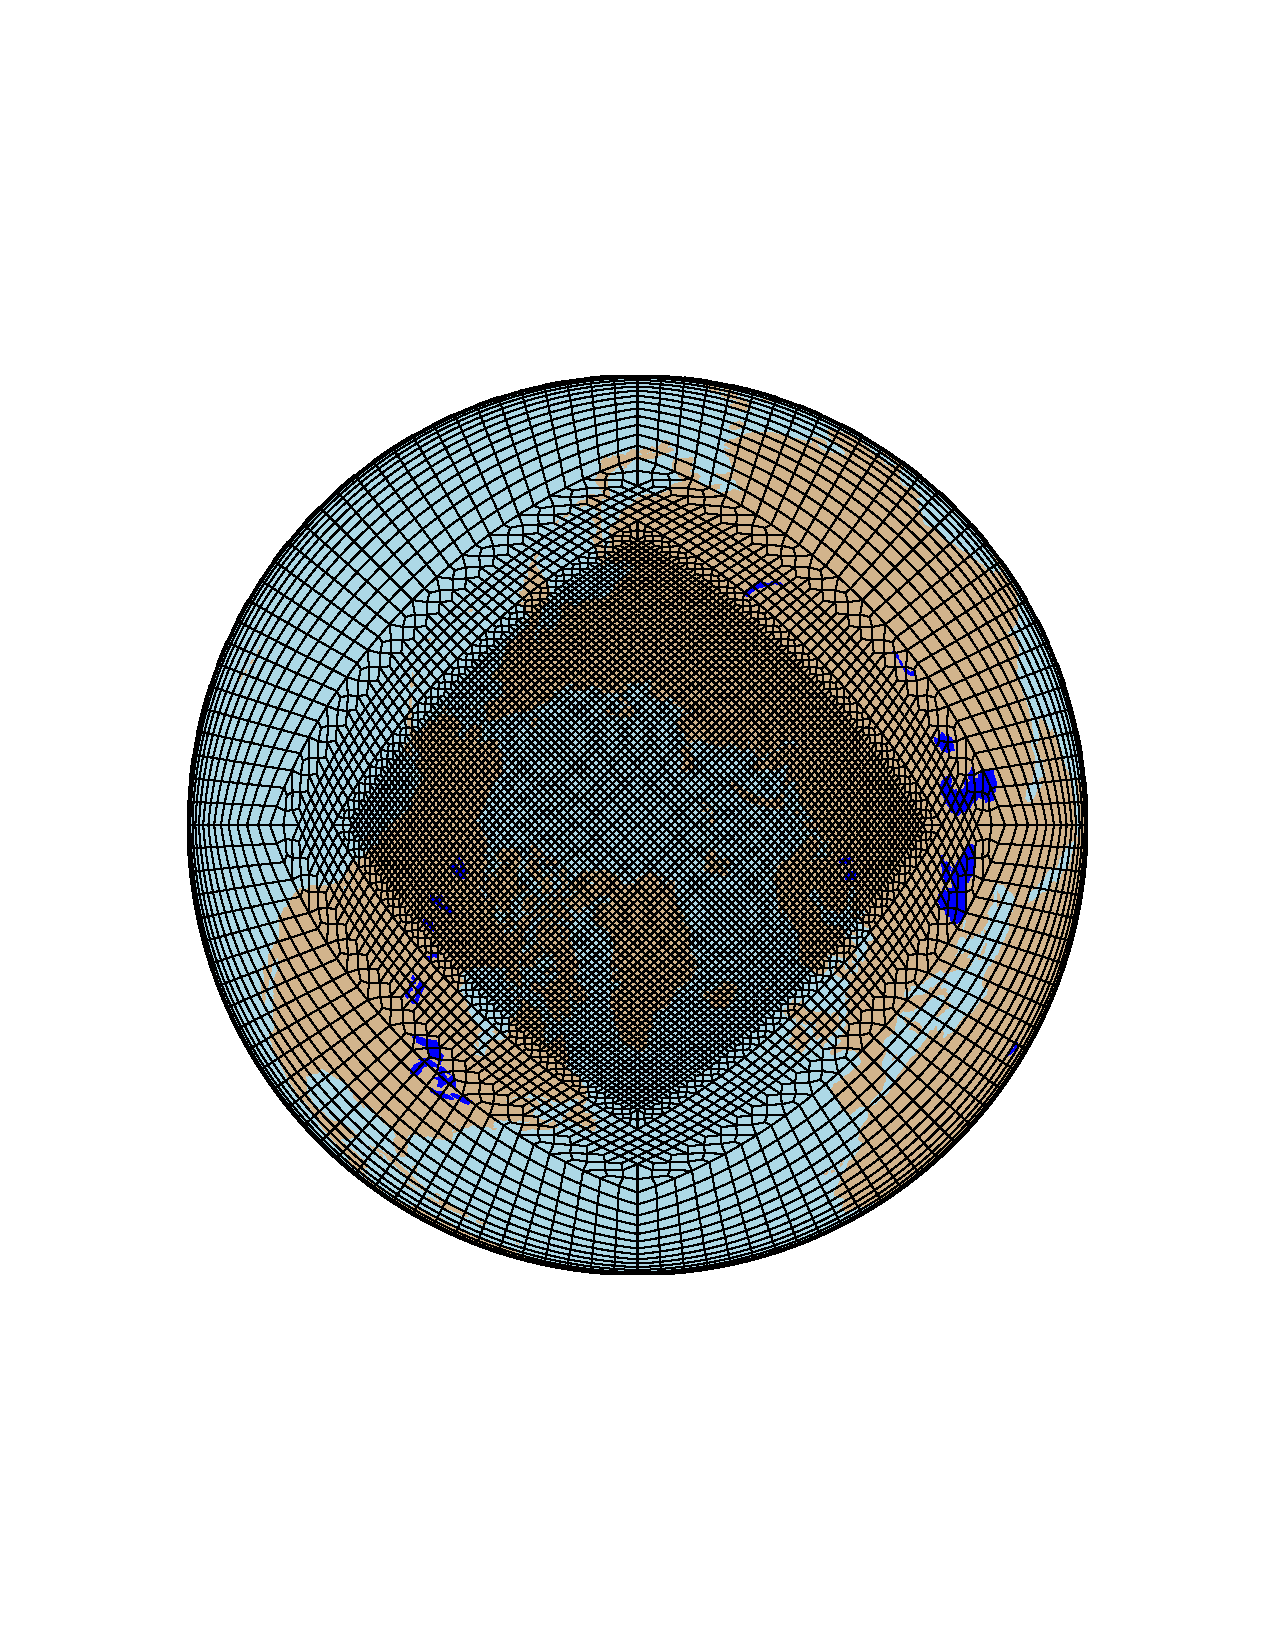
\includegraphics[width=60mm]{figs/grid-ARCTIC.pdf}&
         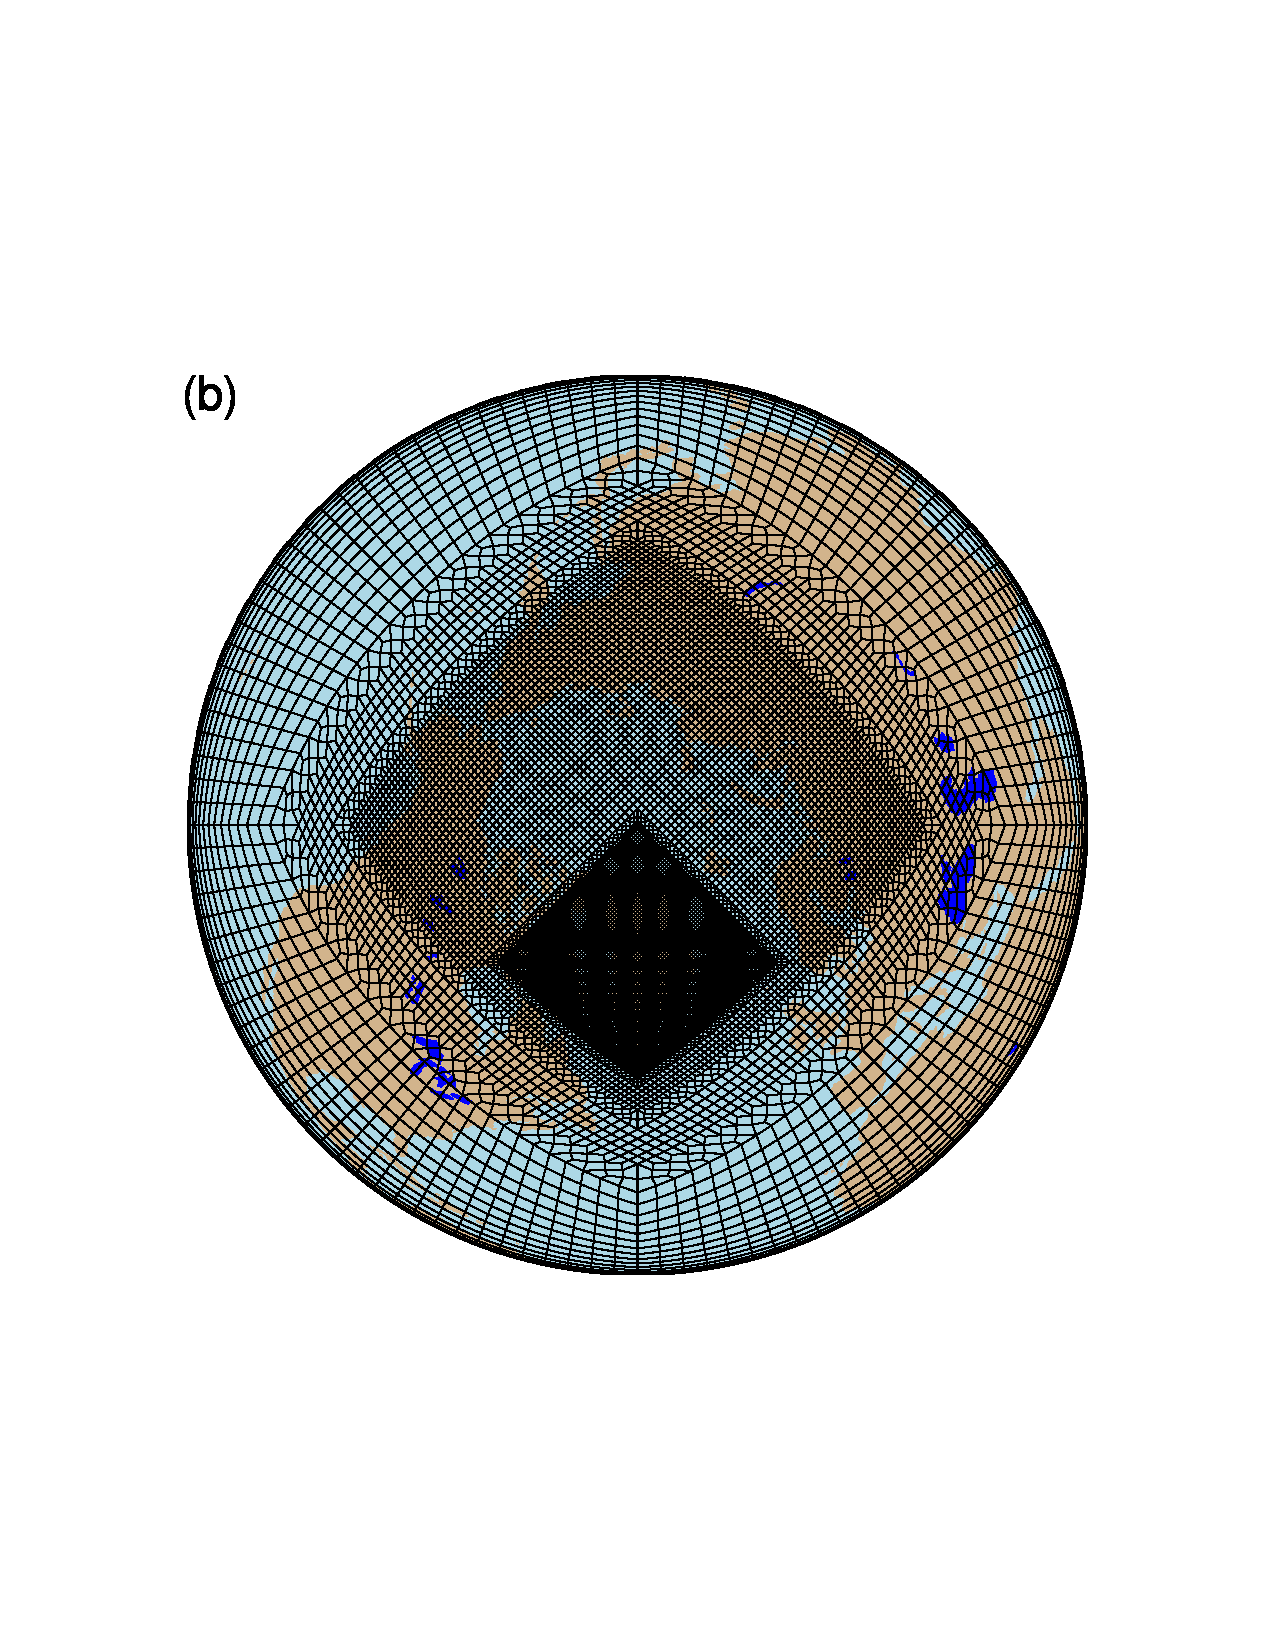
\includegraphics[width=60mm]{figs/grid-ARCTICGRIS.pdf} \\
\end{tabular}
\end{center}
\caption{Spectral-element grid for the variable-resolution ARCTIC grid in this study. Note that this is not the computational grid; each element has $3\times3$ independent grid points.}
\label{fig:vr-grids}
\end{figure}

\section{Methods}\label{sec:methods}
\subsection{Dynamical cores}

The atmospheric component of CESM2.2, the Community Atmosphere Model, version 6.3 \cite<CAM;>{CAM63}, supports a number of different atmospheric dynamical cores. These include dycores using latitude-longitude grids, such as finite-volume \cite<FV;>{L2004MWR} and eulerian spectral transform \cite<EUL;>{CETAL006JC} models, and dycores built on unstructured grids, including spectral-element \cite<SE;>{LetAl2018JAMES} and finite-volume 3 \cite<FV3;>{PL2007JCP} models. The EUL dycore is the oldest dycore in CAM, and the least supported of all the dycores. FV3 is the newest dycore in CAM, but it was not fully incorporated at the time this work commenced; both the EUL and FV3 dycores are omitted from this study. As such, the results presented in this study are comparing the performance of the SE and FV dycores.

\subsubsection{Finite-volume (FV) dynamical core}

The FV dycore is a hydrostatic model that integrates the equations of motion using a finite-volume discretization on a spherical latitude-longitude grid \cite{LR1997QJR}. The 2D dynamics evolve in floating Lagrangian layers that are periodically mapped to Eulerian reference grid in the vertical \cite{L2004MWR}, using a hybrid-pressure vertical coordinate. Hyperviscous damping is applied to the divergent modes while Laplacian damping is applied to momentum in the top few layers, referred to as a \textit{sponge layer} \cite{L2011IJHPC}. A polar filter is used to avoid computational instability due to the convergence of the meridians, allowing for a more practical time-step. It takes the form of a Fourier filter in the zonal direction, with the damping coefficients increasing monotonically in the poleward direction \cite{ST1995GEOS}.

\subsubsection{Spectral-element (SE) dynamical core}

The SE dycore is a hydrostatic model that integrates the equations of motion using a high-order continuous Galerkin method \cite{TTI1997JCP,TF2010JCP}. The computational domain is a cubed-sphere grid tiled with quadrilateral elements (e.g., Figure~\ref{fig:vr-grids}). Each element contains a fourth order basis set in each horizontal direction, with the solution defined at the roots of the basis functions, the Gauss-Lobatto-Legendre (GLL) quadrature points. This results in 16 GLL nodal points within each element, with 12 of the points lying on the (shared) element boundary. Communication between elements happens via the direct stiffness summation \cite{canuto2007}, which applies a numerical flux to the element boundaries that reconciles overlapping nodal values and produces a continuous global basis set. 

As with the FV dycore, the dynamics evolve in floating Lagrangian layers that are subsequently mapped to an Eulerian reference grid. A dry mass vertical coordinate was more recently implemented for thermodynamic consistency with condensates \cite{LetAl2018JAMES}. The 2D dynamics have no implicit dissipation and so hyperviscosity operators are applied to all prognostic variables to remove spurious numerical errors \cite{DetAl2012IJHPCA}. Laplacian damping is applied in the sponge layer.

The SE dycore supports regional grid refinement via its variable-resolution configuration, requiring two enhancements over uniform resolution grids. (1) As the numerical viscosity increases with resolution, explicit hyperviscosity relaxes according to the local element size, reducing in strength  by an order of magnitude per halving of the grid spacing. A tensor-hyperviscosity formulation is used \cite{GetAl2014GMD}, which adjusts the coefficients in two orthogonal directions to more accurately target highly distorted quadrilateral elements. (2) The topography boundary conditions need to be smoothed in a way that does not excite grid scale modes, and so the NCAR topography software \cite{gmdd-8-4623-2015} has been modified to scale the smoothing radius by the local element size. 

For spectral-element grids with quasi-uniform grid spacing, a variant in which tracer advection is computed using the Conservative Semi-Lagrangian Multi-tracer transport scheme (CSLAM) is used instead \cite<>{LTOUNGK2017MWR}. CSLAM has improved tracer property preservation and accelerated multi-tracer transport. It uses a separate grid from the spectral-element dynamics, through dividing each element into $3\times3$ control volumes with quasi-equal area. The physical parameterizations are computed from the state on the CSLAM grid, which has clear advantages over the default SE dycore in which the physics are evaluated at the GLL nodal points \cite{HL2018MWR}. 

\subsection{Grids}

Six grid are evaluated in this study (Table~\ref{tbl:table1}). The FV dycore is run with $1^{\circ}$ and $2^{\circ}$ grid spacing, referred to as $f09$ and $f19$, respectively (Figure~\ref{fig:uni-grids}a,b). The $1^{\circ}$ equivalent of the CAM-SE-CSLAM grid is also run, referred to as $ne30pg3$ (Figure~\ref{fig:uni-grids}c), where $ne$ refers to a grid with of $ne \times ne$ elements per cubed-sphere face, and $pg$ denotes that there are $pg \times pg$  control volumes per element for computing the physics. An additional $1^{\circ}$ CAM-SE-CSLAM grid is run, but with the physical paramerizations computed on a grid that contains $2\times2$ control volumes per element, $ne30pg2$ \cite<Figure~\ref{fig:uni-grids}d;>{HETAL2019JAMES}.

Two variable resolution meshes were developed as part of the CESM2.2 release that contains grid refinement over the Arctic (Figure~\ref{fig:vr-grids}). The Arctic meshes were developed using the software package SQuadgen (\url{https://github.com/ClimateGlobalChange/squadgen}). The $ARCTIC$ grid is a $1^{\circ}$ grid with $\frac{1}{4}^{\circ}$ regional refinement over the broader Arctic region. The $ARCTICGRIS$ grid is identical to the $ARCTIC$ grid, but contains an additional patch covering the big island of Greenland with $\frac{1}{8}^{\circ}$ resolution.

 \begin{table*}
 \centering
 \scriptsize
 \begin{tabular}{lccccc}
   \hline
   grid name & dycore & $\Delta x_{eq}$ (km) & $\Delta x_{refine}$ (km) & $\Delta t_{phys}$ (s) \\ 
   \hline
   $f19$ & FV & 278 & - &1800 \\
   $f09$ & FV & 139 & - &1800 \\
   $ne30pg2$ & SE-CSLAM & 167 & - & 1800 \\
   $ne30pg3$ & SE-CSLAM & 111 & - & 1800 \\
   $ARCTIC$ & SE & 111 & 28 & 450 \\
   $ARCTCIGRIS$ & SE & 111 & 14 & 225 \\
 \hline
 \end{tabular}
  \caption{Grids and dycores used in this study. $\Delta x_{eq}$ refers to average equatorial grid spacing, $\Delta x_{refine}$ refers to grid spacing in the refined region (if applicable) and $\Delta t_{phys}$ refers to the physics time-step. The dycore abbreviation FV refers to the finite-volume dycore, SE the spectral-element dycore and SE-CSLAM the spectral-element dycore w/ CSLAM tracer advection.}
 \label{tbl:table1}
 \end{table*}

\subsection{Physical parameterizations}

The CAM6 physical parameterization package (hereafter referred to as the \textit{physics}; \url{https://ncar.github.io/CAM/doc/build/html/index.html}) is used in all simulations in this study. CAM6 physics is most noteably different from it's predecessors through the incorporation of high-order turbulence closure, Cloud Layers Unified by Binormals \cite<CLUBB;>{GETAL2002JAS,BOG2013JCLIM}, which jointly acts as a PBL, shallow convection and cloud macrophysics scheme. CLUBB is coupled with the MG2 microphysics scheme \cite{MG2}, with prognostic precipitation and classical nucleation theory in representing cloud ice for improved cloud-aerosol interactions. Deep convection is parameterized using a convective quasi-equilibrium mass flux scheme \cite{ZM1995AO,NRJ2008JC} inlcuding convective momentum transport \cite{RSG2010JAS}. PBL form drag is modeled after \cite{BBW2004QJRMS} and orographic gravity wave drag is represented with an anisotropic method informed by the orientation of topographic ridges at the sub-grid scale. 

All grids and dycores in this study use 32 levels in the vertical, with a model top of about $1 \ hPa$ or about $40 \ km$. The physics time-step is dependent on grid resolution. Increases in horizontal resolution permit faster vertical velocities that reduce characteristic time-scales, and so the physics time-step is reduced to avoid large time truncation errors \cite{HR2018JAMES}. The $ARCTIC$ and $ARCTICGRIS$ grids are therefore run with a $4\times$ and $8\times$ reduction in physics time-step relative to the default 1800 s time-step used in coarser, uniform resolution grids (Table~\ref{tbl:table1}.

Initial simulations with the $ne30pg3$ spectral-element grid produced weaker shortwave cloud forcing relative to the tuned up finite-volume dycore. All runs with the spectral-element dycore have two CLUBB parameter changes in order to provide a more realistic cloud forcing and top-of-atmosphere radiation balance. These are CLUBB's $gamma$ parameter, reduced from 0.308 to 0.270, and c14, reduced from 2.2 to 1.6. Briefly, the $gamma$ parameter scales the width of the sub-grid distribution of vertical velocity, and c14 controls the strength of the damping term in the equation for the horizontal component of turbulent kinetic energy. For a thorough explanation of how CLUBB parameters impact the simulated climate, the reader is referred to \cite{GETAL2015JAMES}.

\subsection{Experimental design}

All grids and dycores are run using an identical transient 1979-1998 AMIP-style configuration, with prescribed monthly SST/sea-ice after \cite{CESMSST}. This configuration refers to the $FHIST \ compset$ and runs out of the box in CESM2.2.

The surface mass balance (SMB) of the Greenland Ice Sheet (GrIS) is simulated in all grids and dycores in this study. The SMB is the sum of the mass source term, accumulation (i.e., precipitation), and the mass sink term, ablation. Ablation can be expressed as evaporation/sublimation plus total runoff, with runoff being a combination of liquid precipitation and snow and ice melt. Not all liquid precipitation becomes runs off the ice sheet; rain may penetrate pore spaces in the firn layer and freeze, forming ice lenses in the subsurface. These processes are represented by different components in CESM, but it is the Community Land Model, version 5 \cite<CLM;>{CLM5}, that aggregates these processes and computes the SMB.

CLM runs on the same grid as the atmosphere, but also uses a downscaling technique to account for sub-grid variability in SMB. In short, the ice sheet patch in a CLM grid cell is subdivided into 10 elevation classes (EC), weighted by their respective area fractions at each EC, which is derived from a high resolution GrIS elevation dataset. The near surface air temperature, humidity and air density are calculated at each EC using an assumed lapse rate and the elevation difference from the grid mean, and the precipitation rates from CAM are repartitioned into solid or liquid based on the temperature of the EC. Ice accumulation is modeled as a capping flux, or snow in excess of a 10 m snow cap, and refreezing of liquid within the snowpack additionally acts as a source of ice. A unique surface energy balance and SMB is computed for each EC. Integrating over all ECs using the area weights provides a more accurate SMB. For a more detailed description of how the SMB is computed in CESM, the reader is referred to \cite{CISM1,SETAL2019TC,KETAL2020JAMES}. 

Since the 10 m snowcap needs to be reached in the accumulation zone to simulate the SMB, the snow depths in the variable-resolution grids were spun-up by forcing CLM in standalone mode, cycling over a 20 year $ARCTIC$ $FHIST$ run for about 500 years. The uniform resolution grids are all initialized with an SMB from an existing $f09$ spun-up initial condition.

\subsection{Observational Datasets}

Several observational datasets are used in this study to understand the performance of the simulations. A list of the datasets used in this study are shown in Table~\ref{tbl:table2}. Several of these products (ERA5, CALIPSO and CERES) are near-global gridded datasets commonly used to evaluate GCMs. Surface mass balance datasets are gathered from several sources. RACMO2.3 11km and RACMO2.3p2 5.5km are regional model simulations targeting Greenland, forced by ERA interim and ERA5 renalysis at its domain boundaries. The RACMO simulations have been shown to performs very skillfully against observations and is therefore considered an ideal modeling target \cite{NETAL2015TC,NETAL2019SCIENCE}. The Land Ice Verification and Validation toolkit (LIVVkit), version 2.1 \cite{LIVVkit} maintains a repository of snow pit and and ice core SMB measurements, as well as the IceBridge radar accumulation dataset. The LIVVkit dataset is compared against model simulations by finding the nearest grid cell center to the location of each observation.

 \begin{table*}
 \centering
 \scriptsize
 \begin{tabular}{lccc}
   \hline
   data product & years used in this study & citation \\ 
   \hline
   ERA5 & 1979-1998 & \cite{ERA5} \\
   CERES-EBAF ED4.1 & 2003-2020 & \cite{CERES-EBAF} \\
   CALIPSO-GOCCP & 2006-2017 & \cite{CALIPSO-GOCCP} \\
   RACMO2.3 & 1979-1998 & \cite{NETAL2015TC} \\
   RACMO2.3p2 & 1979-1998 & \cite{NETAL2019SCIENCE} \\
   LIVVkit,v2 & 1979-1998 & \cite{LIVVkit} \\
 \hline
 \end{tabular}
  \caption{Description of observational datasets used in this study.}
 \label{tbl:table2}
 \end{table*}

\subsection{SMB Analysis}

A common high resolution dataset is used to generate the GrIS boundary conditions in all grids, using the CLM dataset creation tools. Since we are interested in the total ice sheet SMB, we seek to integrate various components of the SMB over a common ice mask to get the total mass change of the GrIS. Figure~\ref{fig:grisdx} shows the GrIS ice mask area across the different grids, as a function of the number of grid points. Due to the use conservative regridding in the CLM tools, the interpolation errors are small and ice mask areas have less than $1.5\%$ errors relative to the raw ice mask dataset. RACMO2.3, however, uses a smaller ice mask, about $3\%$ smaller than the raw ice mask dataset.

Figure~\ref{fig:grisdx} suggests integrating quantities over the native ice mask of the six grids would probably not suffer from large errors due to differing ice masks, but we seek to compare these integrated quantities to RACMO2.3. Therefore, we have taken the approach of mapping all model fields to the lowest resolution grids and integrating over the respective low resolution ice masks. Due to the sensitivity of mapping errors to grid coordinates (i.e., unstructured or structured), all quantities are evaluated on both the $f19$ and $ne30pg2$, the lowest resolution grid for both dycores considered in this study. In addition, two remapping algorithms are used; ESMF conservative and TempestRemap high-order, monotone algorithm. In all, each integrated quantity is evaluated (at most) four times to provide an estimate of uncertainty due to differences in grid coordinates and remapping algorithm.

\begin{figure}[t]
\begin{center}
         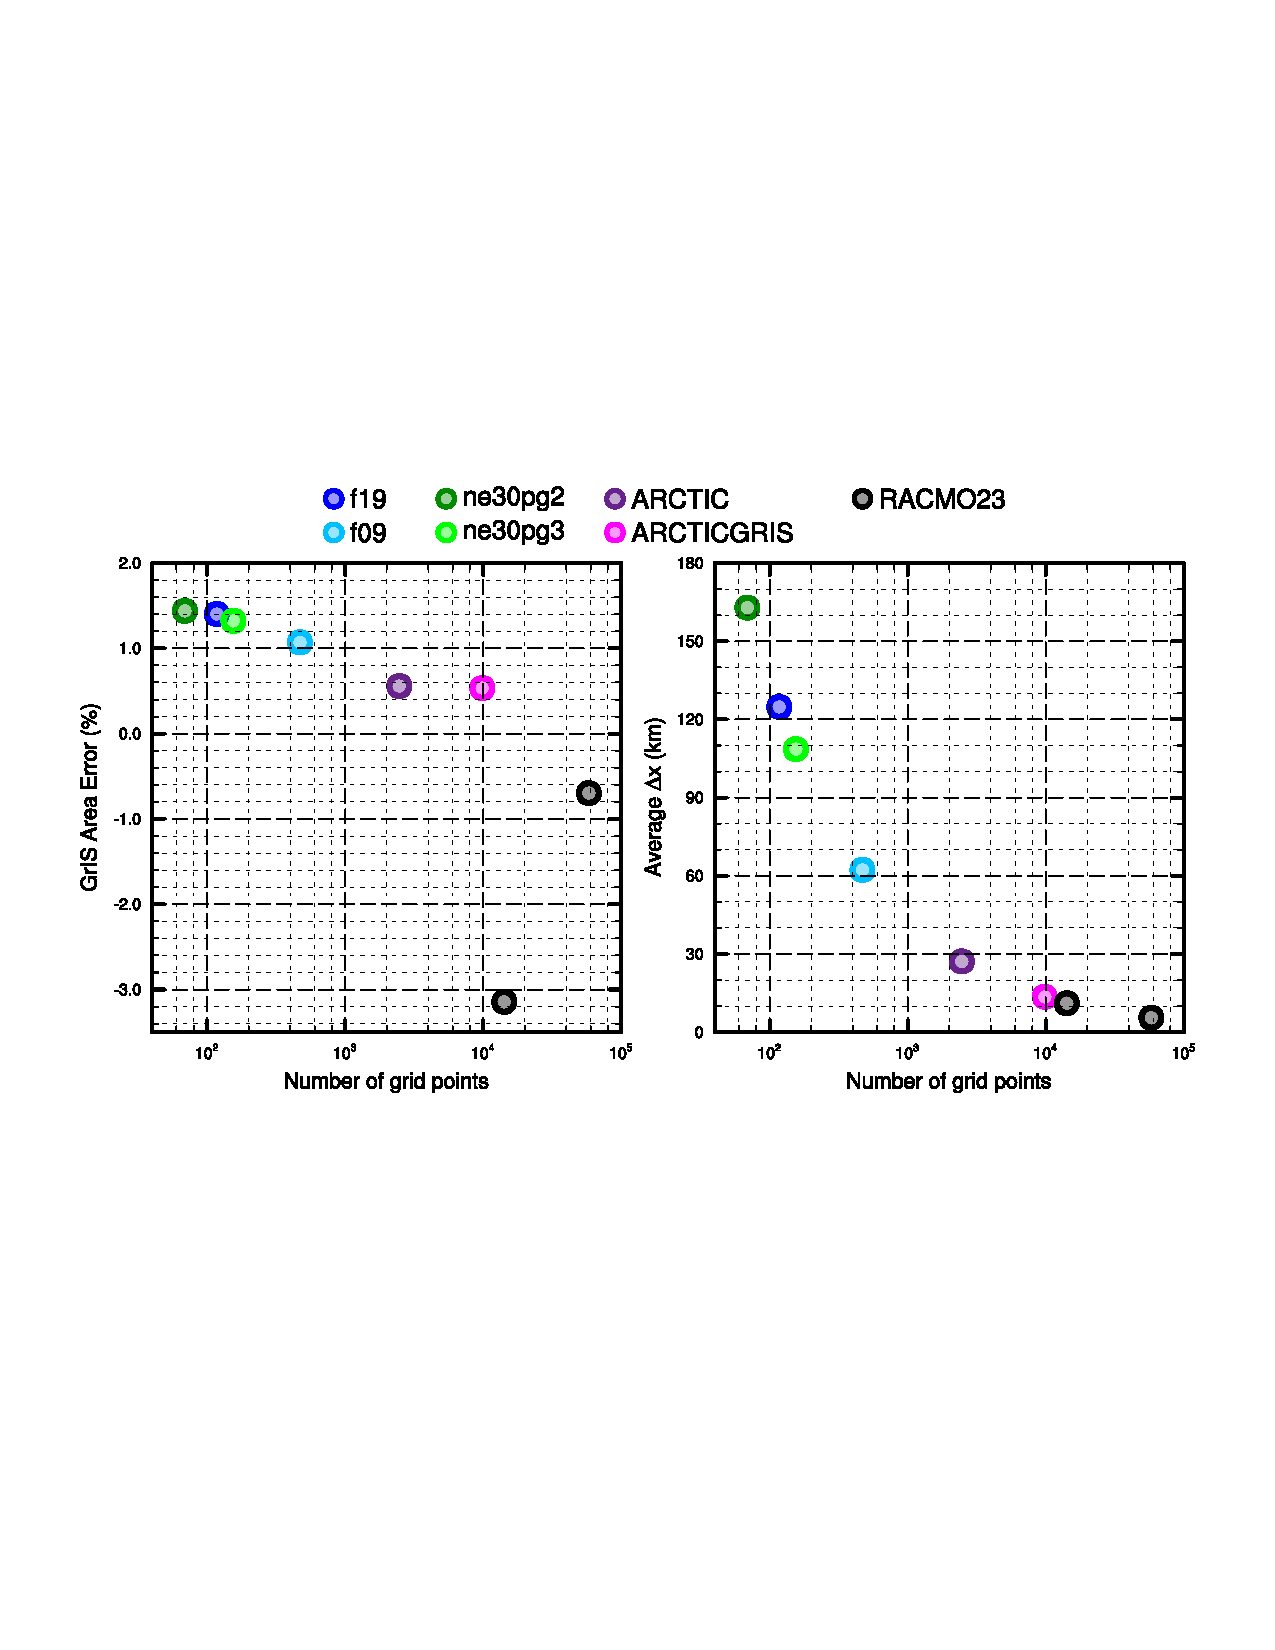
\includegraphics[width=130mm]{figs/temp_grisres.pdf}
\end{center}
\caption{The spatial properties of the GrIS as represented by different grids in this study. (Left) approximate average grid spacing over GrIS, (right) GrIS area error, computed as the relative differences from a 4km dataset used to create the CESM ice masks.}
\label{fig:grisdx}
\end{figure}

\section{Results}\label{sec:results}

\subsection{Tropospheric temperatures}

Before delving into the simulated characteristics of the Arctic, the global mean differences between the various grids and dycores are assessed. Figure~\ref{fig:dT-lores} shows 1979-1998 annual mean, zonal mean height plots expressed as differences between the uniform resolution grids and dycores. The $f09$ grid is warmer than the $f19$ grid, primarily in the mid-to-high latitudes and throughout the depth of the troposphere. This is a common response to increasing horizontal resolution in GCMs \cite{PS2002CD,RETAL2006JC}, and \cite{HK2020QJRMS} has shown that this occurs in CAM due to greater resolved vertical velocities that in turn, facilitate greater condensational heating in the macrophyiscs routine in CLUBB. The right columns in Figure~\ref{fig:dT-lores} supports this interpretation, which shows an increase in the climatological CLUBB heating in the low and mid-latitudes in the $f09$ grid. 

\begin{figure}[t]
\begin{center}
         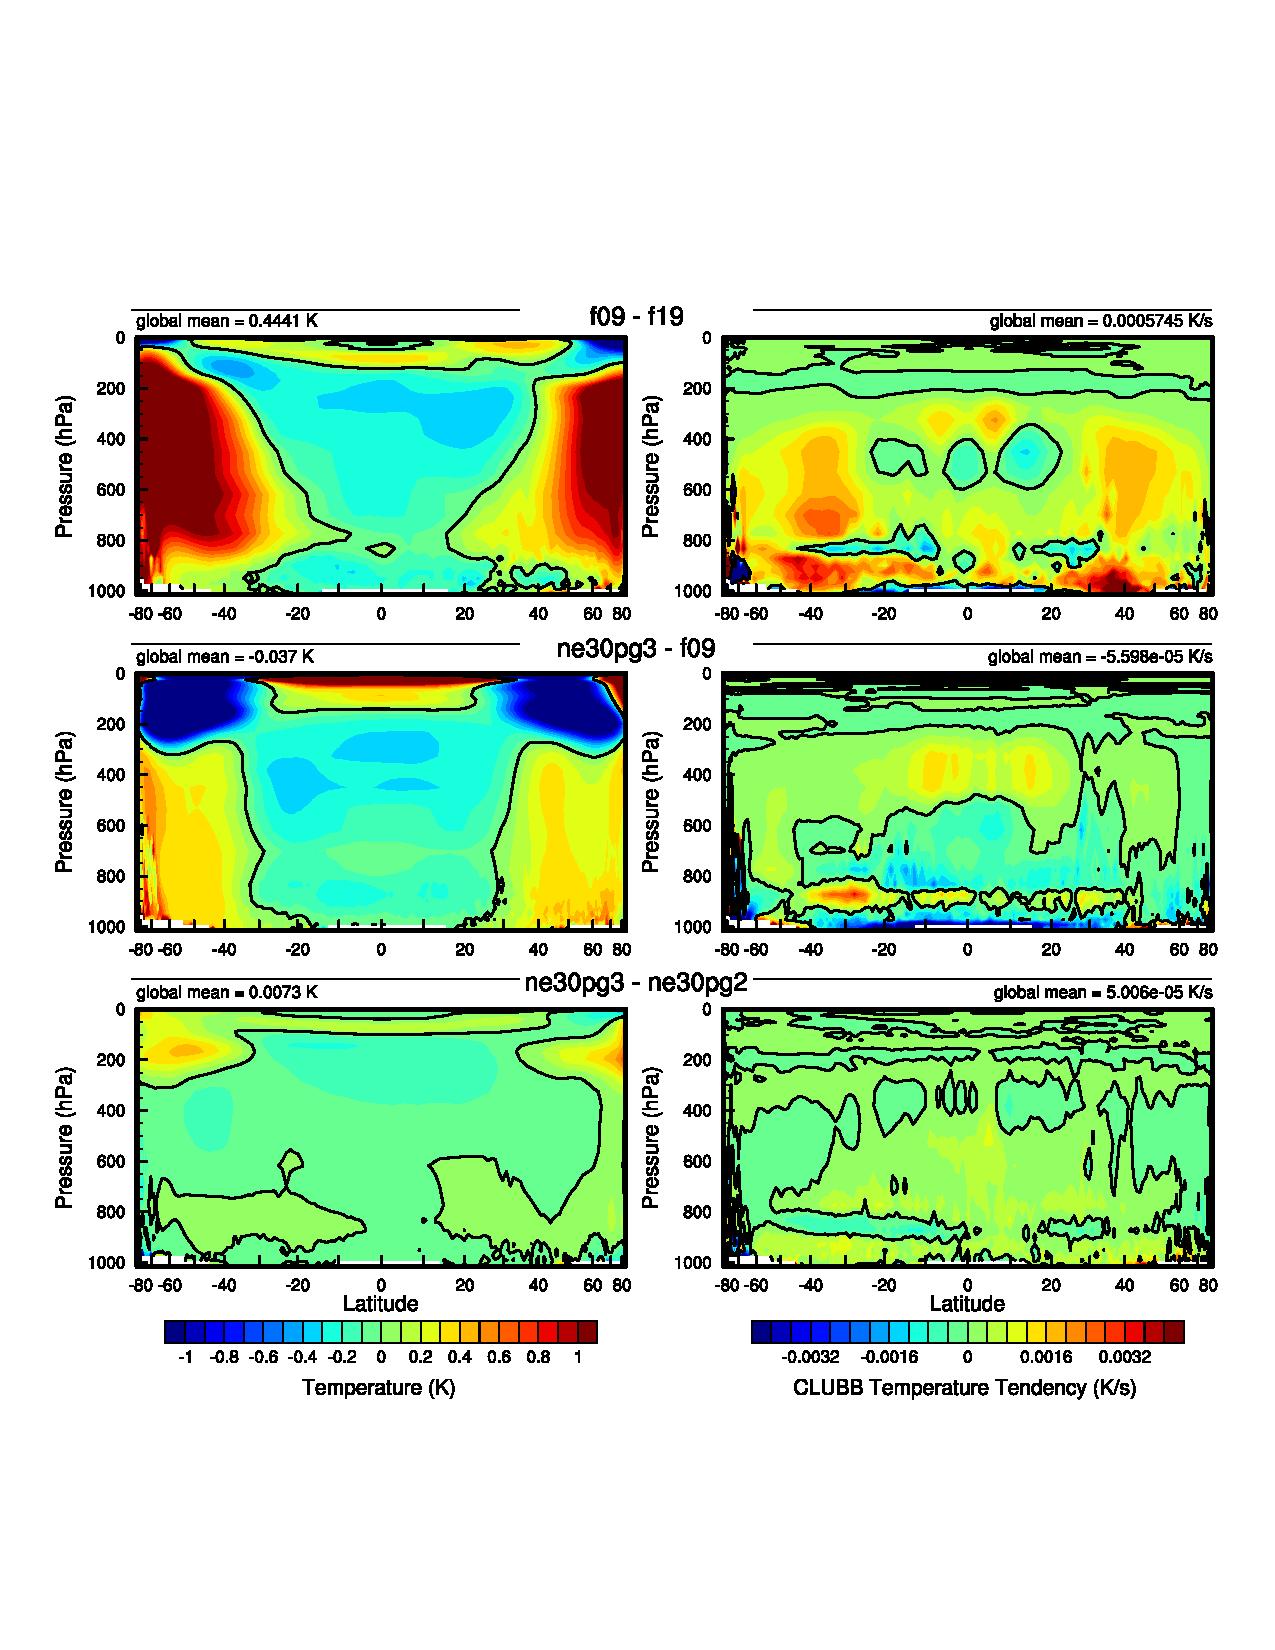
\includegraphics[width=130mm]{figs/temp_dhgt_panel_STEND_CLUBB-lores.pdf}
\end{center}
\caption{.}
\label{fig:dT-lores}
\end{figure}

As the SE dycore is less diffusive than the FV dycore, the resolved vertical velocities are larger in the SE dycore, and so a modest, resolution-like sensitivity occurs in which $ne30pg3$ is warmer than $f09$ (Figure~\ref{fig:dT-lores}). The stratosphere has a different response, in which $ne30pg3$ is much cooler than $f09$ in the mid-to-high latitudes. Figure~\ref{fig:dT-lores} also shows differences in temperature between $ne30pg3$ and $ne30pg2$, which are small, although there is a slight warming near the tropopause at high latitudes. This is consistent with the similar climates found between these grids in \cite{HETAL2019JAMES}.

Comparing the variable-resolution grids to the uniform resolution grids is complicated because we simultaneously increase the grid resolution and reduce the physics time-step, both which noticeably impact the solution \cite{W2008TELLUS}. An additional $ne30pg3$ simulations is run with the physics time-step used in the $ARCTIC$ grid, referred to as $ne30pg3^{*}$. Figure~\ref{fig:dT-hires} shows the change in the climatological summer temperatures in zonal-mean height space between $ne30pg3^{*}$ and $ne30pg3$. A similar warming response to increasing resolution occurs when the time-step is reduced, and the mechanism is similar in that the shorter time-step facilitates greater condensational heating by CLUBB. Figure~\ref{fig:dT-hires} shows the difference in climatological summer temperature between the $ARCTIC$ grid and the $ne30pg3^{*}$ grid. The greater condensational heating and warmer temperatures are confined to the regionally refined region when the impact of physics time-steps is removed from the analysis.

\begin{figure}[t]
\begin{center}
         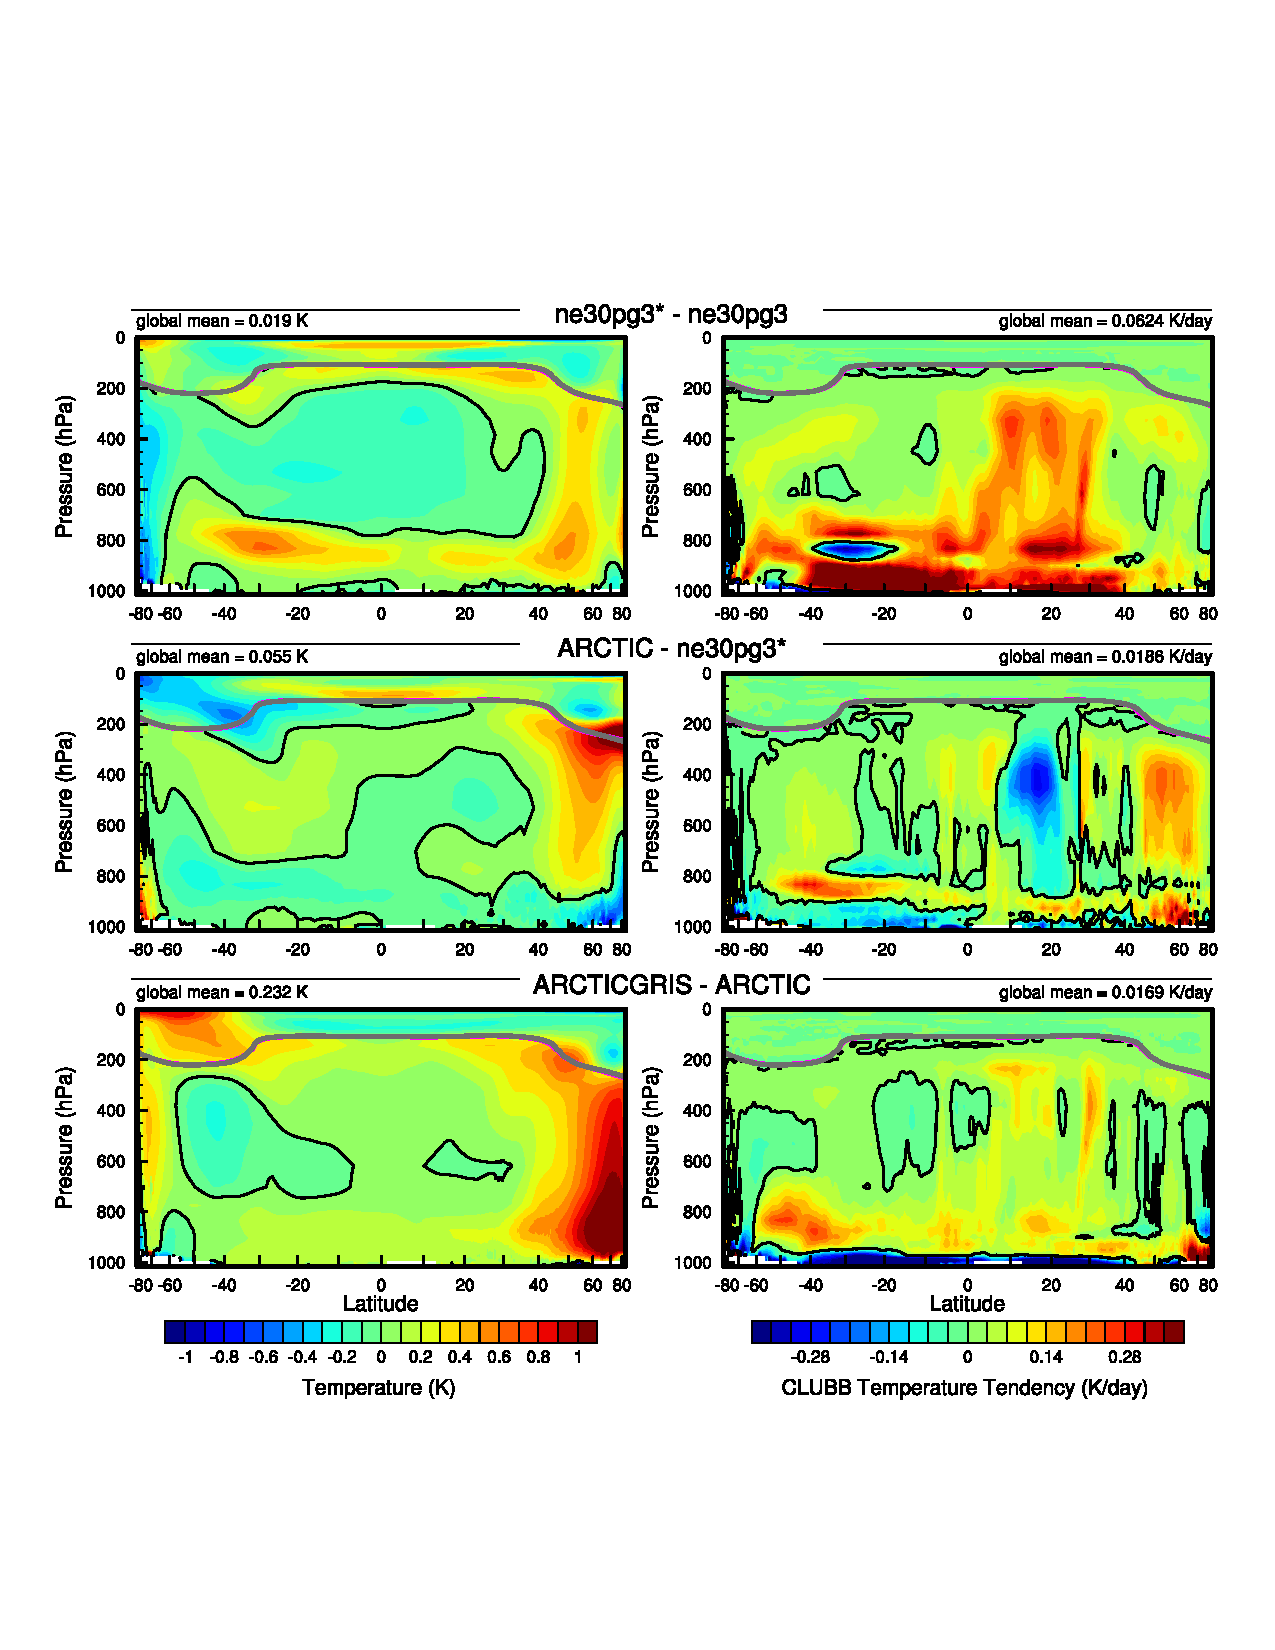
\includegraphics[width=130mm]{figs/temp_dhgt_panel_STEND_CLUBB-hires.pdf}
\end{center}
\caption{.}
\label{fig:dT-hires}
\end{figure}

It's useful to understand summer temperature biases, instead of annual means, due to its control on ice/snow melt \cite{O2001JAM,HT2008Paleo}. Figure~\ref{fig:dThyps} shows the 1979-1998 lower troposphere summer temperature bias relative to ERA5. It is computed from the 500 hPa-1000 hPa geopotential thickness, solving for the layer mean virtual temperature using the hypsometric equation. The results generally track with the analysis of the zonal mean height plots; increasing resolution from $f19$ to $f09$ leads to a warmer climate, and the $1^{\circ}$ spectral-elements grids are warmer than the finite-volume grids. The summer temperatures in the finite-volume grids are persistently colder than ERA5 at high latitudes, whereas the $1^{\circ}$ spectral-element grids are warmer than ERA5 at only very high-latitudes, north of $80^{\circ}$. All grid illustrate a north-south gradient in bias over Greenland, in which the summer temperature bias becomes more positive in the northward direction. This pattern is also evident in the 2m summer temperature bias over Greenland (not shown).

The $ARCTIC$ grid has similar summer temperatures to the $1^{\circ}$ spectral-element grids, but it is a bit warmer over northern Eurasia and the North Pole. An anomalous cooling patch forms to the west of Greenland, centered over Baffin Island. The $ARCTICGRIS$ grid is warmer than the $ARCTIC$ grid over most of the Arctic region, but approximately maintains the same pattern of summer temperature bias as in the $ARCTIC$ grid.

Some of these temperature anomalies may be related to summer shortwave cloud forcing differences across the different grids and dycores. Figure~\ref{fig:SWCF} shows the summer short-wave cloud forcing bias in the runs, using the CERES-EBAF product. All the uniform $1^{\circ}-2^{\circ}$ grids have similar biases, with the clouds reflecting 20-40 W/m2 too much shortwave radiation over a wide swath of the Arctic, primarily over the land masses. There's also a halo of low cloud forcing bias around the oceanic perimeter of Greenland. The $ARCTIC$ grid has much smaller cloud forcing biases over the Arctic land masses, although still too reflective, whereas the $ARCTCGRIS$ grid vastly improves the cloud forcing bias over Eurasia, and improves the bias over N.America compared to the $ARCTIC$ grid. In both variable-resolution grids, the halo of too weak cloud forcing bias around the perimeter of Greenland is absent.

While the summer cloud forcing biases are consistent with the summer temperature biases in Figure~\ref{fig:dThyps} --regions where clouds are too reflective coincide with regions that are too cold-- it is not clear whether the cold biases are caused by the cloud biases, or whether the cold biases amplify the cloud forcing bias.

\begin{figure}[t]
\begin{center}
         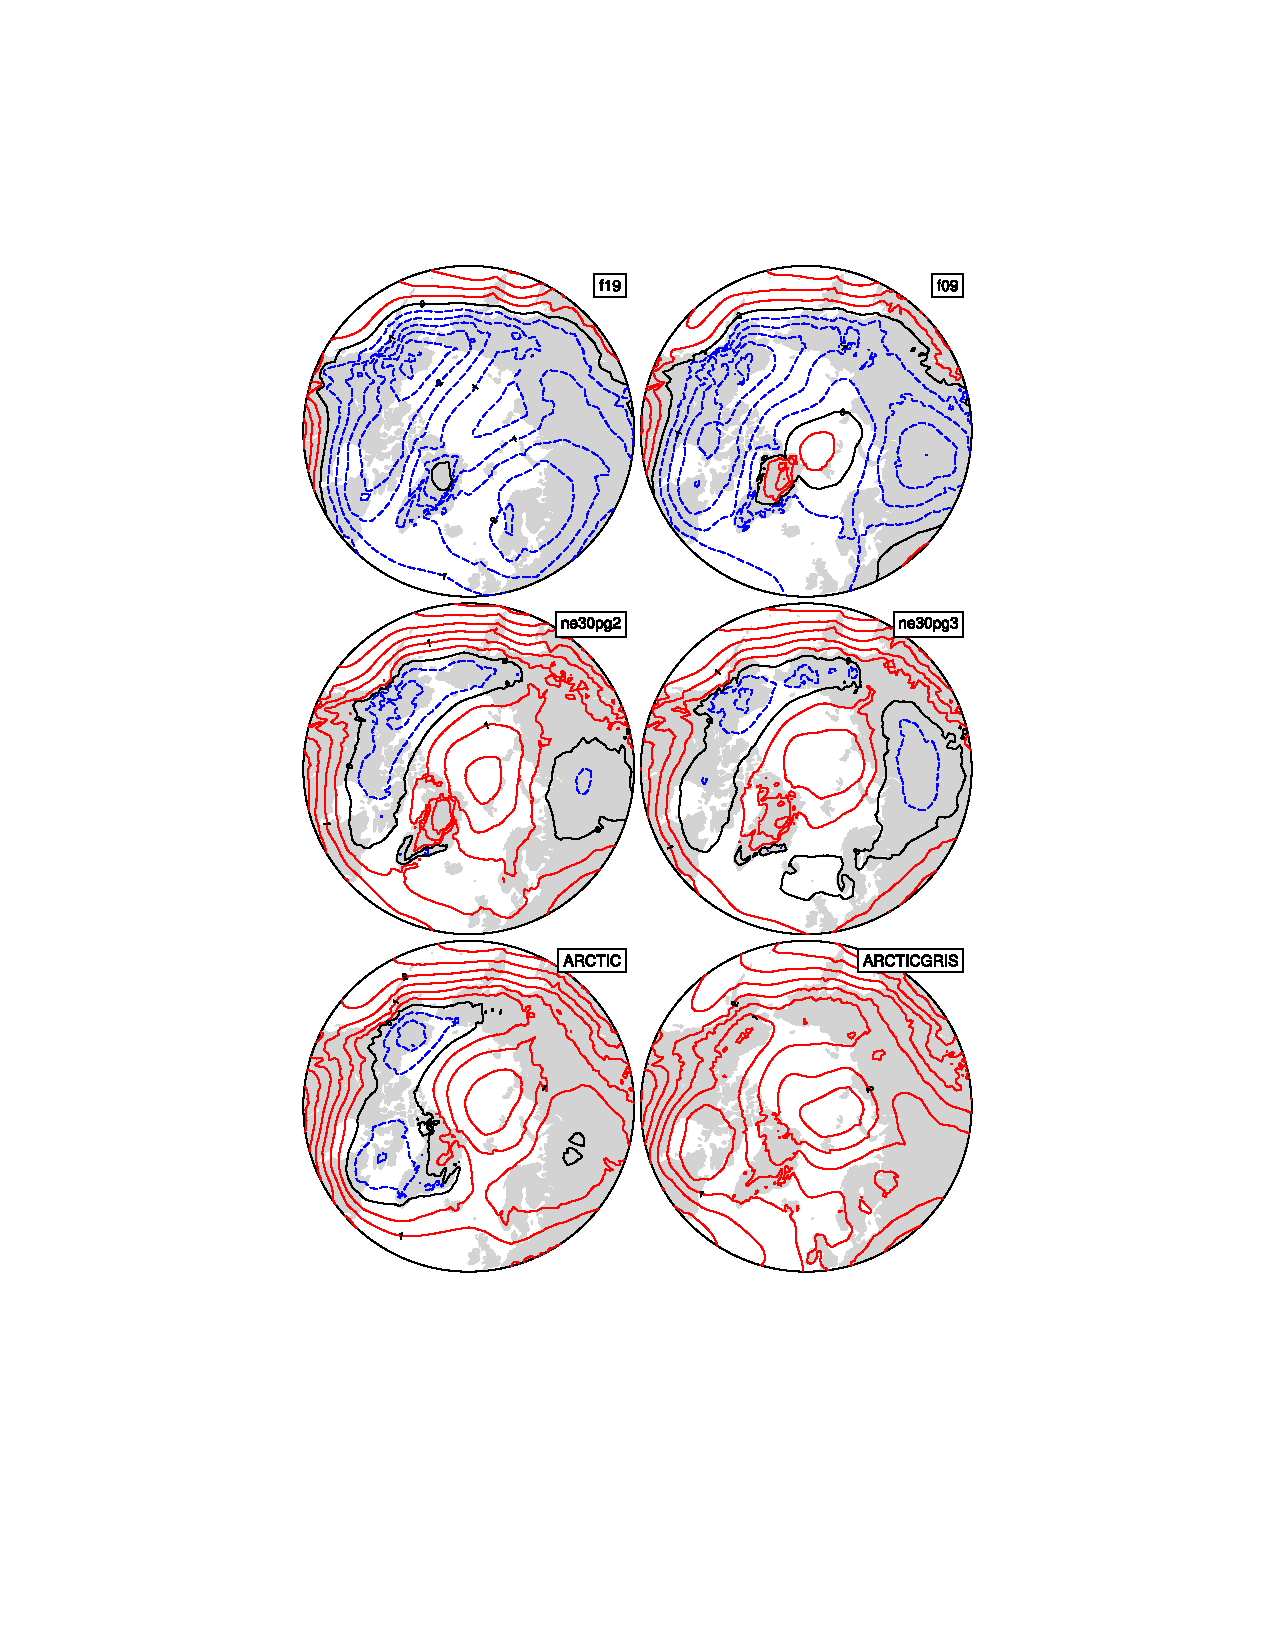
\includegraphics[width=100mm]{figs/temp_contours_diffERA5_Thyps.pdf}
\end{center}
\caption{.}
\label{fig:dThyps}
\end{figure}

\begin{figure}[t]
\begin{center}
         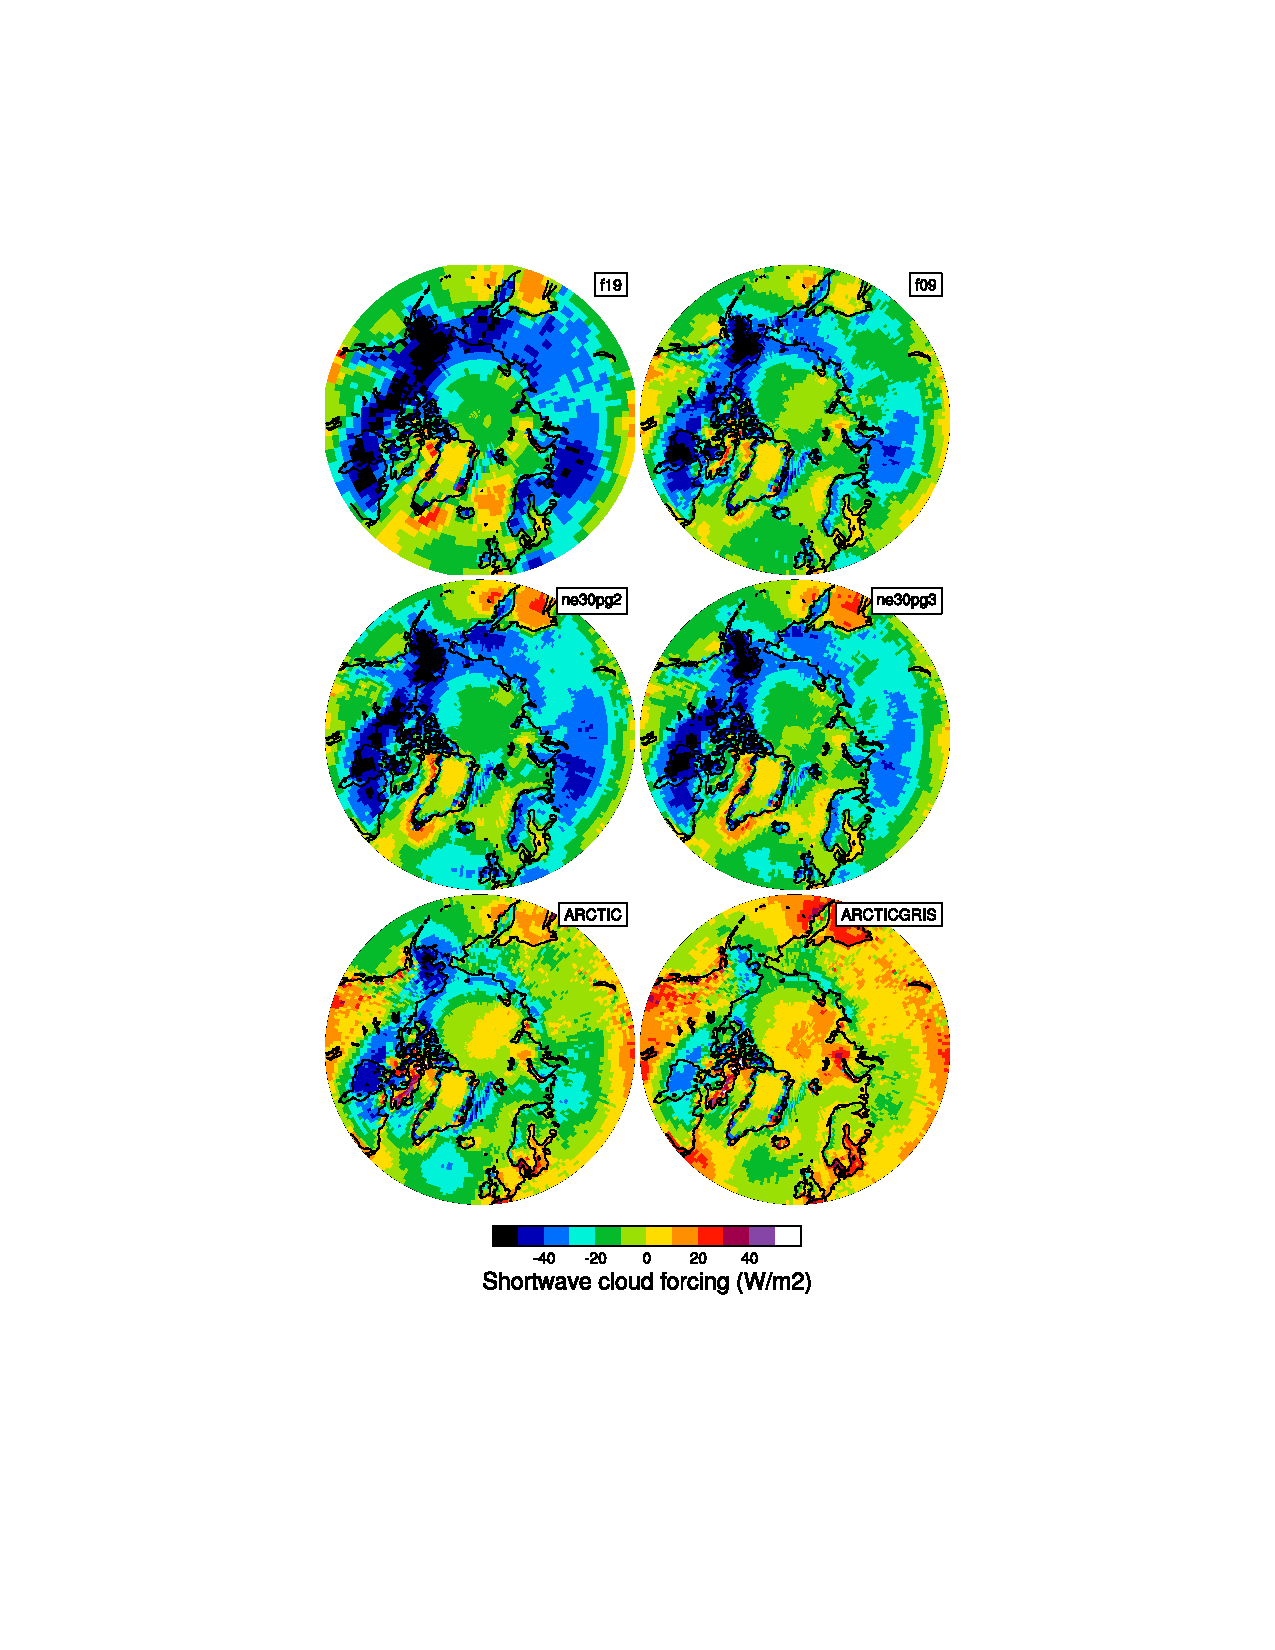
\includegraphics[width=100mm]{figs/temp_contours_diffCERES_SWCF.pdf}
\end{center}
\caption{.}
\label{fig:SWCF}
\end{figure}

\subsection{Shortwave radiation over Greenland}

In addition to summer temperatures, shortwave radiation is also an important determinant of snow/ice melt. Figure~\ref{fig:FSDS} shows the summer incident shortwave radiation bias at the surface, zoomed in over Greenland. The top panel computes the bias using the CERES-EBAF dataset, and the bottom panel using RACMO2.3p2 dataset.
This halo of excessive incident shortwave radiation around the coasts of Greenland is apparent in both datasets, consistent with the shortwave cloud forcing biases in Figure~\ref{fig:SWCF}.

The interior of the ice sheet receives too little shortwave radiation in the coarser grids. In the variable-resolution grids, both the interior deficit in shortwave and the excessive shortwave around the oceanic perimeter of Greenland are improved. This suggests that the coarse grids clouds are too thick in the interior of Greenland, and too thin around the perimeter of Greenland, and that increasing horizontal resolution balances out these biases. This is consistent with total summer cloud fraction bias, computed from the CALIPSO cloud dataset (Figure~\ref{fig:prect}). Note that total cloud fraction characterizes the cloud field at all vertical levels, but attenuates any changes arising from any single layer due to the maximum overlap assumption used to compute this quantity. Despite the attenuated signal, the total cloud fraction does indicate a reduction in cloud coverage in the interior, and an increase in cloudiness about the oceanic perimeter, in the variable-resolution grids. 

The agreement of the cloud biases over Greenland in multiple independent datasets indicates this is a robust feature of the coarser grids. The reduction of these cloud biases in the variable-resolution grids suggests they are a result of insufficient horizontal resolution in coarse grids.

\begin{figure}[t]
\begin{center}
         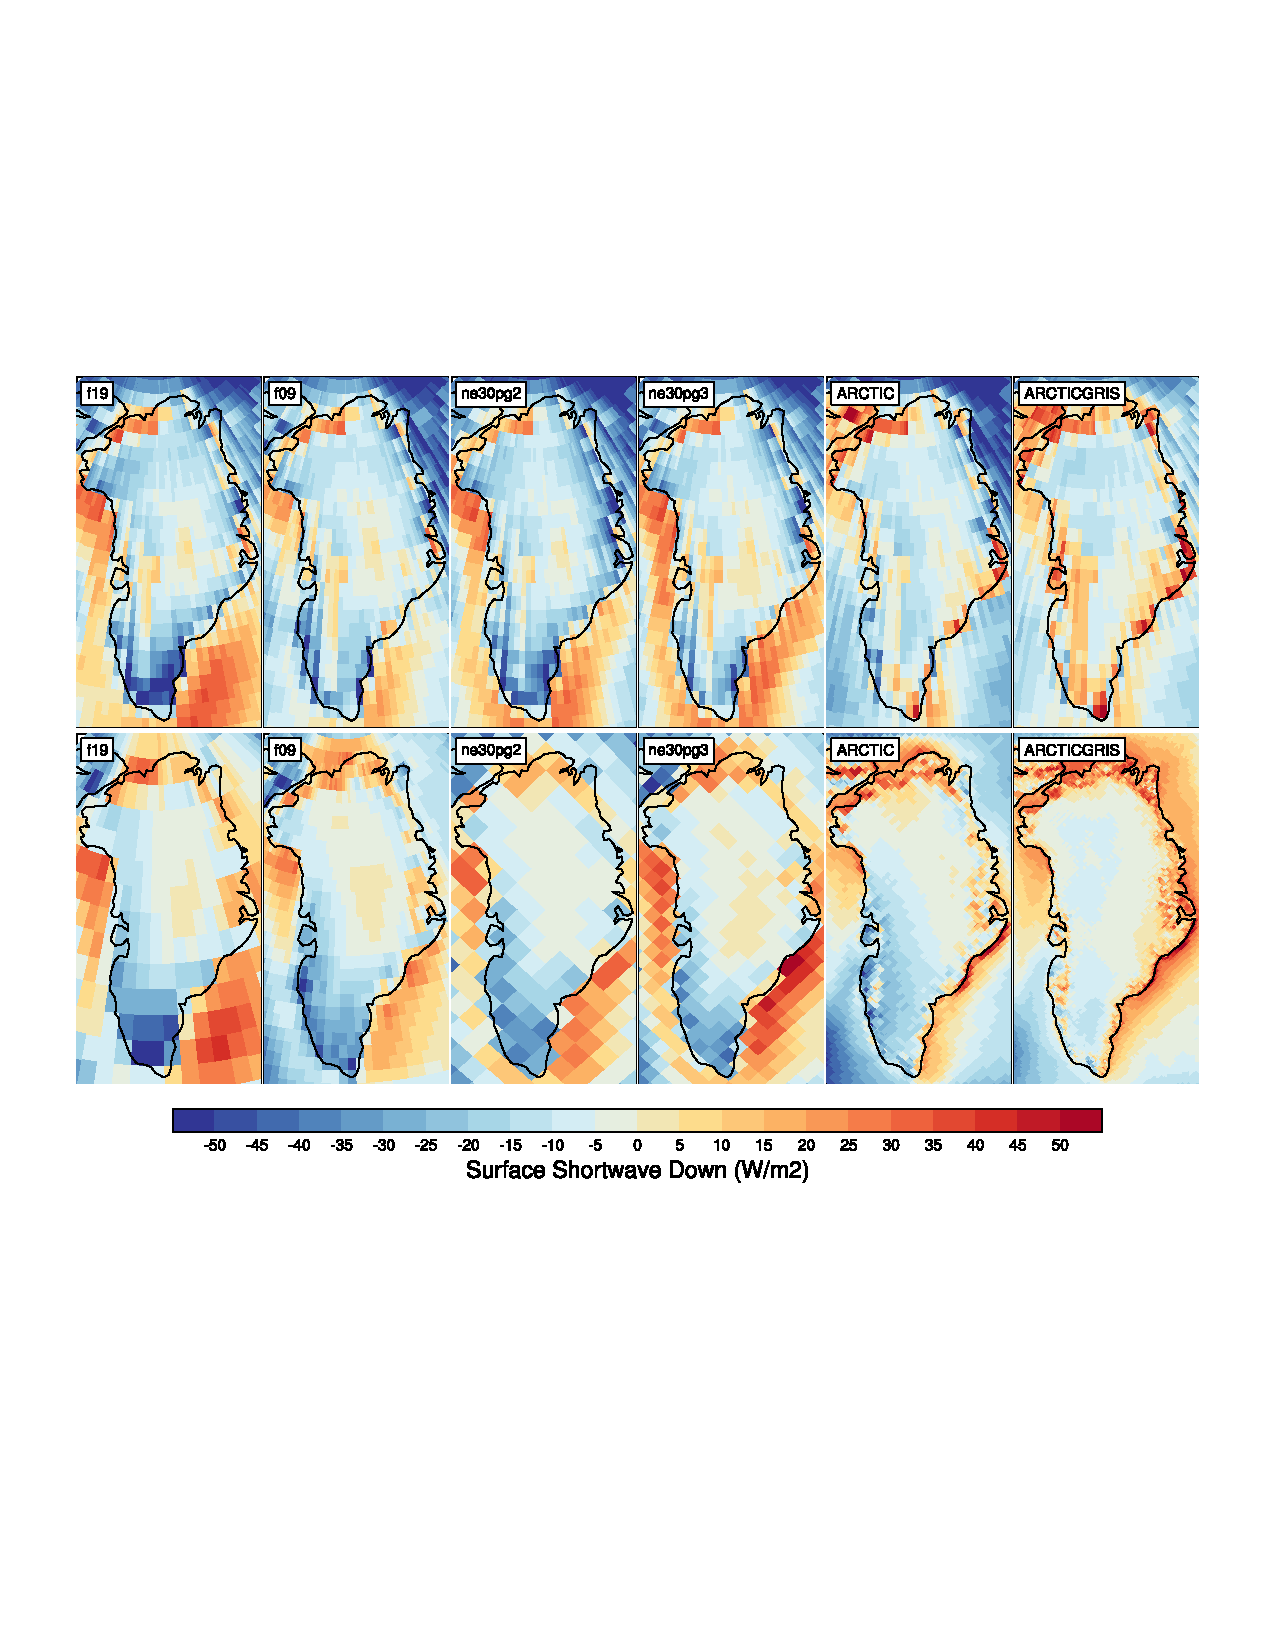
\includegraphics[width=130mm]{figs/temp_contours_diffCERESdiffRACMO_FSDS.pdf}
\end{center}
\caption{.}
\label{fig:FSDS}
\end{figure}

\begin{figure}[t]
\begin{center}
         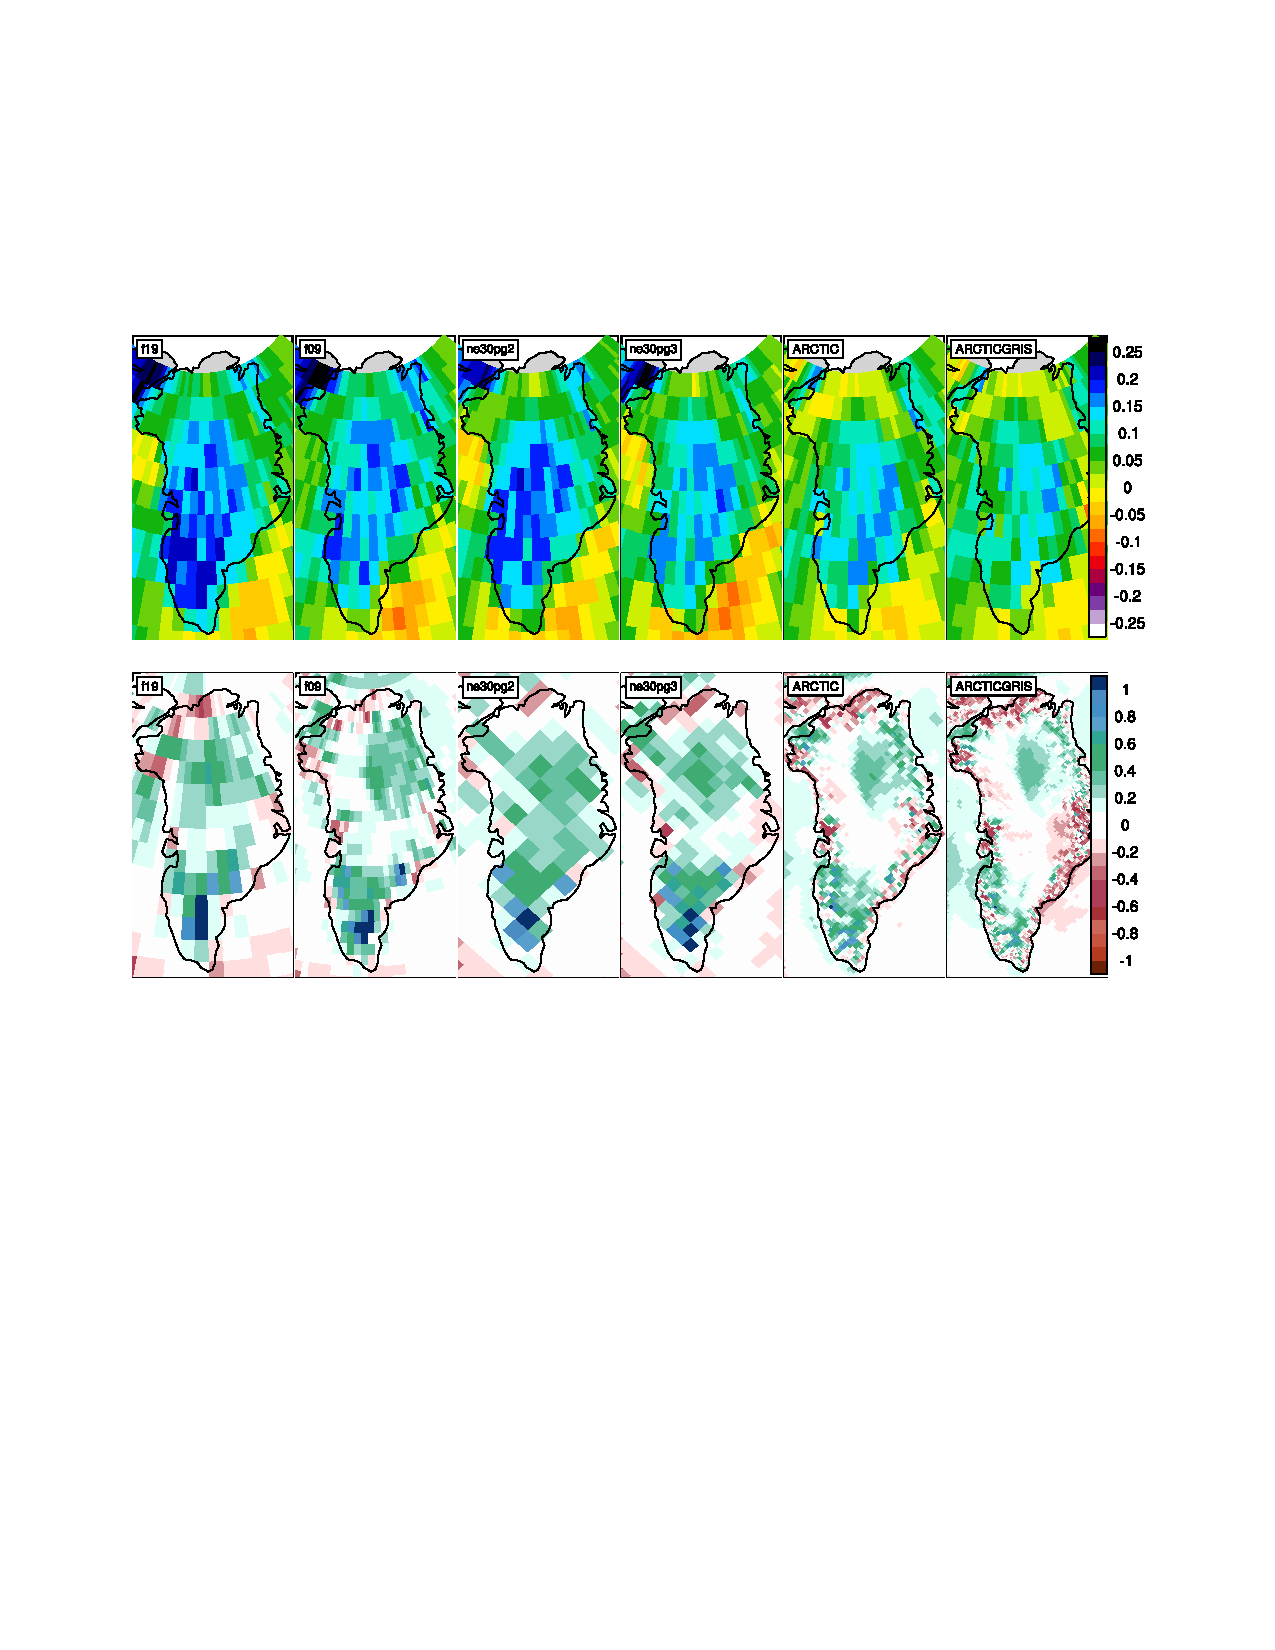
\includegraphics[width=130mm]{figs/temp_contours_diffCERESdiffRACMO_CLOUD_PRECIP.pdf}
\end{center}
\caption{Climatological (1979-1998) annual precipitation rate bias (in mm/yr) relative to the RACMO2.3p2 5.5km resolution data product \cite{NETAL2019SCIENCE}.}
\label{fig:prect}
\end{figure}

\subsection{Greenland surface mass balance}

The accuracy of the simulated SMB is expected to be sensitive to grid resolution. Figure~\ref{fig:prect} shows the average grid spacing over the Greenland Ice Sheet (GrIS) in all six grids in this study. The $ne30pg2$ grid has the coarsest representation with an average $\Delta x=160~km$, and the $ARCTICGRIS$ grid has the highest resolution with an average $\Delta x=14.6~km$, similar to the grid spacing of the $11~km$ RACMO2.3 grid. The $ne30pg3$ grid has an average $\Delta x=111.2~km$, which is substantially more coarse than the $f09$ grid, with an average $\Delta x=60~km$. This is interesting because $ne30pg3$ and $f09$ have similar average grid spacing over the entire globe, and comparable computational costs, but due to the convergence of meridians the finite-volume model has enhanced resolution over GrIS. The $ARCTIC$ grid has an average grid spacing of $\Delta x=27.8~km$, and is about 10 times more expensive than the $1^{\circ}$ models (whereas the $ARCTICGRIS$ grid is about twice as expensive as the $ARCTIC$ grid).

The summer climatological mean precipitation bias over GrIS is shown in Figure~\ref{fig:grisdx}, expressed as the fractional difference from the RACMO2.3p2 solution. What sticks out is that the coarse $1^{\circ}-2^{\circ}$ grids have large, positive biases centered over the southern dome. The $ARCTIC$ run improves this bias substantially, and the $ARCTICGIS$ run improves this bias further. This suggests the southern dome bias is due to inadequate horizontal resolution, which is consistent with the original GrIS variable-resolution experiments in \cite{VETAL2018TC}. 

Southeast Greenland has the largest accumulation rates in GrIS due to synoptic systems moving in from the southeast. These systems are orographically lifted by the steep southeast ice sheet margin, dumping large amounts of precipitation along the southeast coast. At lower horizontal resolutions, the topography is too smooth and large amounts of moisture penetrates further inland, incorrectly dumping precipitation onto the interior of the ice sheet. A similar bias occurs in northwest Greenland, in particular during the summer, when it's common for synoptic systems to arrive from the southwest. The ability of the variable-resolution grids to more accurately simulate the orographic precipitation process in Greenland is consistent with all the cloud results up to this point. Since the precipitation centers move from the interior towards the coasts, and even out over the ocean with increasing resolution, the cloud decks should, and are, moved accordingly, eliminating this halo of low cloud bias around the oceanic perimeter of Greenland.

Figure~\ref{fig:tseries} shows time-series of annually integrated precipitation and snow/ice melt over the GrIS in the various different grids and dycores, with both versions of RACMO shown in black. The 1979-1998 climatological mean values are provided as circles on the right side of the panels. The uniform $1^{\circ}-2^{\circ}$ grids all show a distinctive positive bias in precipitation due to this over-prediction of interior precipitation rates. The  variable-resolution grids have the smallest precipitation biases, providing a comparable solution to RACMO.The $f19$ and $f09$ perform similarly, with +110 Gt/yr bias, whereas $ne30pg3$ is biased by about +165 Gt/yr and $ne30pg2$, +230 Gt/yr. The results suggest that uniform resolution spectral-element grids have larger biases than the finite-volume grids, consistent with spectral-element grids having a coarser representation of GrIS (Figure~\ref{fig:grisdx}).

The combined annual snow/ice melt integrated over the GrIS is given by the bottom panel of Figure~\ref{fig:tseries}. The $ARCTIC$ grid simulates the most realistic melt rates, with all other grids tending to have larger melt rates than RACMO. The $ARCTICGRIS$ grid over predicts melting by about 125 Gt/yr. This is likely due to an anomalously warm lower troposphere during the summer, relative to the $ARCTIC$ run (Figure~\ref{fig:dThyps}). The $f19$ and $f09$ melting rates are improved over $ARCTICGRIS$, simulating too much melt by about 70-90 Gt/yr. The spectral-element grids have the largest positive melt bias, between 200-220 Gt/yr. It is more difficult to attribute these differences to resolution alone, since the finite-volumes grids have colder summer temperatures than the uniform resolution spectral-element grids. However, that the $ARCTCIGRIS$ grid has the warmest summer temperatures, yet has a lower melting bias than the uniform spectral-element grids, suggests that increasing resolution improves the ablation process.

 \begin{table*}
 \centering
 \scriptsize
 \begin{tabular}{lccc}
   \hline
   grid name & accumulation (Gt/yr) & ice/snow melt (Gt/yr) \\ 
   \hline
   $RACMO$ & 768.5 & -347.2 \\
   \hline
   $f19$ & 882.5 & -440.3 \\
   $f09$ & 874.8 & -418.4 \\
   $ne30pg2$ & 1000. & -549.4 \\
   $ne30pg3$ & 934.9 & -568.8 \\
   $ARCTIC$ & 795.9 & -367.3 \\
   $ARCTICGRIS$ & 708.7 & -471.6 \\
 \hline
 \end{tabular}
  \caption{1979-1998 Surface Mass Balance of the Greenland Ice Sheet.}
 \label{tbl:table3}
 \end{table*}

\begin{figure}[t]
\begin{center}
         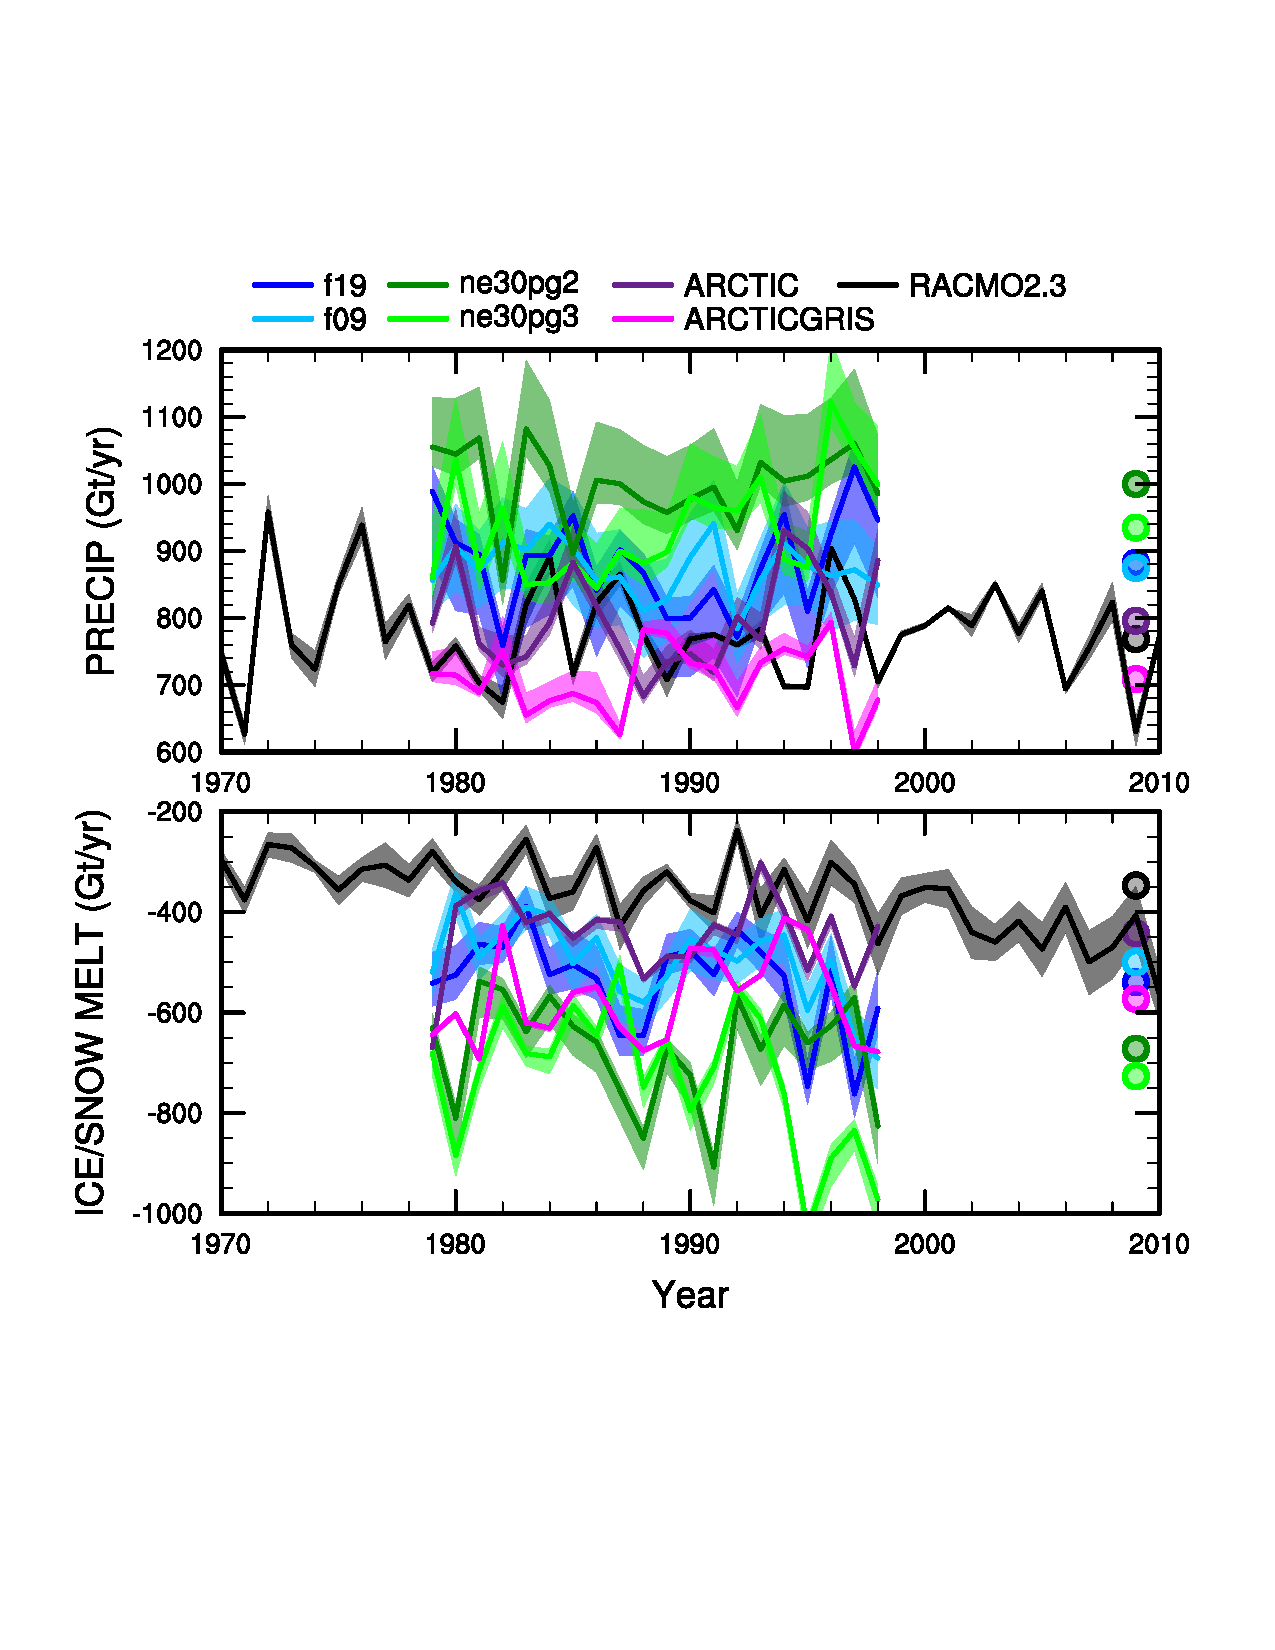
\includegraphics[width=100mm]{figs/temp_tseries_GRIS.pdf}
\end{center}
\caption{Time-series of annual (solid+liquid) precipitation (top) and annual runoff (bottom) integrated over the Greenland Ice Sheet for all six simulations and compared to RACMO3.2. The raw fields are mapped to two target low resolution grids, f19 \& ne30pg2, and using two different remapping methods, conservative ESMF and high order TempestRemap. The remapped values are then integrated over the ice mask of the target grid. This gives four time-series for each simulation (three for f19 \& ne30pg2), with the mean value given by the solid line and shading spanning the extent of the remapped solutions.}
\label{fig:tseries}
\end{figure}

\begin{figure}[t]
\begin{center}
         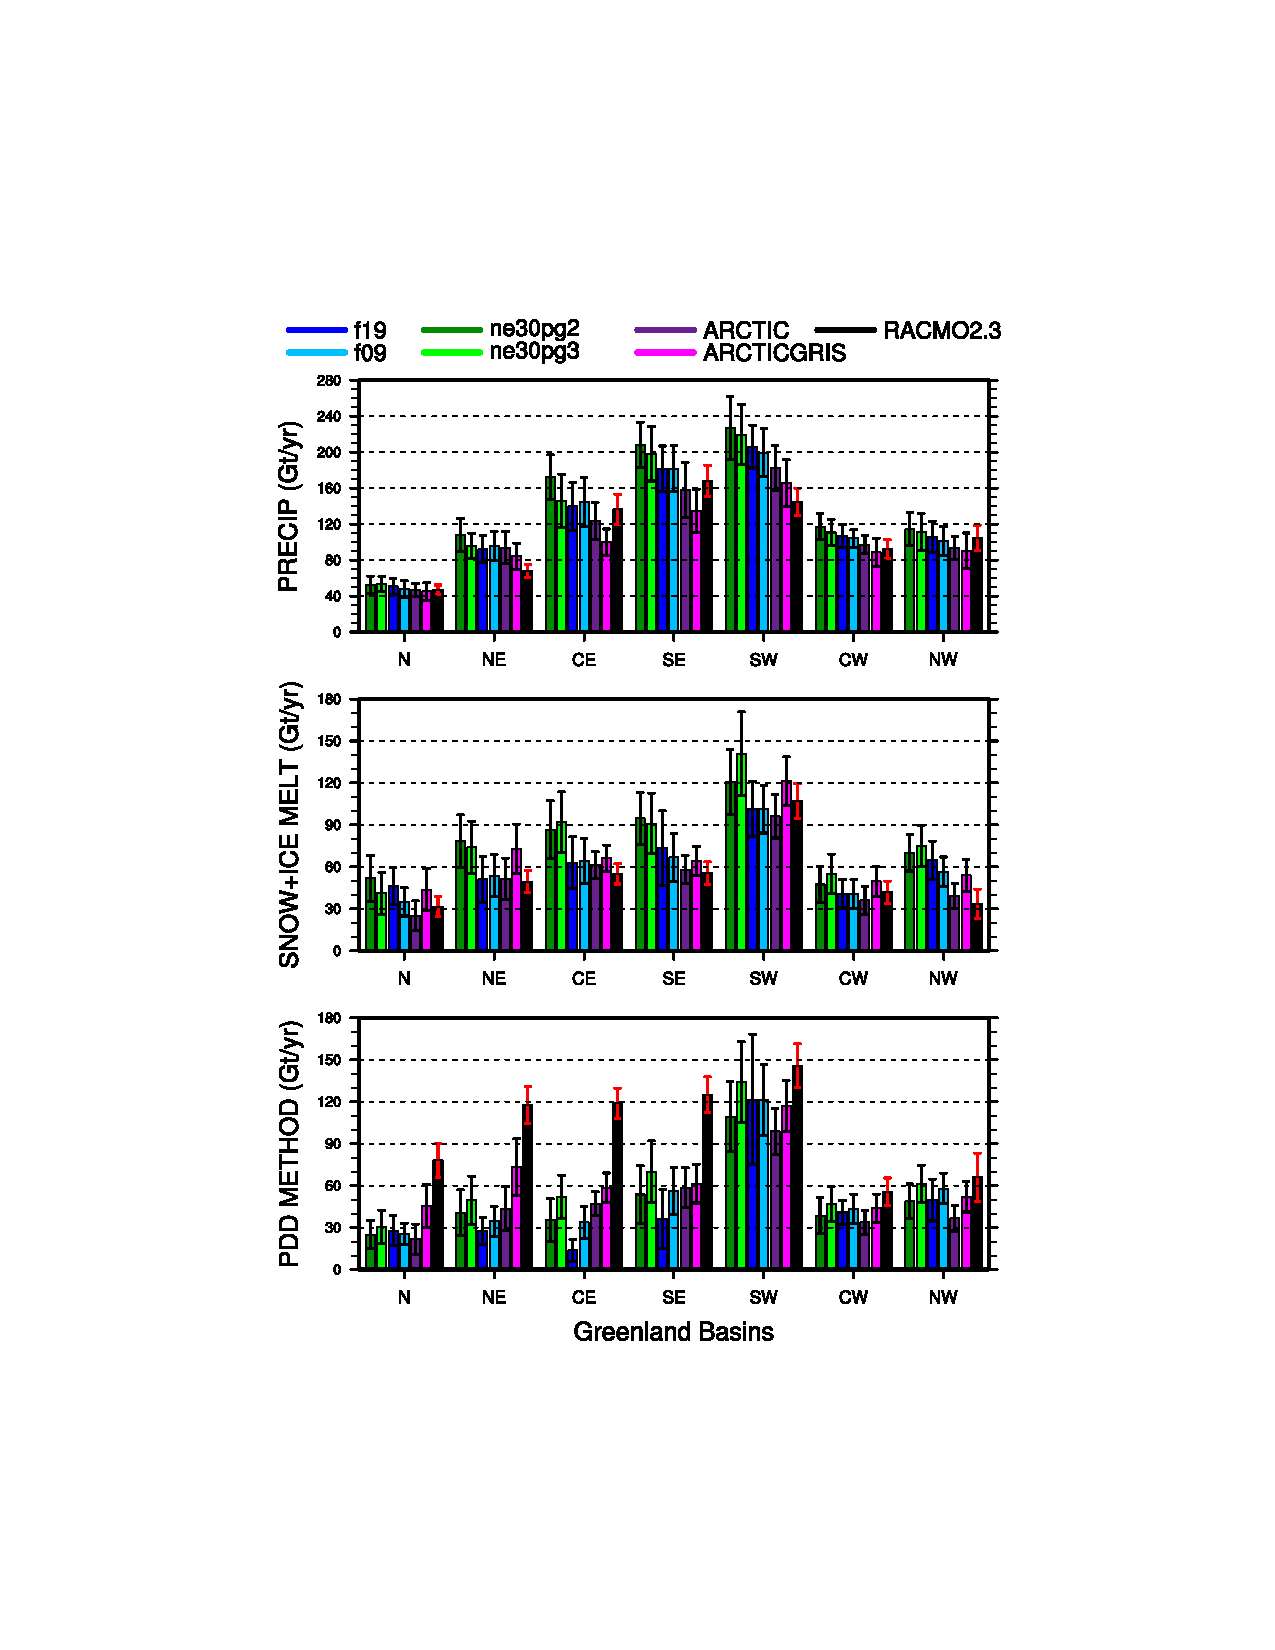
\includegraphics[width=100mm]{figs/temp_tseries_BASIN.pdf}
\end{center}
\caption{.}
\label{fig:basin}
\end{figure}

\begin{figure}[t]
\begin{center}
         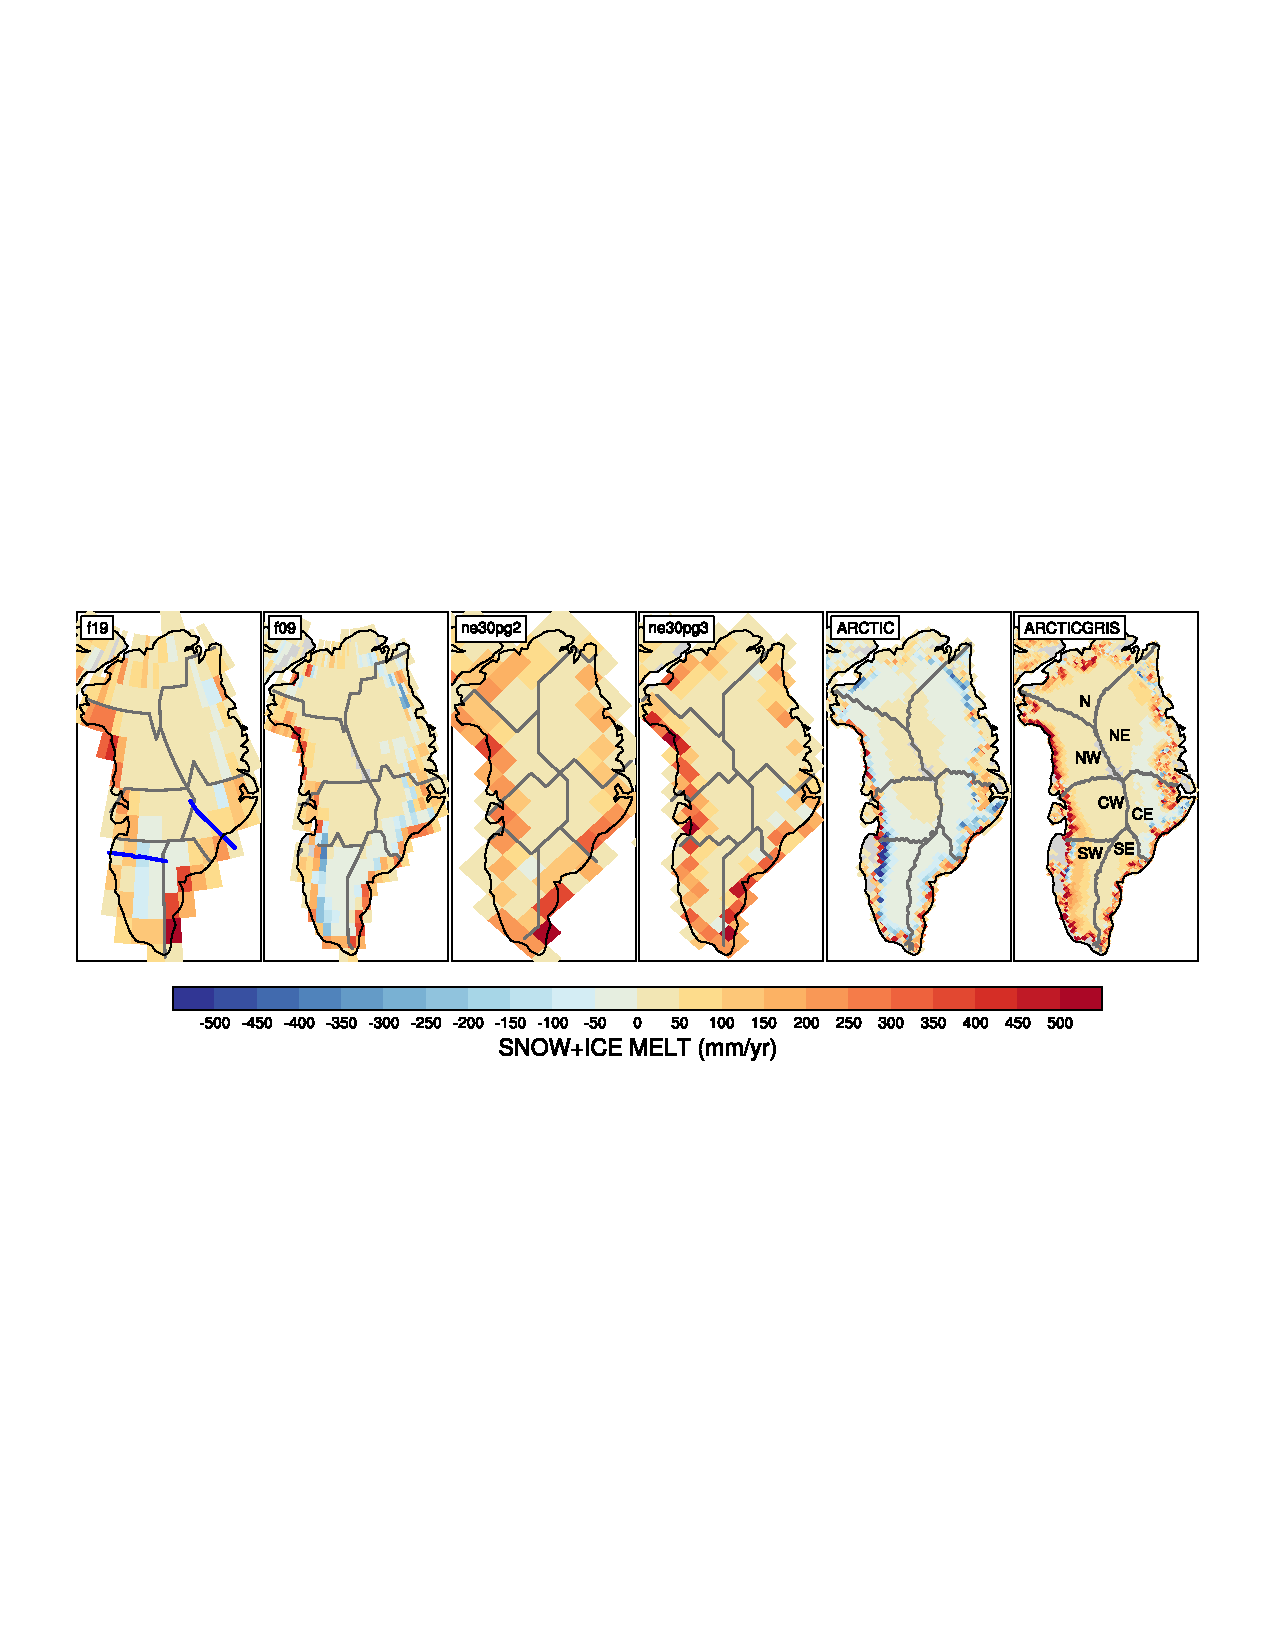
\includegraphics[width=130mm]{figs/temp_contours_diffRACMO_melt.pdf}
\end{center}
\caption{.}
\label{fig:melt}
\end{figure}

Figure~\ref{fig:pointdiff} shows the distribution of point-wise differences from LIVVkit observational database as violin plots. The IceBridge dataset is exclusively from the interior of the ice sheet and represents accumulation rates. The uniform $1^{\circ}-2^{\circ}$ grids have similar median errors of about +35-50 mm.w.e, while the variable-resolution errors are noticeably smaller. The in-situ observations in the accumulation zone, shown in the middle plot looks very similar to the IceBridge errors, providing confidence that the variable-resolution grids are outperforming the uniform grids in the interior accumulation zone. The errors evaluated at in-situ ablation zone measurements are in tension with the RACMO results in Figure~\ref{fig:tseries}. They indicate that the uniform $1^{\circ}-2^{\circ}$ grids perform similarly, and that the $ARCTICGRIS$ performs best, and an improvement over the $ARCTIC$ grid. However, the in-situ ablation measurements are sparse in time and space, and so there is a large amount of uncertainty in extending these results to the entirety of the ablation zone.

%\begin{figure}[t]
%\begin{center}
%         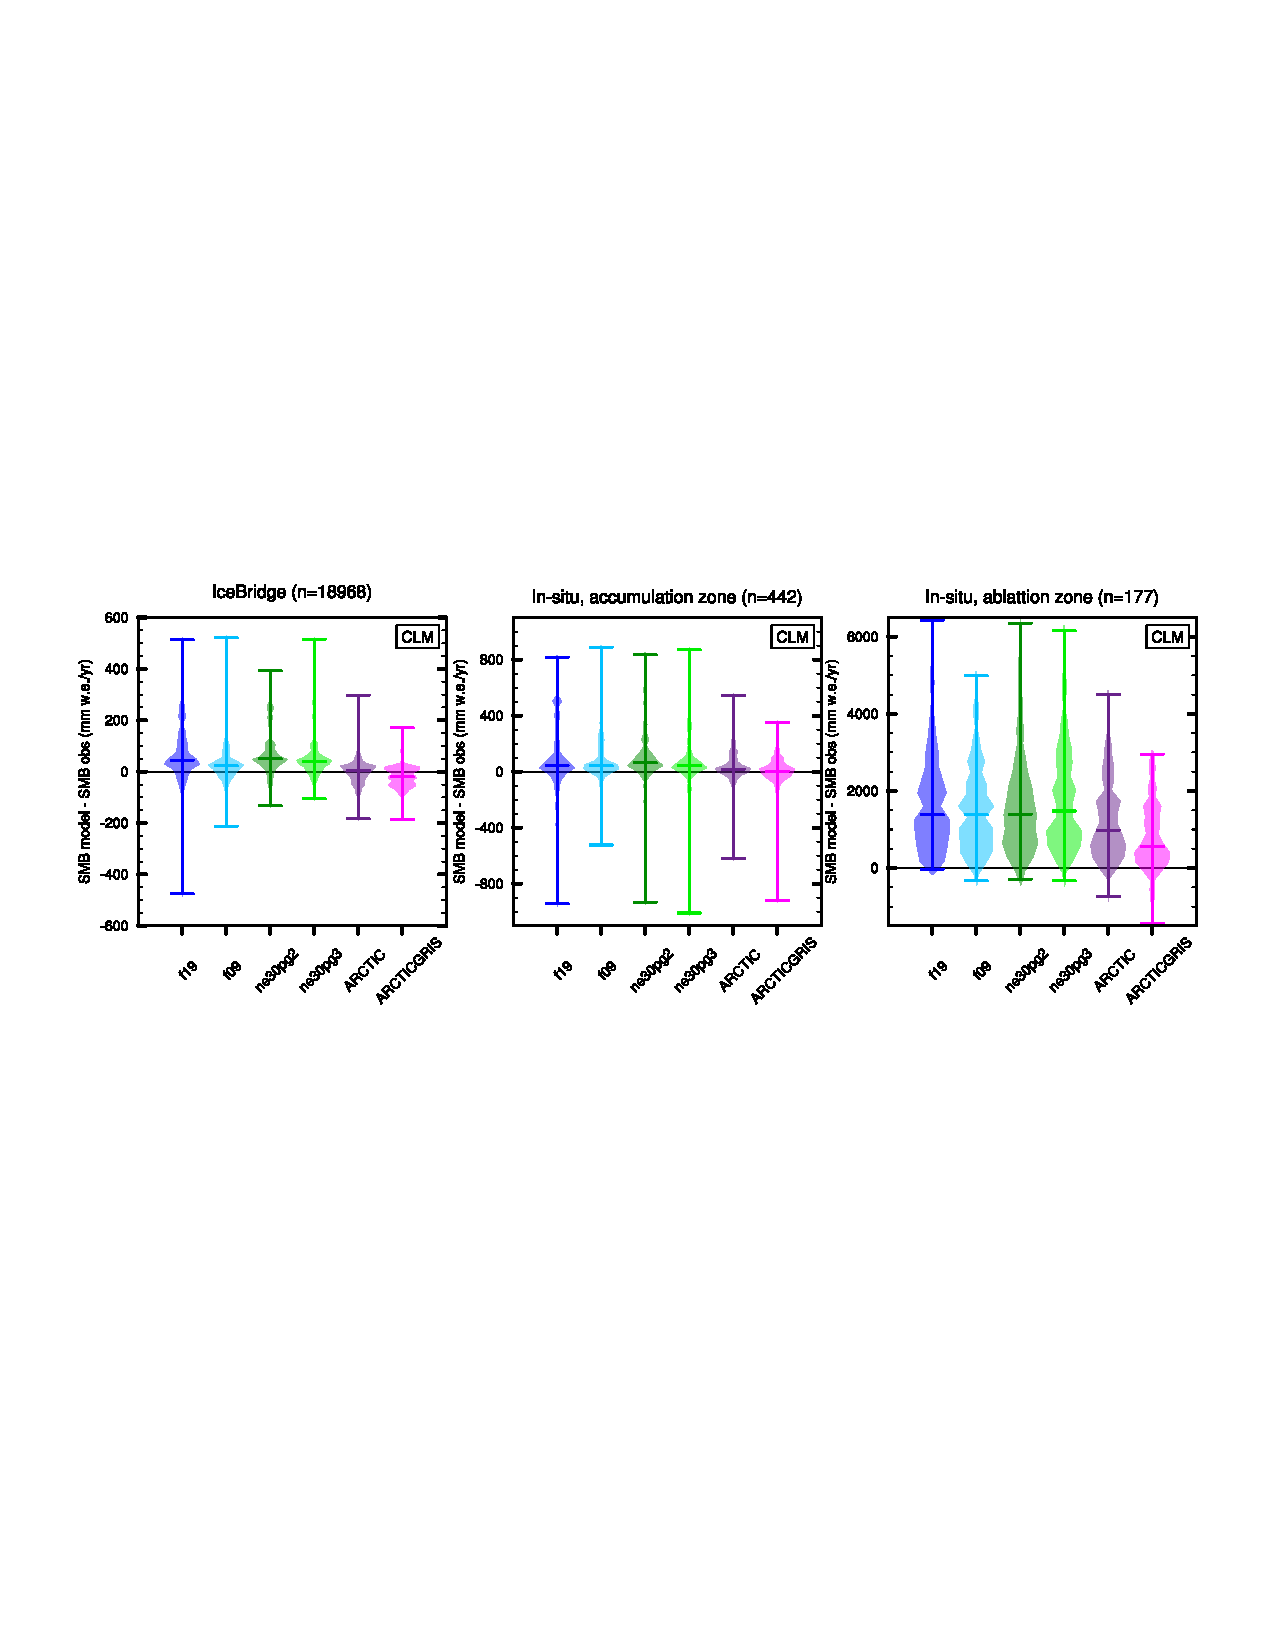
\includegraphics[width=130mm]{figs/temp_violens.pdf}
%\end{center}
%\caption{.}
%\label{fig:pointdiff}
%\end{figure}

The ``k-transect" is perhaps the most well studied transect in Greenland, as it has been regularly monitored since the 1950s. The LIVVkit has compiled the k-transect observations, shown in Figure~\ref{fig:trans} as elevation vs. SMB along the transect, with the model's simulated transects shown as well. The in-situ observation points are nicely replicated by the $ARCTCIGRIS$ run, whereas the $ARCTIC$ grid is biased positive in the higher-elevations of the ablation zone. The $f09$ grid is surprisingly competitive with the variable-resolution grids, capturing a realistic slope of the elevation-SMB curve, although it exhibits a similar positive bias as the $ARCTIC$ grid. The elevation-SMB slopes of the uniform spectral-element and $f19$ grid are too shallow, in particular at the higher elevation regions of the transect. 

Figure~\ref{fig:ztrans} shows the representation of the surface of the ice sheet along these transects in the different grids, compared to the high resolution dataset used to generate CAM topography boundary conditions. The $1^{\circ}-2^{\circ}$ grids are noticeably coarse, with only a handful of grid cells populating the transect. The $f09$ grid is a bit of an exception --since the grid cells become very narrow in the meridional direction at high latitudes, a larger number of grid cells can populate the east-west transect, consistent with its skillful representation of the ablation zone.

What the authors refer to as the ``b-transect" in northwest Greenland (Figure~\ref{fig:trans}) is characterized by orographic precipitation, resulting in the accumulation zone extending down to the ice margin. The variable resolution grids perform relatively well, with larger SMBs at lower elevations where the precipitation rates are highest, whereas the $1^{\circ}-2^{\circ}$ grids underestimate the SMB in these lower elevation regions. Only the variable resolution grids can capture the local reduction in SMB in the 1500-2000 m region. The skill of the variable-resolution grids is clearly related to the more accurate representation of the steepness of the transect, while also capturing the protrusion around 1500-2000 m that coincides with the local minimum in SMB (Figure~\ref{fig:ztrans}).

%\begin{figure}[t]
%\begin{center}
%         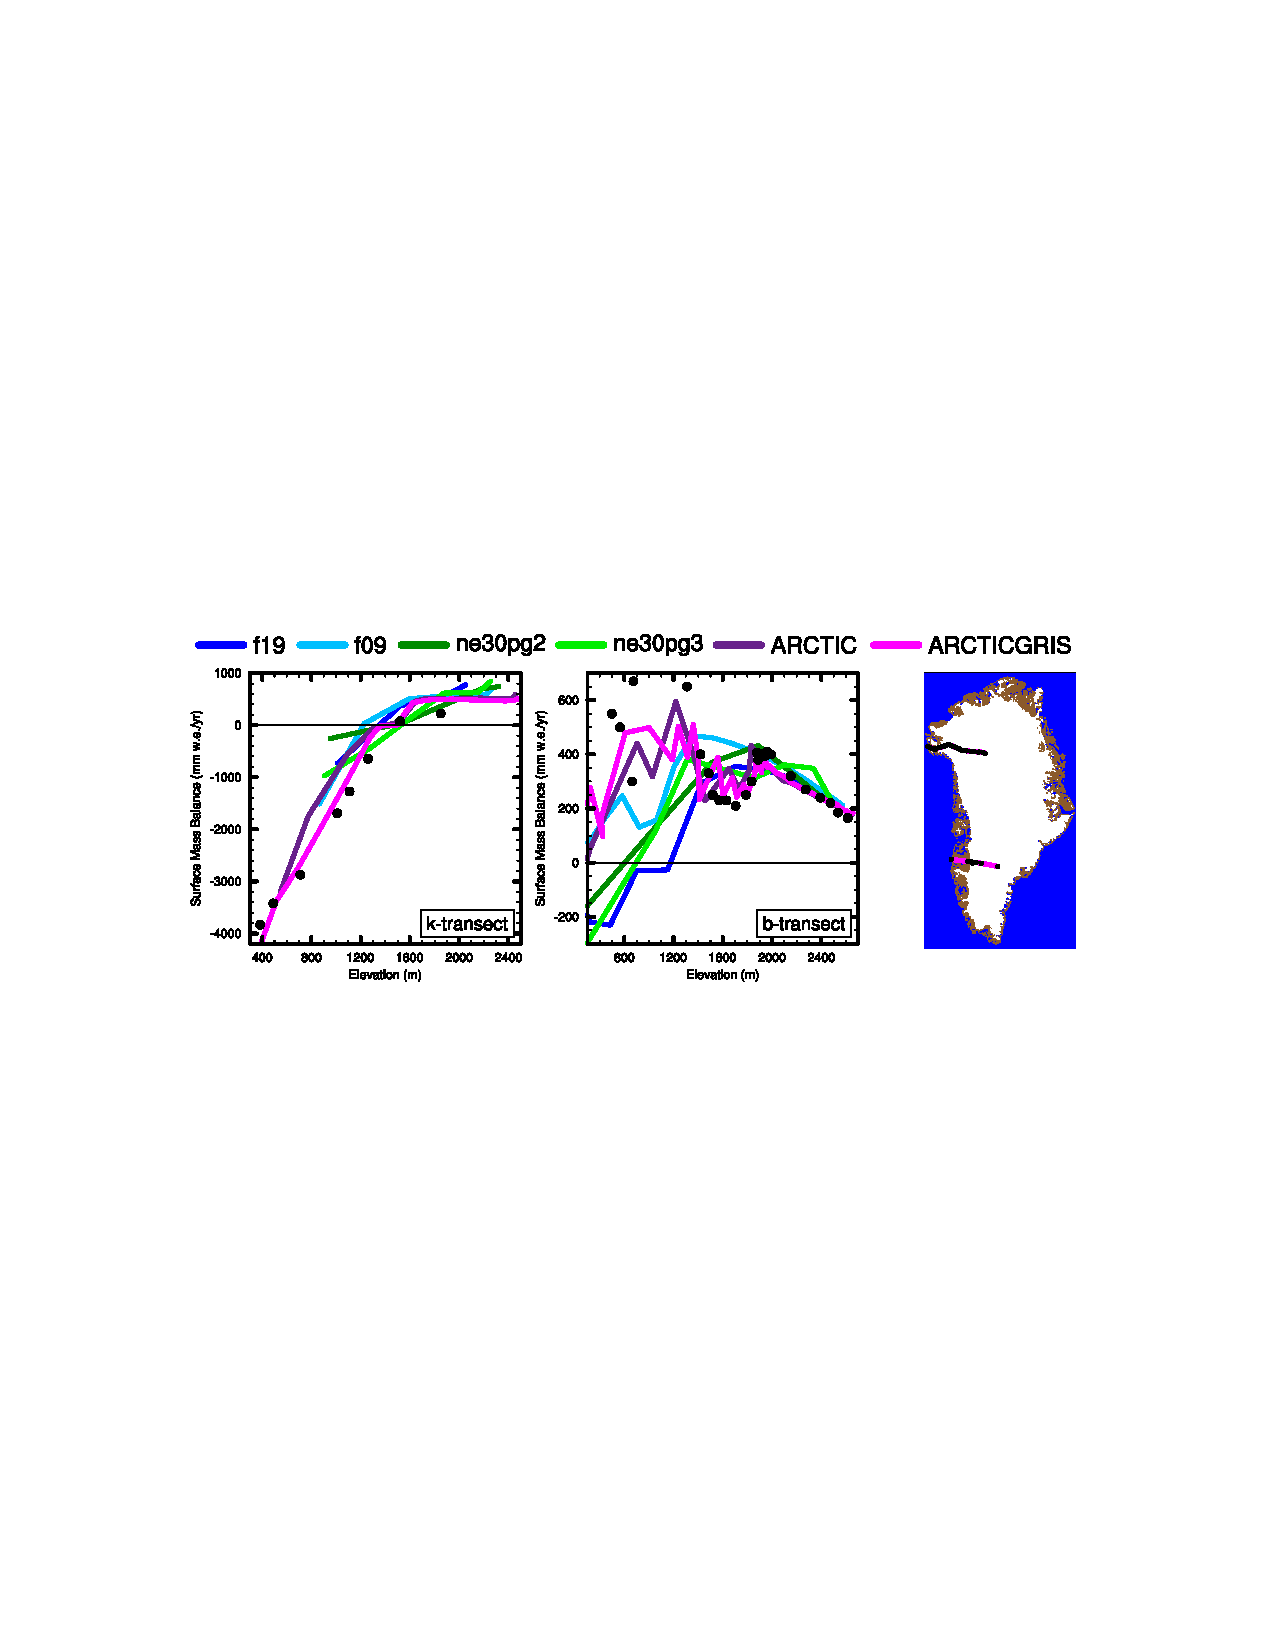
\includegraphics[width=130mm]{figs/temp_transect_obsperiod.pdf}
%\end{center}
%\caption{.}
%\label{fig:trans}
%\end{figure}

\begin{figure}[t]
\begin{center}
\begin{tabular}{cccc}
         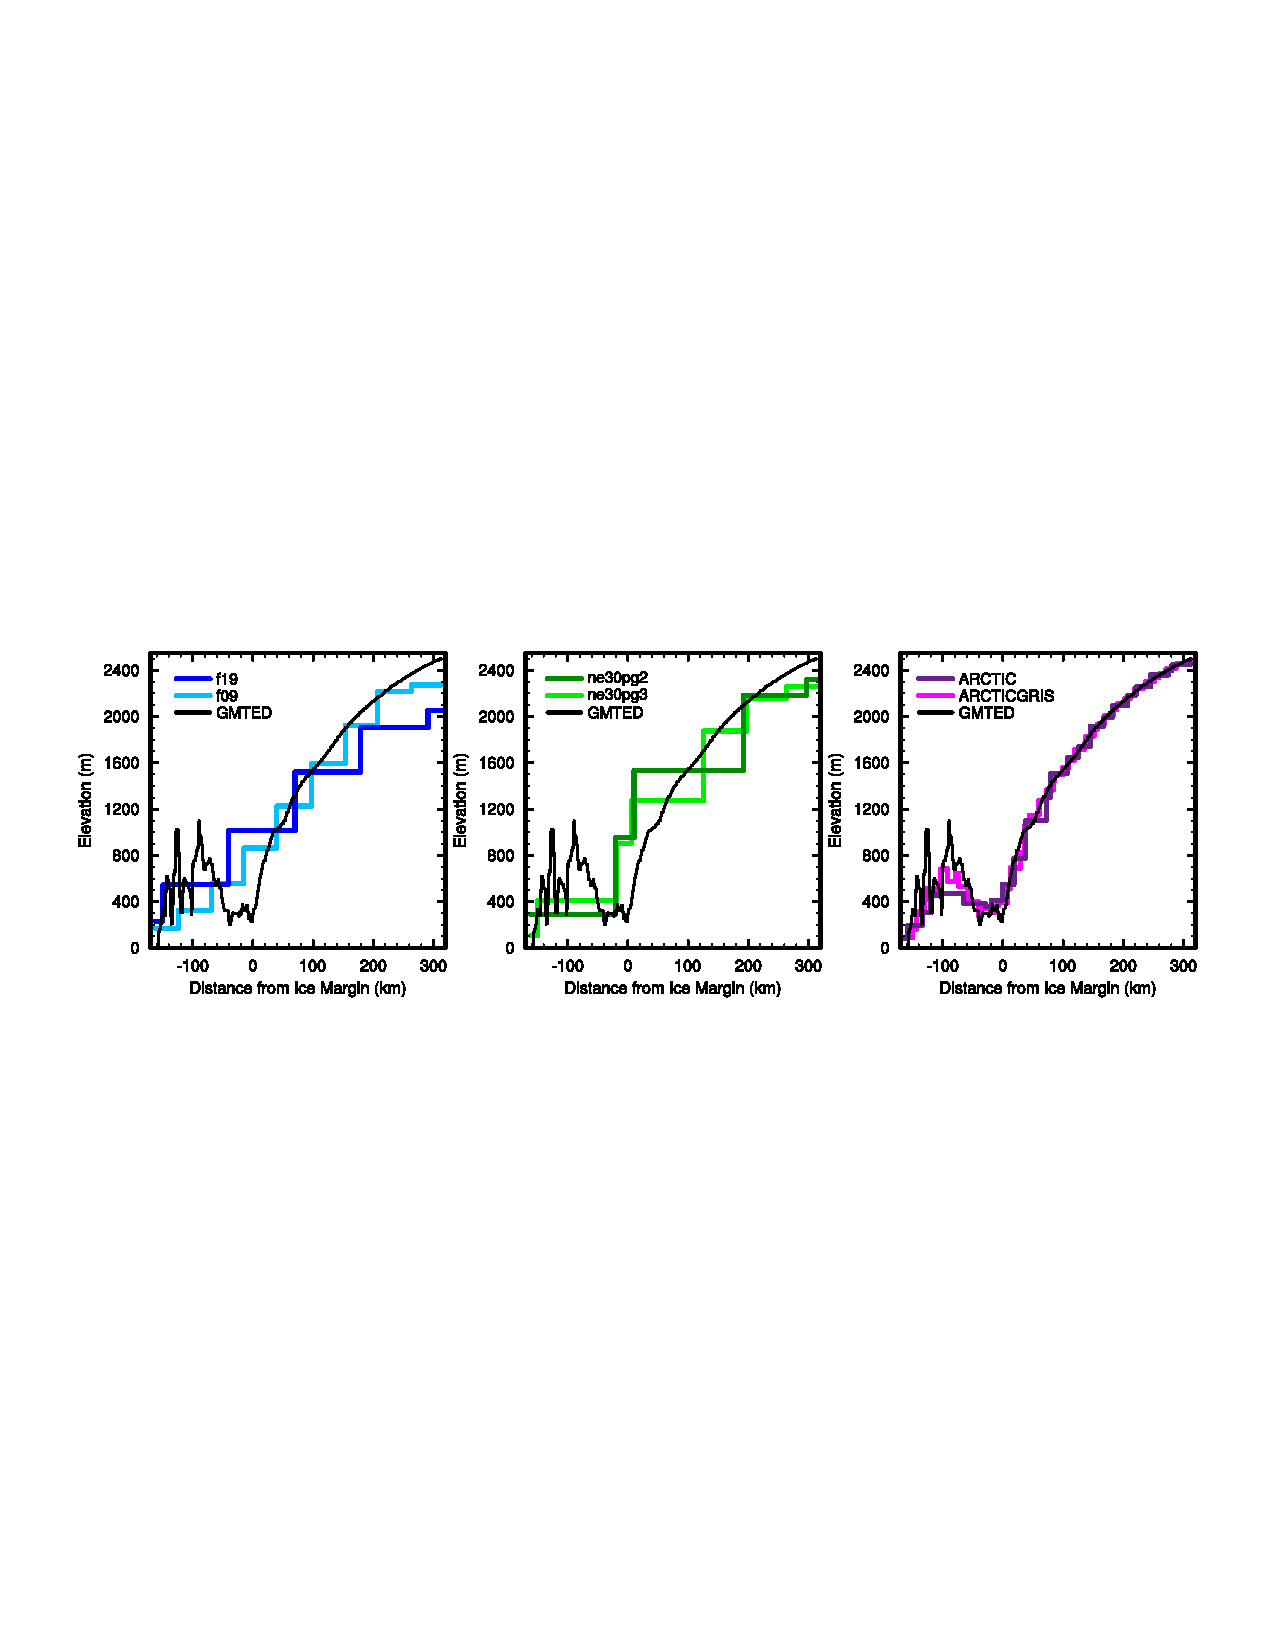
\includegraphics[width=130mm]{figs/temp_ktransect.pdf} \\
         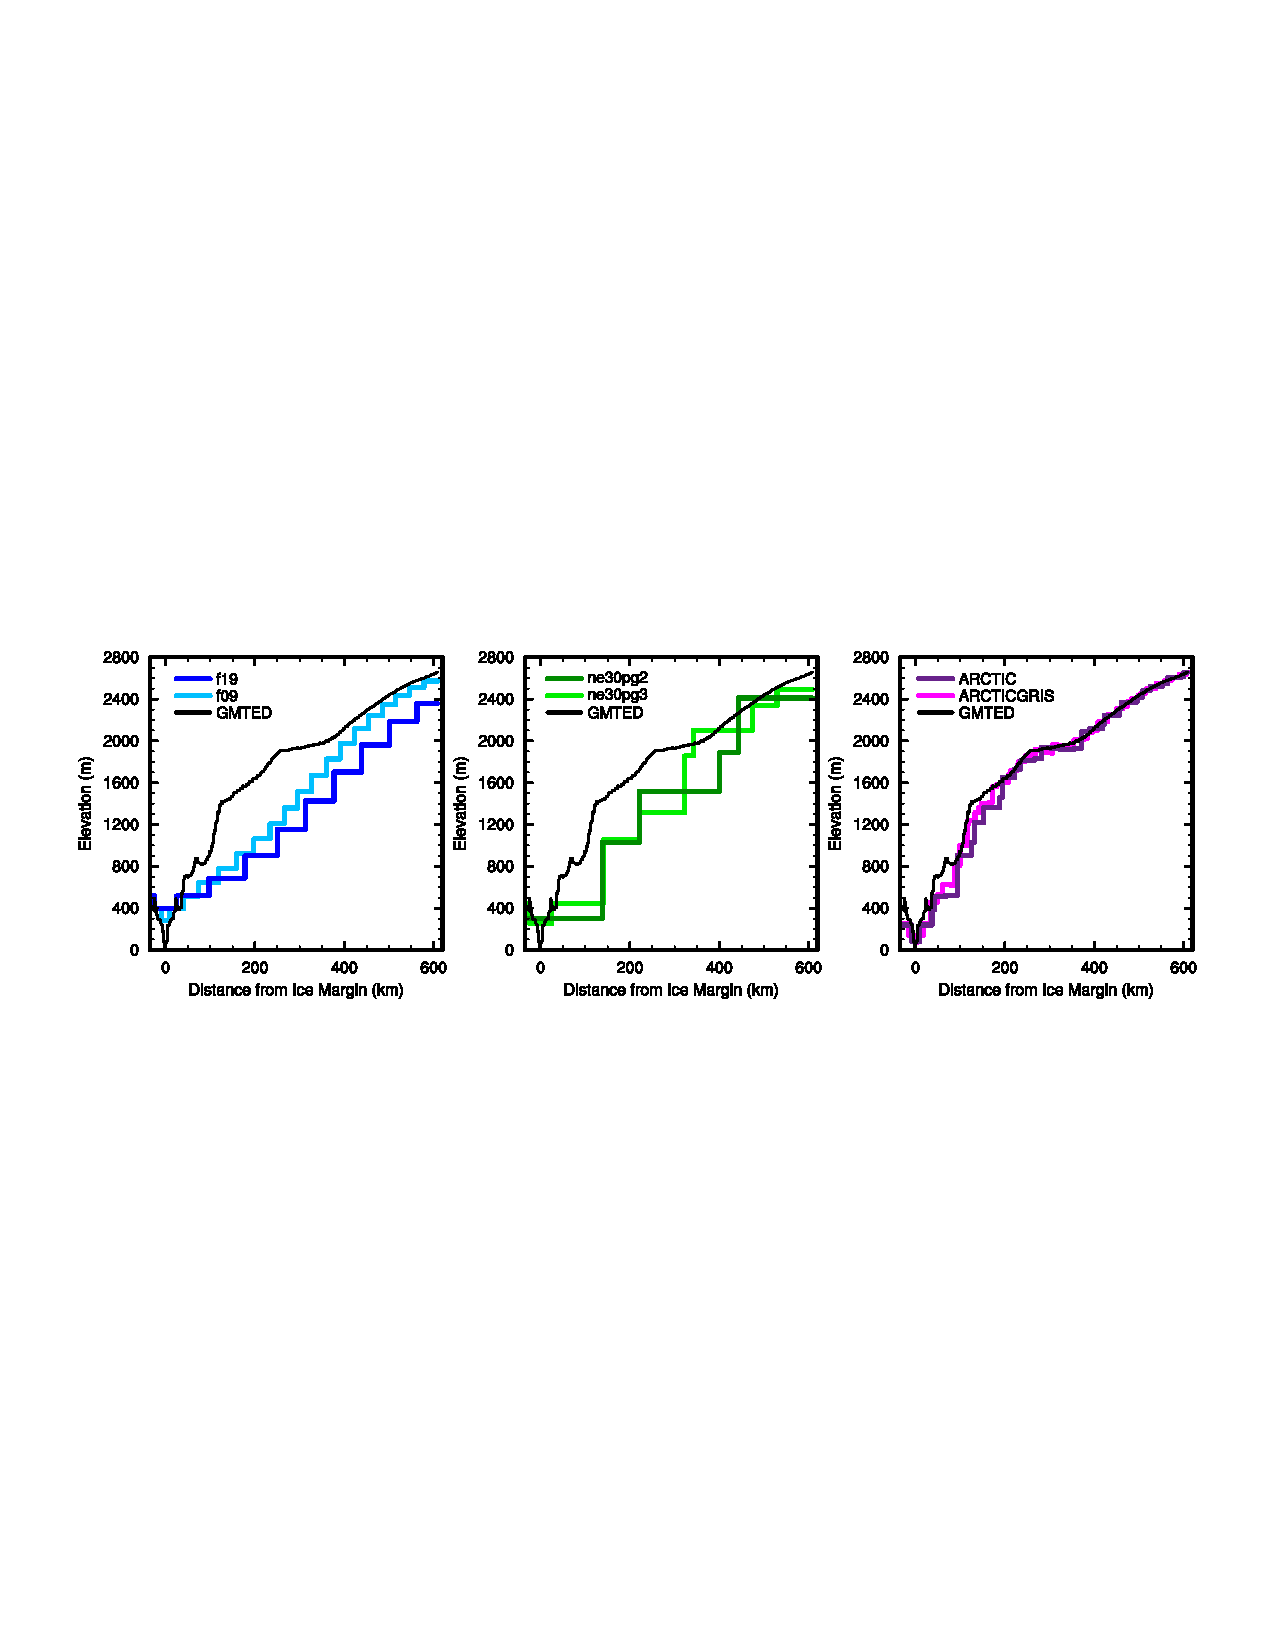
\includegraphics[width=130mm]{figs/temp_btransect.pdf} \\
\end{tabular}
\end{center}
\caption{.}
\label{fig:ztrans}
\end{figure}

To give an idea of what the ablation zones look like in the highest resolution $ARCTCIGRIS$ grid, Figure~\ref{fig:viz} is a still from a visualization produced by the authors. It shows the daily mean surface mass balance during the height of the melt season in year 1981 of the simulation. The ablation zone appears to be well resolved in the $ARCTICGRIS$ grid. The full visualization is publicly available on youtube.com\footnote{\url{https://www.youtube.com/watch?v=YwHgqDu75s8&t=4s&ab_channel=NCARVisLab}}.

\begin{figure}[t]
\begin{center}
         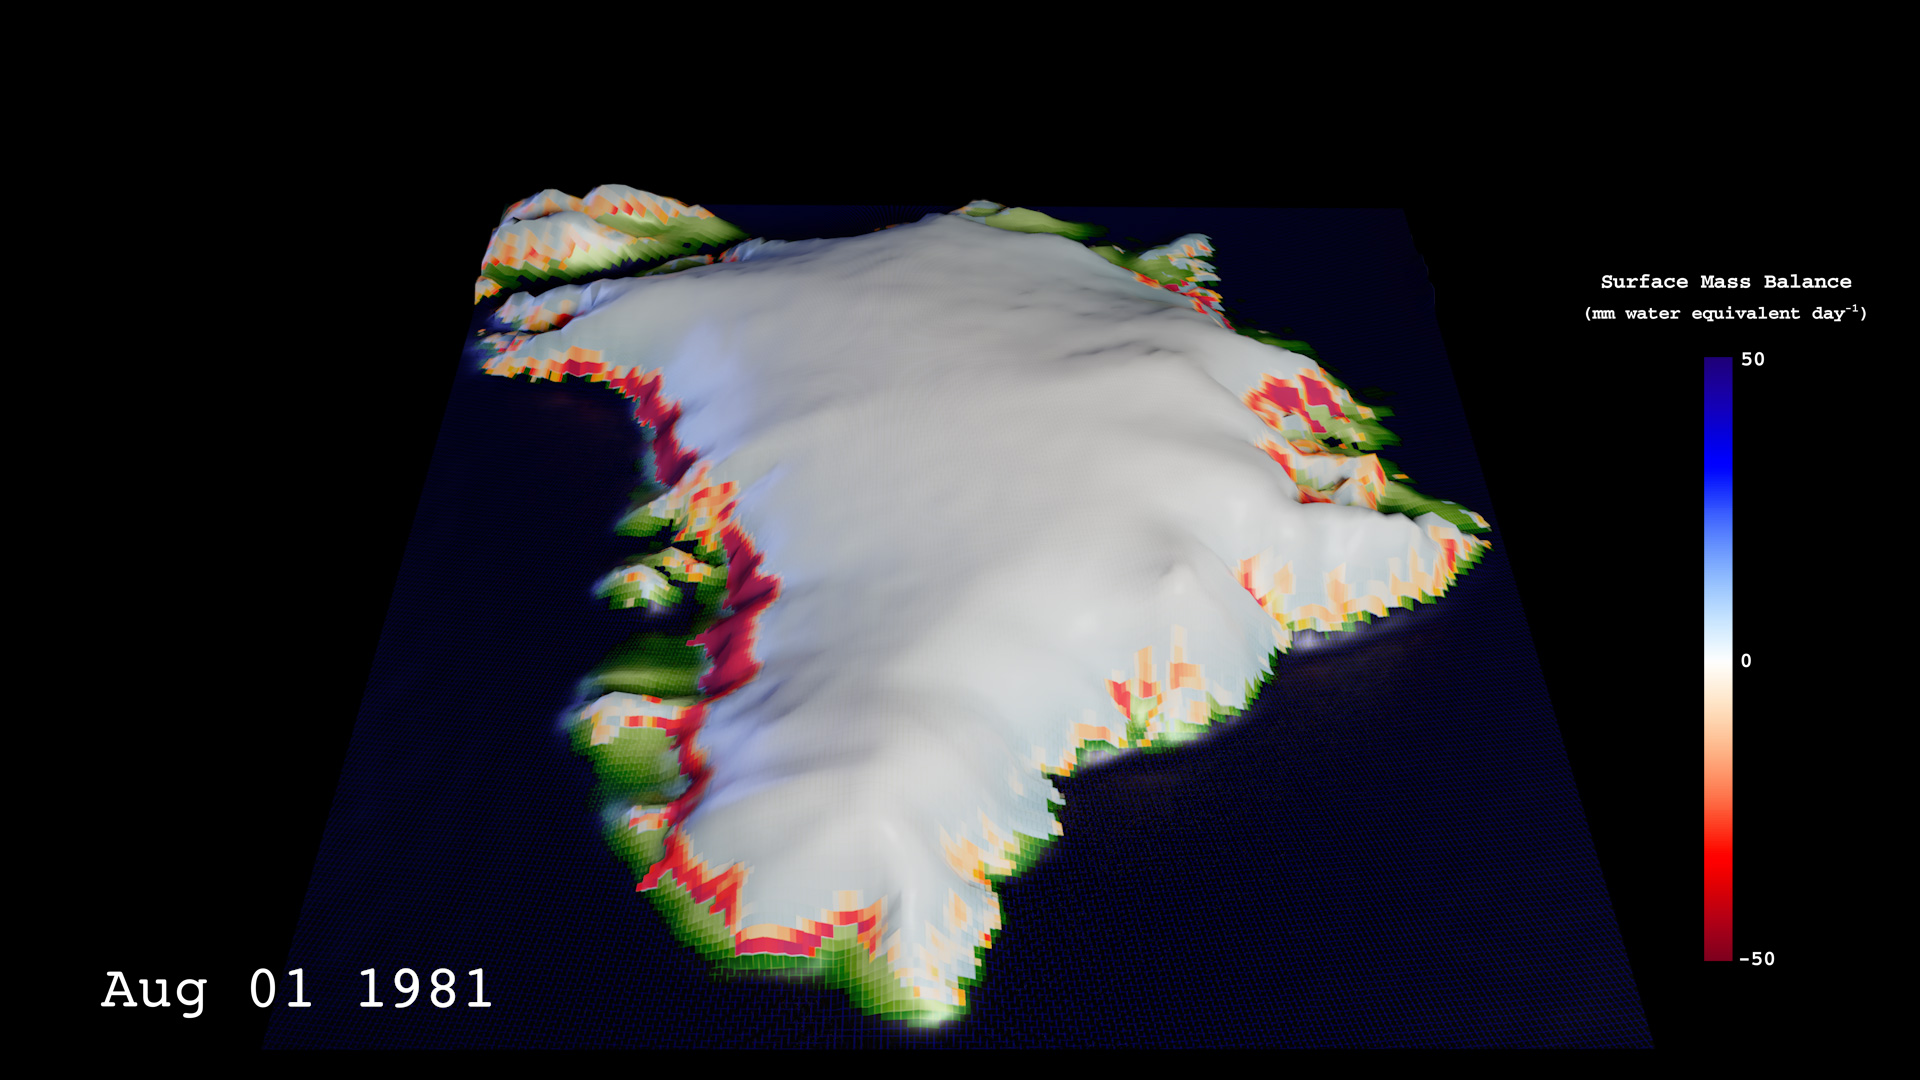
\includegraphics[width=130mm]{figs/Vis1923.jpg}
\end{center}
\caption{.}
\label{fig:viz}
\end{figure}

\subsection{Precipitation extremes}

Synoptic storms are tracked and analyzed using TempestExtremes \cite{UETAL2021}. As the $ARCTIC$ grid contains $\frac{1}{4}^{\circ}$ refinement north of about $45^{\circ}$ latitude, the storm tracker is applied to this region for the $ARCTIC$ and $ne30pg3$ run to identify differences in storm characteristics due to horizontal resolution. Figure~\ref{fig:comp-mean} shows the mean precipitation rates averaged over all January storms identified by TempestExtremes. The iconic comma structure of the synoptic cyclones is simulated in $ne30pg3$ and $ARCTIC$ grids, with the magnitudes about the same in these two grids, with perhaps a marginal increase in precipitation rates in the storm center of the $ARCTIC$ grid. For good measure, the $ne30pg3^{*}$ run is also plotted, and looks more-or-less identical to the $ne30pg3$ run.

As has been previously reported, horizontal resolution can have large impacts on extreme precipitation events. Figure~\ref{fig:comp-pdf} is a PDF of the precipitation rates associated with synoptic storms, by month. The PDFs are constructed by sampling all the precipitation rates within $30^{\circ}$ of the storm center, for each point on the storm track and for all storms. The PDFs are evaluated on an identical composite grid for all runs, and so storm statistics are not impacted by differences in output resolution. The $ARCTIC$ run has larger extreme precipitation rates compared to $ne30pg3$ in every month, but the increase is greatest in the summer months, which coincides with the most extreme events of the year. This is primarily due to an increase in resolution, and not the reduced physics times-step; the $ne30pg3^{*}$ only marginally increases the precipitation rates compared with $ne30pg3$.

The extreme precipitation rates in the $ARCTIC$ run are closer to the ERA5 reanalysis than in $ne30pg3$ (Figure~\ref{fig:comp-pdf}). It's difficult to know the extent that the extreme precipitation rates in ERA5 are constrained by data assimilation, or whether these precipitation rates are due to using a similar $\frac{1}{4}^{\circ}$ model as the $ARCTIC$ grid. However, it is well documented that $\frac{1}{4}^{\circ}$ models are more skillful at simulating extreme events \cite{BetAl2013JC,OETAL2016JAMES}, and so this is an additional benefit of the variable-resolution grids.

%\begin{figure}[t]
%\begin{center}
%         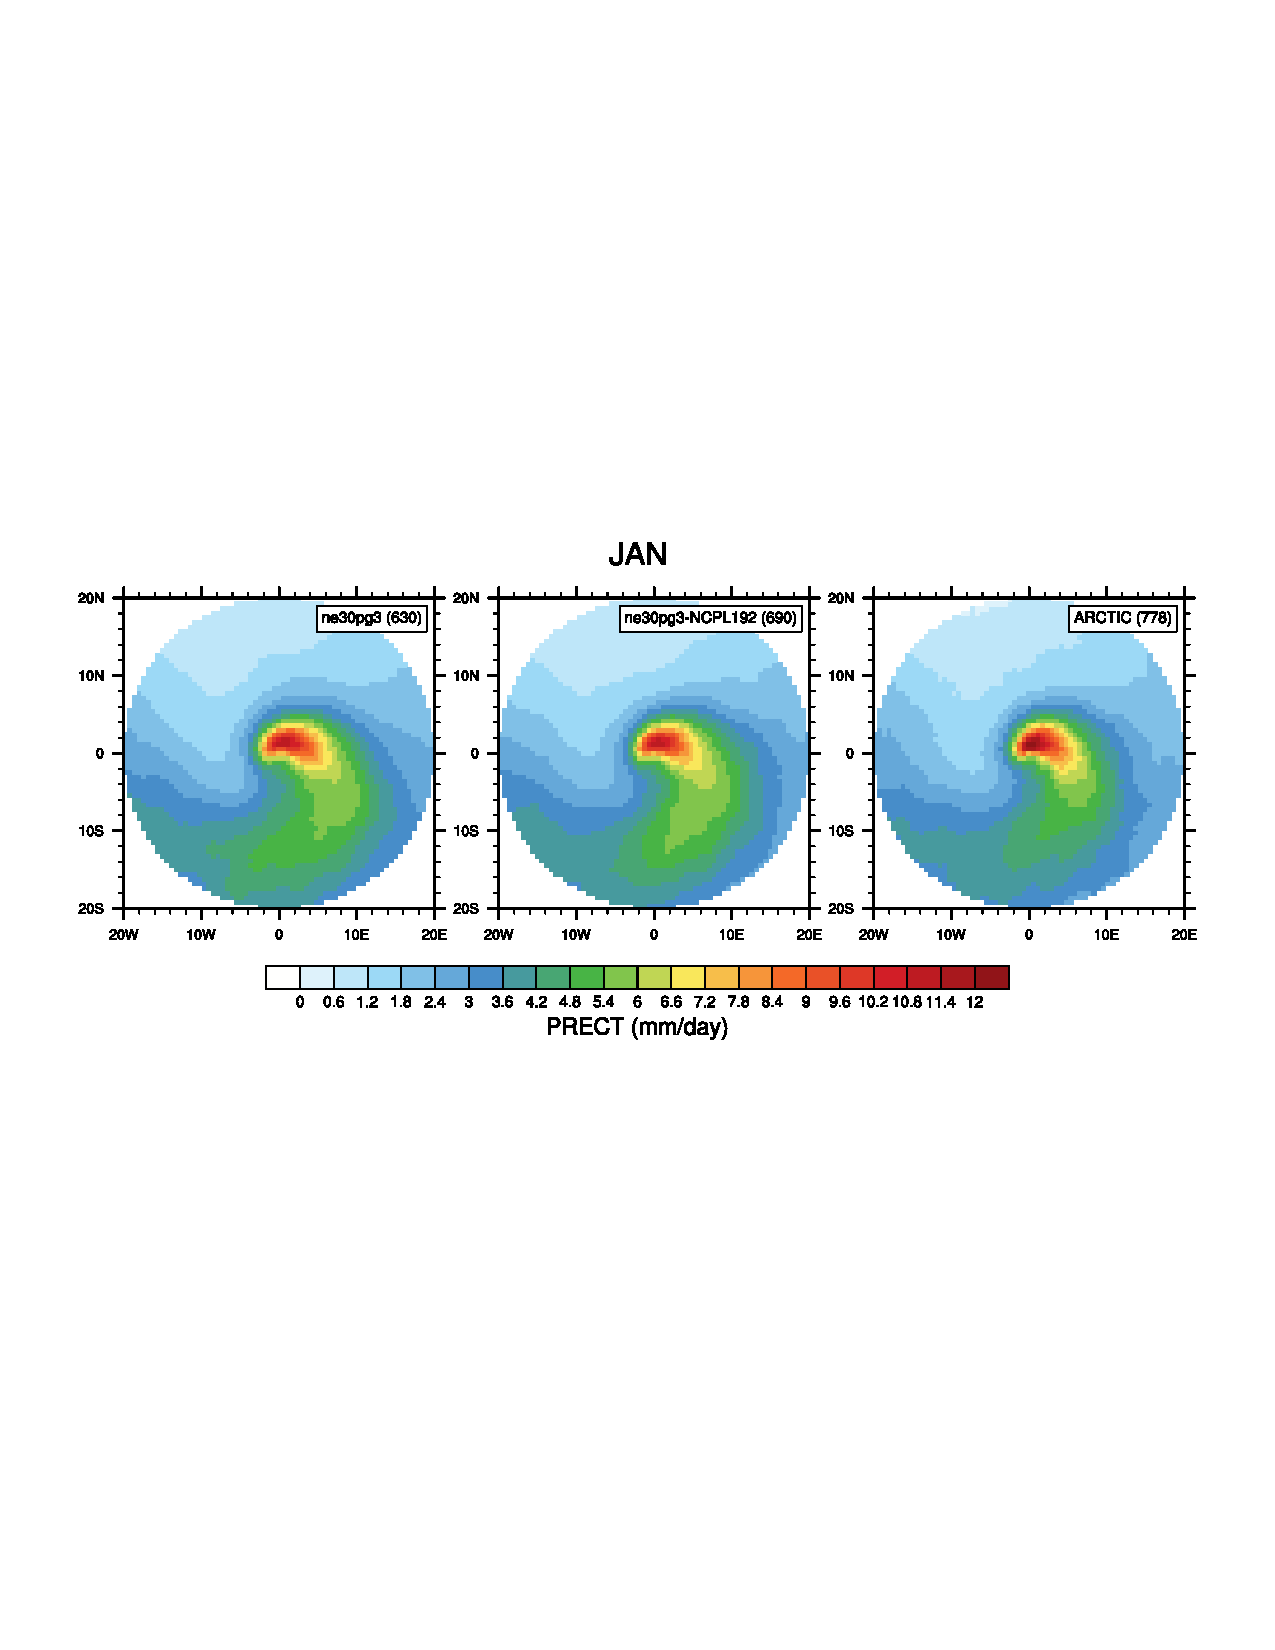
\includegraphics[width=130mm]{figs/temp_composite_ge45N_JAN-PRECT.pdf}
%\end{center}
%\caption{.}
%\label{fig:comp-mean}
%\end{figure}

\begin{figure}[t]
\begin{center}
         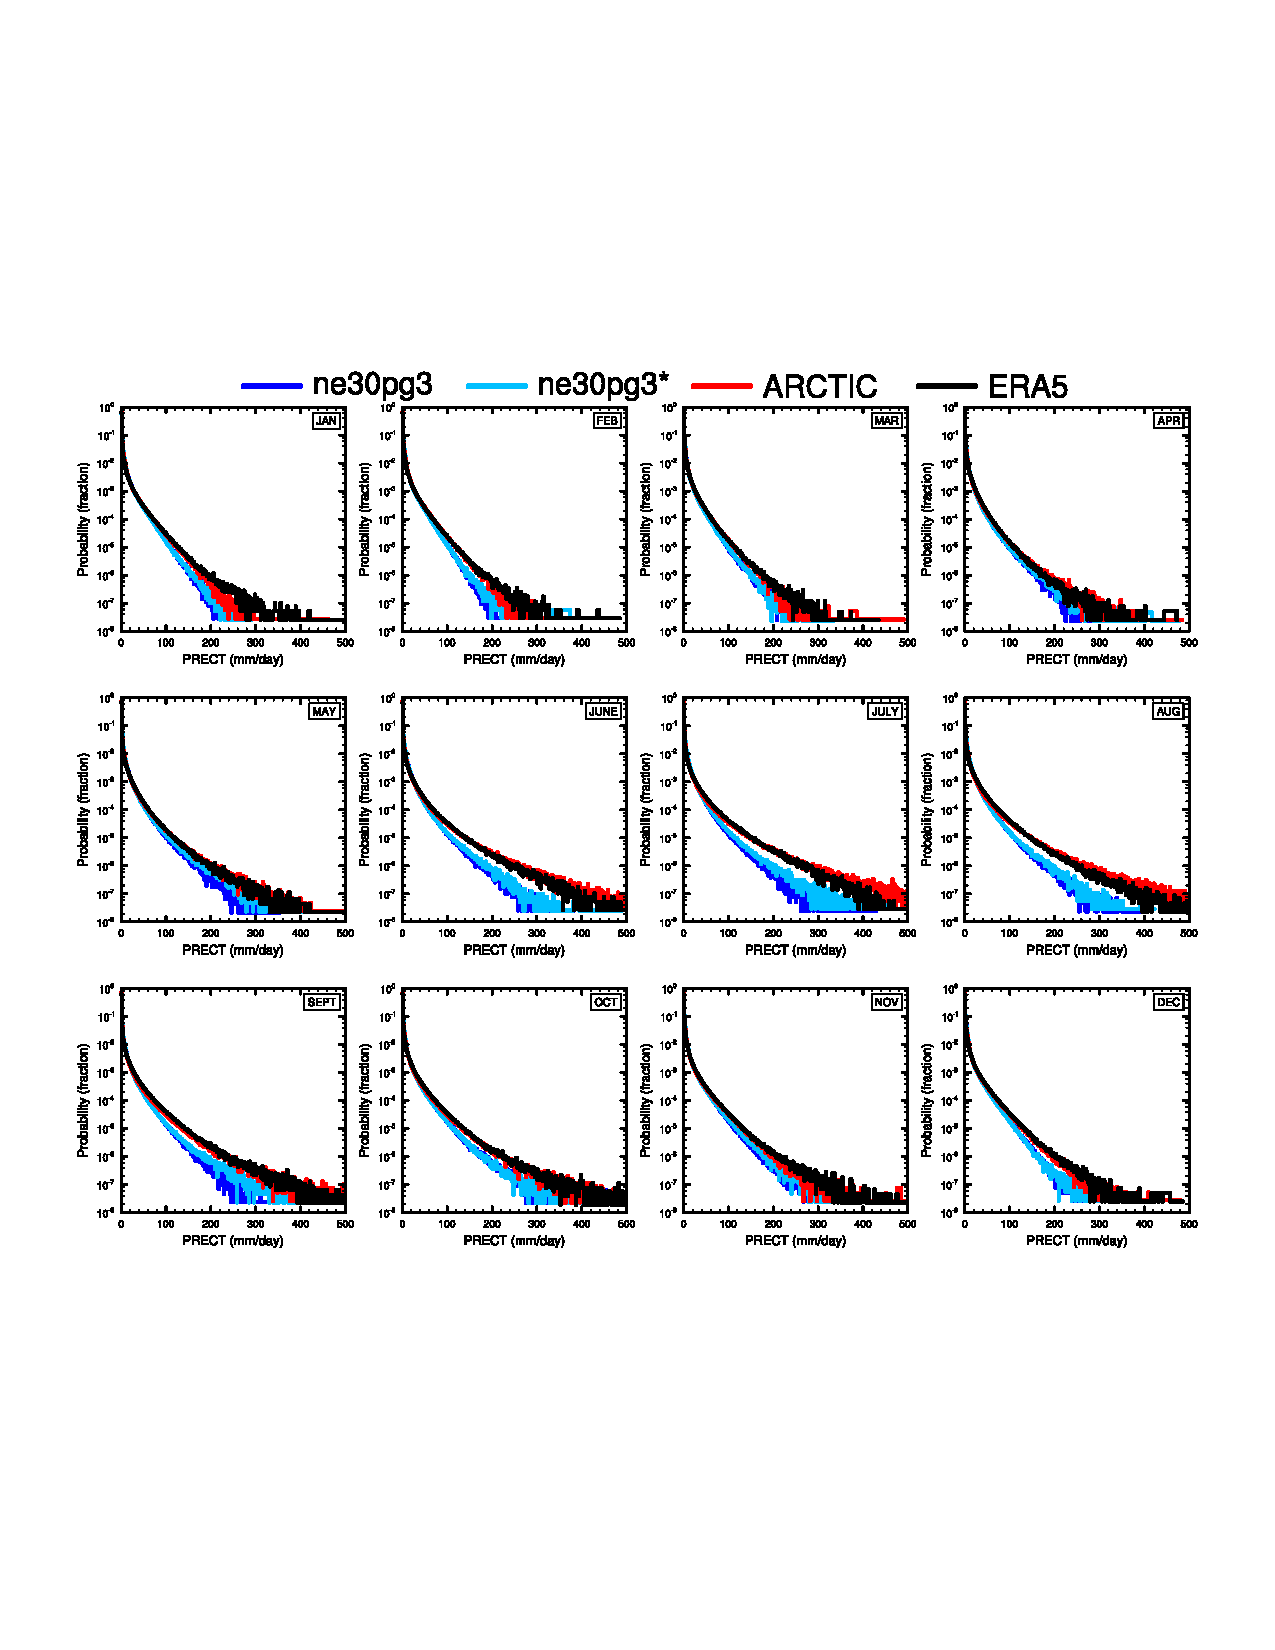
\includegraphics[width=130mm]{figs/temp_composite_ge45N_pdf.pdf}
\end{center}
\caption{.}
\label{fig:comp-pdf}
\end{figure}

\section{Conclusions}\label{sec:conclusions}

Six grids from different dynamical cores in CESM2.2 are evaluated in an AMIP-style configuration for their performance over the Arctic and in simulating the Greenland Ice Sheet (GrIS) surface mass balance (SMB). The $1-2^{\circ}$ finite-volume grids have enhanced resolution over Polar regions due to the convergence of meridian lines, although a polar filter is employed to prevent features from forming at this higher resolution. Spectral-element grids comparable to the resolution of the finite-volume grids have an isotropic grid structure, meaning the grid resolution is similar over the entire domain. Two variable-resolution grids were developed and introduced into CESM2.2 as part of this work. They use the spectral-element dycore; the $ARCTIC$ grid has $\frac{1}{4}^{\circ}$ refinement over the broader Arctic, whereas the $ARCTICGRIS$ grid is identical except it has an $\frac{1}{8}^{\circ}$ patch of refinement over Greenland.

In general, the finite-volume grids have colder summer temperatures over the Arctic, and the spectral-element grids (incl. the variable-resolution grids) are warmer. The cloud biases in all the uniform resolution grids, whether finite-volume or spectral-elements, are similar, in general being too cloudy over Arctic land masses. The variable-resolution grids largely improve the cloud biases. It should be emphasized that our analysis is specific to the Arctic summer due to its relevance to melt rates over GrIS; improved clouds in the Arctic should not be taken to mean that lower latitude regions have an improved cloud field as well.

At the regional level, a halo of negative cloud bias is found around the oceanic perimeter of Greenland in all $1-2^{\circ}$ grids, and is absent in the variable-resolution grids. This halo bias coincides with a positive cloud bias over the interior of the ice sheet. This has been traced back to the inadequacy of the lower resolution grids to resolve the orographic precipitation process in Greenland. Synoptic systems moving into Greenland are not sufficiently lifted when encountering the steep ice margins due to overly smooth topography in the $1-2^{\circ}$ grids. As as result, moisture penetrates accross the ice margin and dumps excess precipitation into the interior of the GrIS, instead of being concentrated closer to the coastal margins as indicated by observations. This results in a positive precipitation and cloud bias in the ice sheet interior, and a halo of low cloud bias about the perimeter of Greenland. The agreement of different observational data products on this bias lends confidence  in attributing the cause of the precipitation and cloud biases. The variable-resolution grids compare more favorably to the observations and indicate the orographic precipitation process in Greenland is largely resolved.

The primary source and sink terms of the SMB equation are integrated over the GrIS, and evaluated in the six grids. The uniform $1-2^{\circ}$ grids all have large positive accumulation biases owing to their inability to resolve the orographic precipitation process. The uniform spectral-element grids have larger accumulation biases, suggesting that the finite-volume grids are more skillful at resolving the precipitation processes due to their finer grid spacing over Greenland, despite the polar filter. The variable resolution grids have the most accurate accumulation rates of all the grids. 

The primary mass sink term of the GrIS, ice/snow melt, expresses similar biases as the accumulation rates. The uniform resolution spectral-element grids melt too much, while the finite-volume grids have reduced biases. It's more difficult to attribute these biases to grid resolution alone; the finite-volume grids have colder summers that is consistent with their lower melt bias. However, the $ARCTICGRIS$ grid has the warmest summer temperatures of all grids, yet it has reduced melting compared to the uniform resolution spectral-element grids. This suggests that grid resolution is responsible for a large fraction of the melt biases. That the melt process would be sensitive to grid resolution is intuitive, since local elevation impacts on temperature and melting is largely handled by the land model, which does not have a pole problem because there is no horizontal dynamics. The larger number of grid cells in the ablation zone in the finite-volume grids seems to more accurately resolve the melt process relative to the uniform resolution spectral-element grids, in which the ablation zone is made up of substantially fewer grid cells.



% \section{Materials and Methods}
% Here is text on Materials and Methods.
%
% \subsection{A descriptive heading about methods}
% More about Methods.
%
% \section{Data} (Or section title might be a descriptive heading about data)
%
% \section{Results} (Or section title might be a descriptive heading about the
% results)
%

%\begin{figure}[t]
%\begin{center}
%         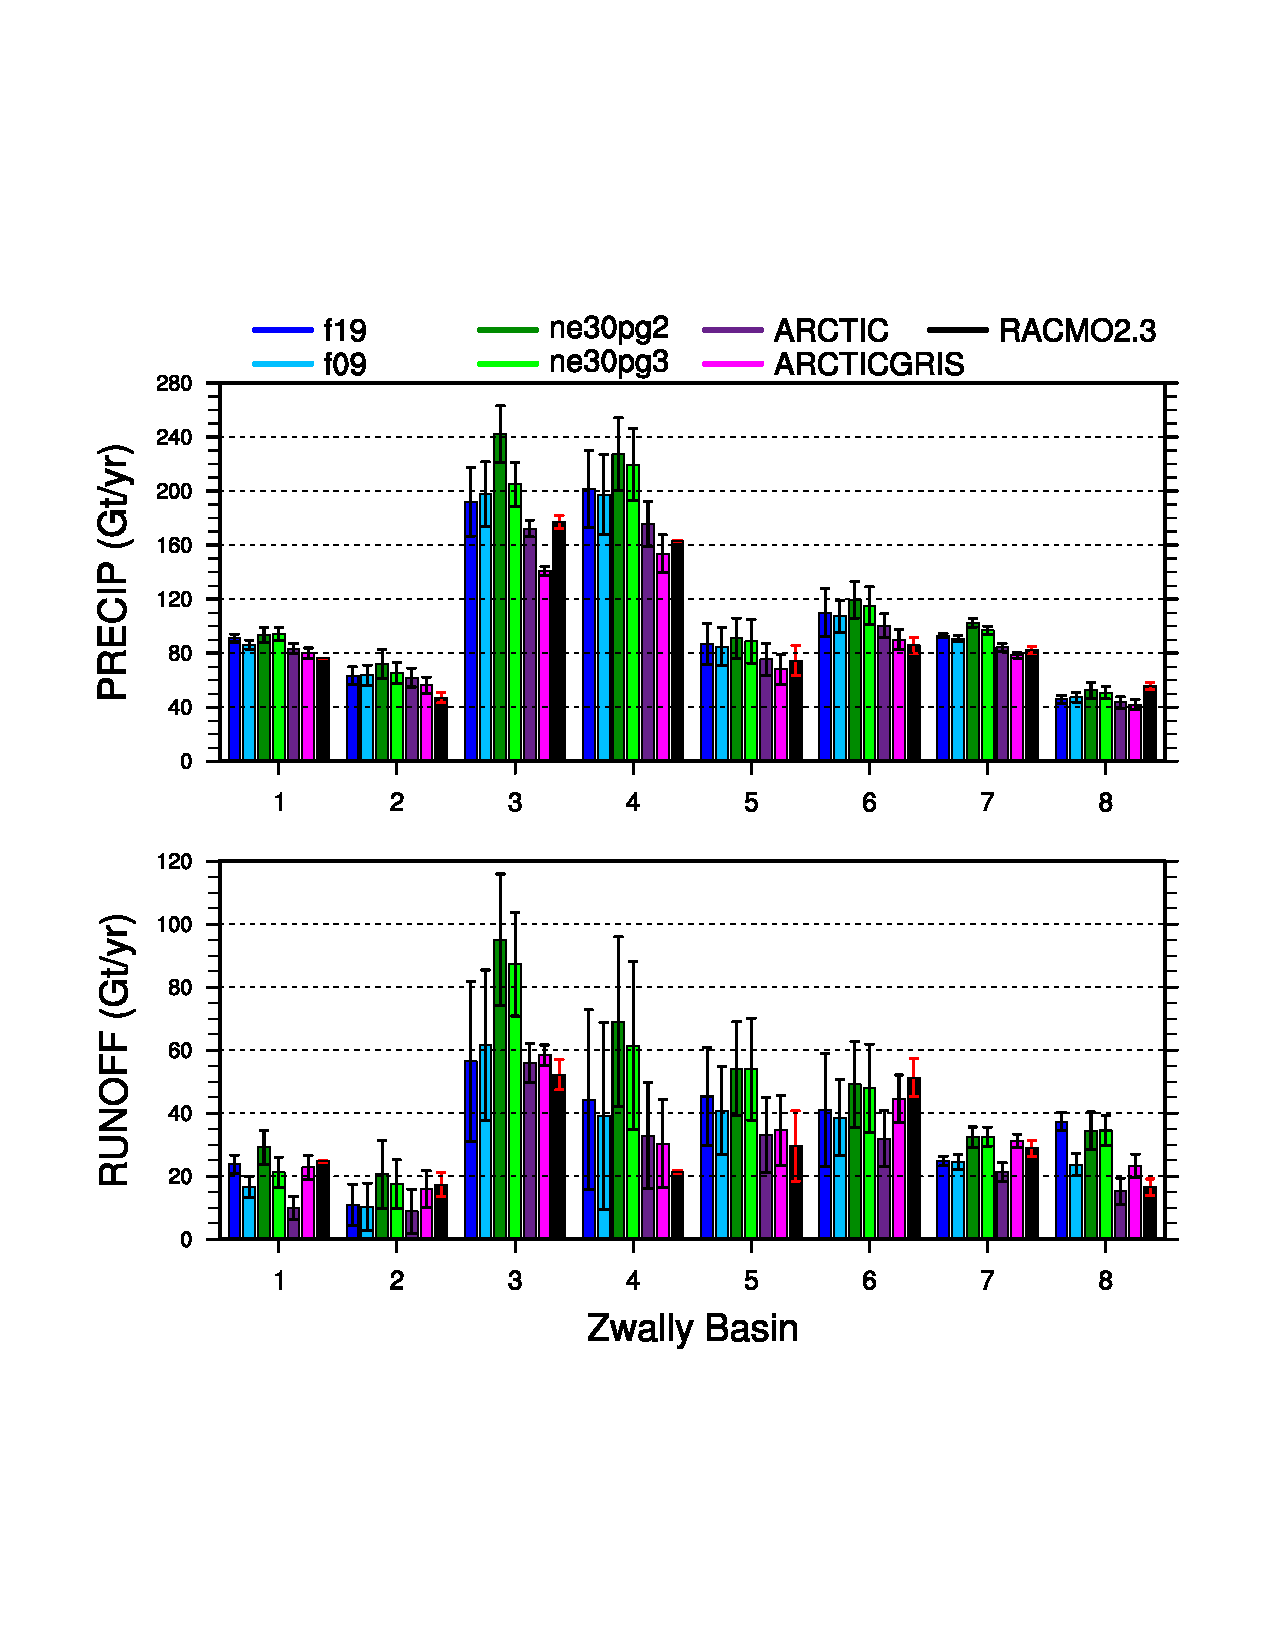
\includegraphics[width=100mm]{figs/temp_tseries_BASIN_uqmap.pdf}
%\end{center}
%\caption{.}
%\label{fig:zwally}
%\end{figure}

%Text here ===>>>


%%

%  Numbered lines in equations:
%  To add line numbers to lines in equations,
%  \begin{linenomath*}
%  \begin{equation}
%  \end{equation}
%  \end{linenomath*}



%% Enter Figures and Tables near as possible to where they are first mentioned:
%
% DO NOT USE \psfrag or \subfigure commands.
%
% Figure captions go below the figure.
% Table titles go above tables;  other caption information
%  should be placed in last line of the table, using
% \multicolumn2l{$^a$ This is a table note.}
%
%----------------
% EXAMPLE FIGURES
%
% \begin{figure}
% \includegraphics{example.png}
% \caption{caption}
% \end{figure}
%
% Giving latex a width will help it to scale the figure properly. A simple trick is to use \textwidth. Try this if large figures run off the side of the page.
% \begin{figure}
% \noindent\includegraphics[width=\textwidth]{anothersample.png}
%\caption{caption}
%\label{pngfiguresample}
%\end{figure}
%
%
% If you get an error about an unknown bounding box, try specifying the width and height of the figure with the natwidth and natheight options. This is common when trying to add a PDF figure without pdflatex.
% \begin{figure}
% \noindent\includegraphics[natwidth=800px,natheight=600px]{samplefigure.pdf}
%\caption{caption}
%\label{pdffiguresample}
%\end{figure}
%
%
% PDFLatex does not seem to be able to process EPS figures. You may want to try the epstopdf package.
%

%
% ---------------
% EXAMPLE TABLE
%
% \begin{table}
% \caption{Time of the Transition Between Phase 1 and Phase 2$^{a}$}
% \centering
% \begin{tabular}{l c}
% \hline
%  Run  & Time (min)  \\
% \hline
%   $l1$  & 260   \\
%   $l2$  & 300   \\
%   $l3$  & 340   \\
%   $h1$  & 270   \\
%   $h2$  & 250   \\
%   $h3$  & 380   \\
%   $r1$  & 370   \\
%   $r2$  & 390   \\
% \hline
% \multicolumn{2}{l}{$^{a}$Footnote text here.}
% \end{tabular}
% \end{table}

%% SIDEWAYS FIGURE and TABLE
% AGU prefers the use of {sidewaystable} over {landscapetable} as it causes fewer problems.
%
% \begin{sidewaysfigure}
% \includegraphics[width=20pc]{figsamp}
% \caption{caption here}
% \label{newfig}
% \end{sidewaysfigure}
%
%  \begin{sidewaystable}
%  \caption{Caption here}
% \label{tab:signif_gap_clos}
%  \begin{tabular}{ccc}
% one&two&three\\
% four&five&six
%  \end{tabular}
%  \end{sidewaystable}

%% If using numbered lines, please surround equations with \begin{linenomath*}...\end{linenomath*}
%\begin{linenomath*}
%\begin{equation}
%y|{f} \sim g(m, \sigma),
%\end{equation}
%\end{linenomath*}

%%% End of body of article

%%%%%%%%%%%%%%%%%%%%%%%%%%%%%%%%
%% Optional Appendix goes here
%
% The \appendix command resets counters and redefines section heads
%
% After typing \appendix
%
%\section{Here Is Appendix Title}
% will show
% A: Here Is Appendix Title
%
%\appendix
%\section{Here is a sample appendix}

%%%%%%%%%%%%%%%%%%%%%%%%%%%%%%%%%%%%%%%%%%%%%%%%%%%%%%%%%%%%%%%%
%
% Optional Glossary, Notation or Acronym section goes here:
%
%%%%%%%%%%%%%%
% Glossary is only allowed in Reviews of Geophysics
%  \begin{glossary}
%  \term{Term}
%   Term Definition here
%  \term{Term}
%   Term Definition here
%  \term{Term}
%   Term Definition here
%  \end{glossary}

%
%%%%%%%%%%%%%%
% Acronyms
%   \begin{acronyms}
%   \acro{Acronym}
%   Definition here
%   \acro{EMOS}
%   Ensemble model output statistics
%   \acro{ECMWF}
%   Centre for Medium-Range Weather Forecasts
%   \end{acronyms}

%
%%%%%%%%%%%%%%
% Notation
%   \begin{notation}
%   \notation{$a+b$} Notation Definition here
%   \notation{$e=mc^2$}
%   Equation in German-born physicist Albert Einstein's theory of special
%  relativity that showed that the increased relativistic mass ($m$) of a
%  body comes from the energy of motion of the body—that is, its kinetic
%  energy ($E$)—divided by the speed of light squared ($c^2$).
%   \end{notation}




%%%%%%%%%%%%%%%%%%%%%%%%%%%%%%%%%%%%%%%%%%%%%%%%%%%%%%%%%%%%%%%%
%
%  ACKNOWLEDGMENTS
%
% The acknowledgments must list:
%
% >>>>	A statement that indicates to the reader where the data
% 	supporting the conclusions can be obtained (for example, in the
% 	references, tables, supporting information, and other databases).
%
% 	All funding sources related to this work from all authors
%
% 	Any real or perceived financial conflicts of interests for any
%	author
%
% 	Other affiliations for any author that may be perceived as
% 	having a conflict of interest with respect to the results of this
% 	paper.
%
%
% It is also the appropriate place to thank colleagues and other contributors.
% AGU does not normally allow dedications.


\acknowledgments
This material is based upon work supported by the National Center for Atmospheric Research (NCAR), which is a major facility sponsored by the NSF under Cooperative Agreement 1852977. Computing and data storage resources, including the Cheyenne supercomputer
(doi:10.5065/D6RX99HX), were provided by the Computational and Information Systems Laboratory (CISL) at NCAR.

The data presented in this manuscript is available at {\url{https://github.com/adamrher/2020-arcticgrids}}.



%% ------------------------------------------------------------------------ %%
%% References and Citations

%%%%%%%%%%%%%%%%%%%%%%%%%%%%%%%%%%%%%%%%%%%%%%%
%
% \bibliography{<name of your .bib file>} don't specify the file extension
%
% don't specify bibliographystyle
%%%%%%%%%%%%%%%%%%%%%%%%%%%%%%%%%%%%%%%%%%%%%%%

%\bibliography{ enter your bibtex bibliography filename here }
\bibliography{bib}


%Reference citation instructions and examples:
%
% Please use ONLY \cite and \citeA for reference citations.
% \cite for parenthetical references
% ...as shown in recent studies (Simpson et al., 2019)
% \citeA for in-text citations
% ...Simpson et al. (2019) have shown...
%
%
%...as shown by \citeA{jskilby}.
%...as shown by \citeA{lewin76}, \citeA{carson86}, \citeA{bartoldy02}, and \citeA{rinaldi03}.
%...has been shown \cite{jskilbye}.
%...has been shown \cite{lewin76,carson86,bartoldy02,rinaldi03}.
%... \cite <i.e.>[]{lewin76,carson86,bartoldy02,rinaldi03}.
%...has been shown by \cite <e.g.,>[and others]{lewin76}.
%
% apacite uses < > for prenotes and [ ] for postnotes
% DO NOT use other cite commands (e.g., \citet, \citep, \citeyear, \nocite, \citealp, etc.).
%



\end{document}



More Information and Advice:

%% ------------------------------------------------------------------------ %%
%
%  SECTION HEADS
%
%% ------------------------------------------------------------------------ %%

% Capitalize the first letter of each word (except for
% prepositions, conjunctions, and articles that are
% three or fewer letters).

% AGU follows standard outline style; therefore, there cannot be a section 1 without
% a section 2, or a section 2.3.1 without a section 2.3.2.
% Please make sure your section numbers are balanced.
% ---------------
% Level 1 head
%
% Use the \section{} command to identify level 1 heads;
% type the appropriate head wording between the curly
% brackets, as shown below.
%
%An example:
%\section{Level 1 Head: Introduction}
%
% ---------------
% Level 2 head
%
% Use the \subsection{} command to identify level 2 heads.
%An example:
%\subsection{Level 2 Head}
%
% ---------------
% Level 3 head
%
% Use the \subsubsection{} command to identify level 3 heads
%An example:
%\subsubsection{Level 3 Head}
%
%---------------
% Level 4 head
%
% Use the \subsubsubsection{} command to identify level 3 heads
% An example:
%\subsubsubsection{Level 4 Head} An example.
%
%% ------------------------------------------------------------------------ %%
%
%  IN-TEXT LISTS
%
%% ------------------------------------------------------------------------ %%
%
% Do not use bulleted lists; enumerated lists are okay.
% \begin{enumerate}
% \item
% \item
% \item
% \end{enumerate}
%
%% ------------------------------------------------------------------------ %%
%
%  EQUATIONS
%
%% ------------------------------------------------------------------------ %%

% Single-line equations are centered.
% Equation arrays will appear left-aligned.

Math coded inside display math mode \[ ...\]
 will not be numbered, e.g.,:
 \[ x^2=y^2 + z^2\]

 Math coded inside \begin{equation} and \end{equation} will
 be automatically numbered, e.g.,:
 \begin{equation}
 x^2=y^2 + z^2
 \end{equation}


% To create multiline equations, use the
% \begin{eqnarray} and \end{eqnarray} environment
% as demonstrated below.
\begin{eqnarray}
  x_{1} & = & (x - x_{0}) \cos \Theta \nonumber \\
        && + (y - y_{0}) \sin \Theta  \nonumber \\
  y_{1} & = & -(x - x_{0}) \sin \Theta \nonumber \\
        && + (y - y_{0}) \cos \Theta.
\end{eqnarray}

%If you don't want an equation number, use the star form:
%\begin{eqnarray*}...\end{eqnarray*}

% Break each line at a sign of operation
% (+, -, etc.) if possible, with the sign of operation
% on the new line.

% Indent second and subsequent lines to align with
% the first character following the equal sign on the
% first line.

% Use an \hspace{} command to insert horizontal space
% into your equation if necessary. Place an appropriate
% unit of measure between the curly braces, e.g.
% \hspace{1in}; you may have to experiment to achieve
% the correct amount of space.


%% ------------------------------------------------------------------------ %%
%
%  EQUATION NUMBERING: COUNTER
%
%% ------------------------------------------------------------------------ %%

% You may change equation numbering by resetting
% the equation counter or by explicitly numbering
% an equation.

% To explicitly number an equation, type \eqnum{}
% (with the desired number between the brackets)
% after the \begin{equation} or \begin{eqnarray}
% command.  The \eqnum{} command will affect only
% the equation it appears with; LaTeX will number
% any equations appearing later in the manuscript
% according to the equation counter.
%

% If you have a multiline equation that needs only
% one equation number, use a \nonumber command in
% front of the double backslashes (\\) as shown in
% the multiline equation above.

% If you are using line numbers, remember to surround
% equations with \begin{linenomath*}...\end{linenomath*}

%  To add line numbers to lines in equations:
%  \begin{linenomath*}
%  \begin{equation}
%  \end{equation}
%  \end{linenomath*}



